%# -*- coding: utf-8-unix -*-
%%==================================================
%% thesis.tex
%%==================================================

% 双面打印
%\documentclass[doctor, openright, twoside]{sjtuthesis}
\documentclass[bachelor, openany, oneside, submit]{sjtuthesis}
% \documentclass[master, review]{sjtuthesis}
% \documentclass[%
%   bachelor|master|doctor,	% 必选项
%   fontset=fandol|windows|mac|ubuntu|adobe|founder, % 字体选项
%   oneside|twoside,		% 单面打印,双面打印(奇偶页交换页边距,默认)
%   openany|openright, 		% 可以在奇数或者偶数页开新章|只在奇数页开新章(默认)
%   english,			% 启用英文模版
%   review,	 		% 盲审论文,隐去作者姓名、学号、导师姓名、致谢、发表论文和参与的项目
%   submit			% 定稿提交的论文,插入签名扫描版的原创性声明、授权声明 
% ]


% 逐个导入参考文献数据库
% \addbibresource{bib/thesis.bib}
\addbibresource{bib/res_mgmt.bib}
\addbibresource{bib/rl.bib}
\addbibresource{bib/exp.bib}

\begin{document}

%% 无编号内容:中英文论文封面、授权页
%# -*- coding: utf-8-unix -*-
\title{基于强化学习的数据中心资源调度}
\author{周\quad{}鼎}
\advisor{冷静文}
% \coadvisor{某某教授}
\defenddate{2014年12月17日}
\school{上海交通大学}
\institute{电子信息与电气工程学院}
\studentnumber{5140219268}
\major{计算机科学与技术}

\englishtitle{A Sample Document for \LaTeX-basedd SJTU Thesis Template}
\englishauthor{\textsc{Mo Mo}}
\englishadvisor{Prof. \textsc{Mou Mou}}
% \englishcoadvisor{Prof. \textsc{Uom Uom}}
\englishschool{Shanghai Jiao Tong University}
\englishinstitute{\textsc{Depart of XXX, School of XXX} \\
  \textsc{Shanghai Jiao Tong University} \\
  \textsc{Shanghai, P.R.China}}
\englishmajor{A Very Important Major}
\englishdate{Dec. 17th, 2014}


\maketitle

\makeatletter
\ifsjtu@submit\relax
	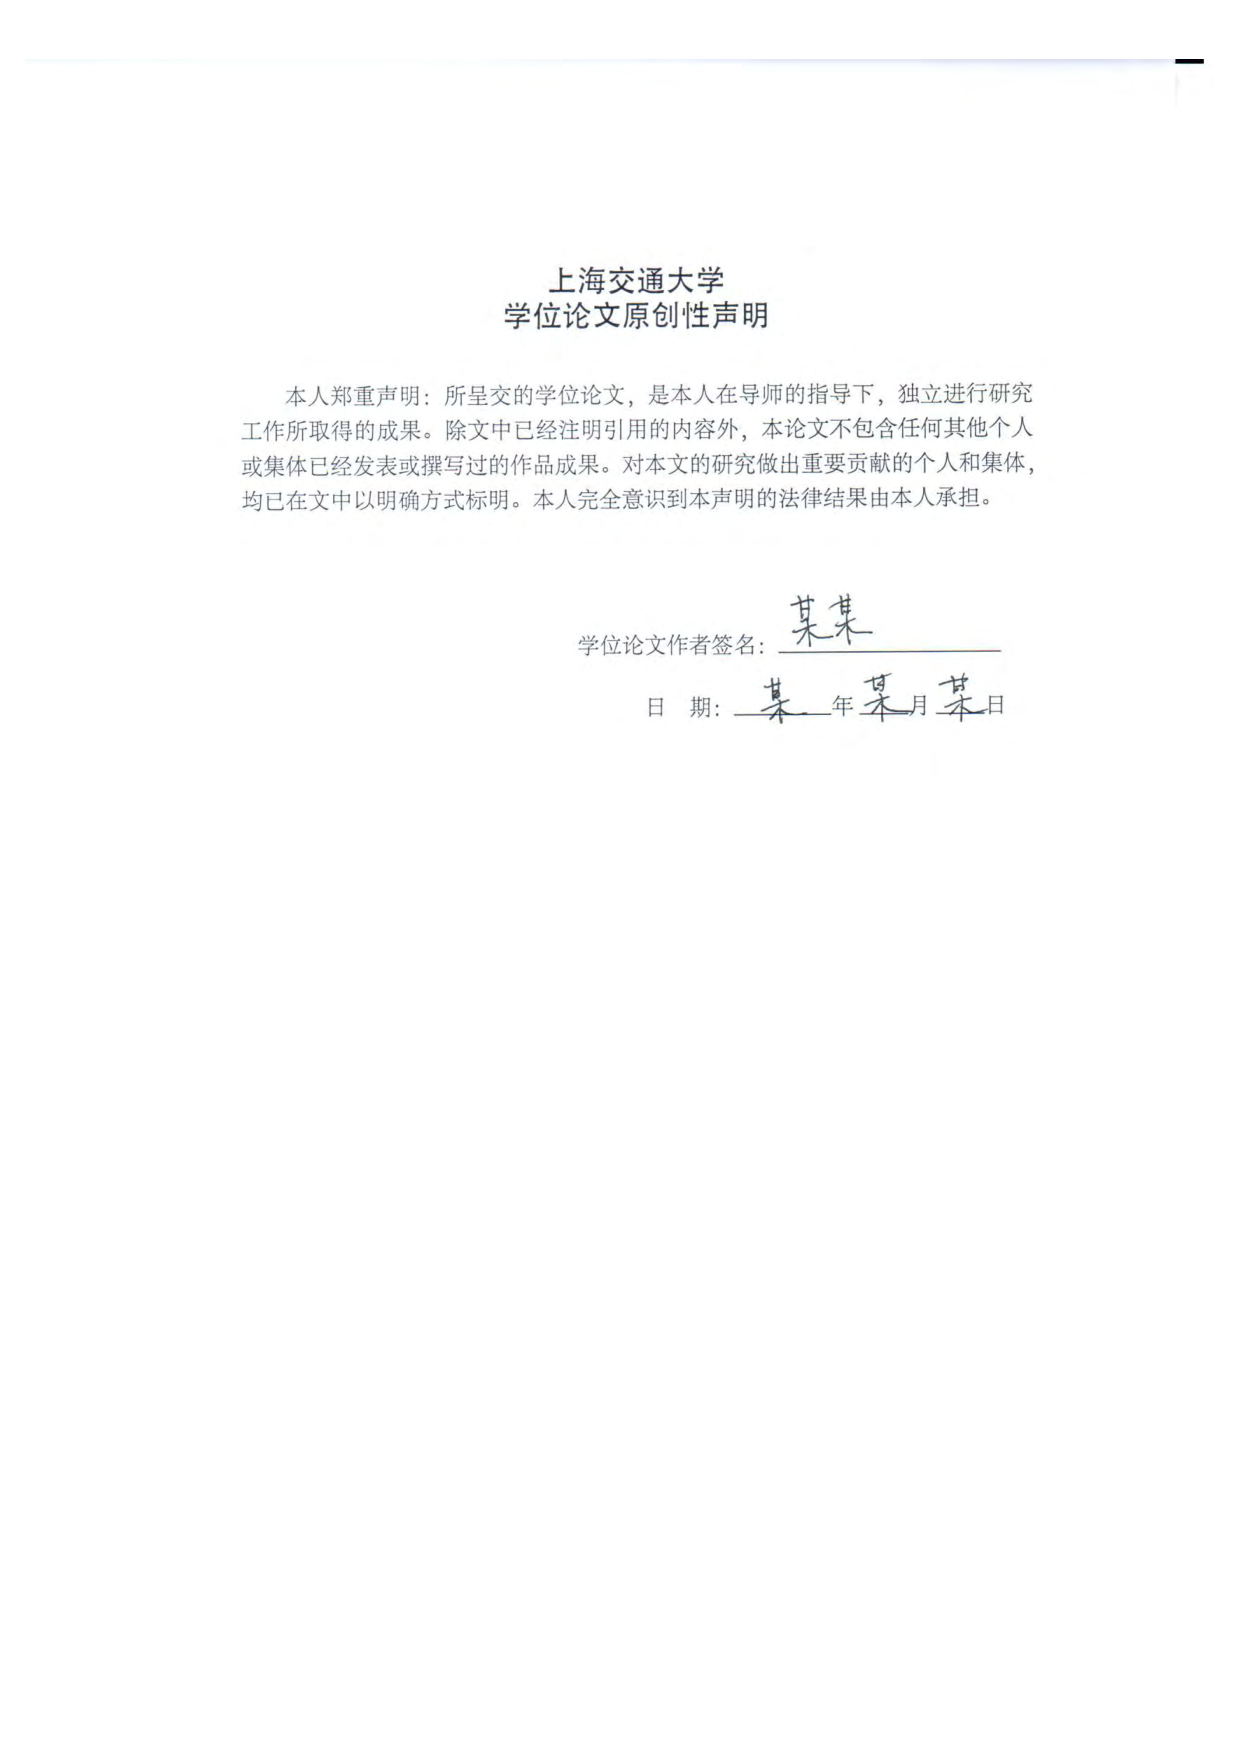
\includepdf{pdf/original.pdf}
	\cleardoublepage
	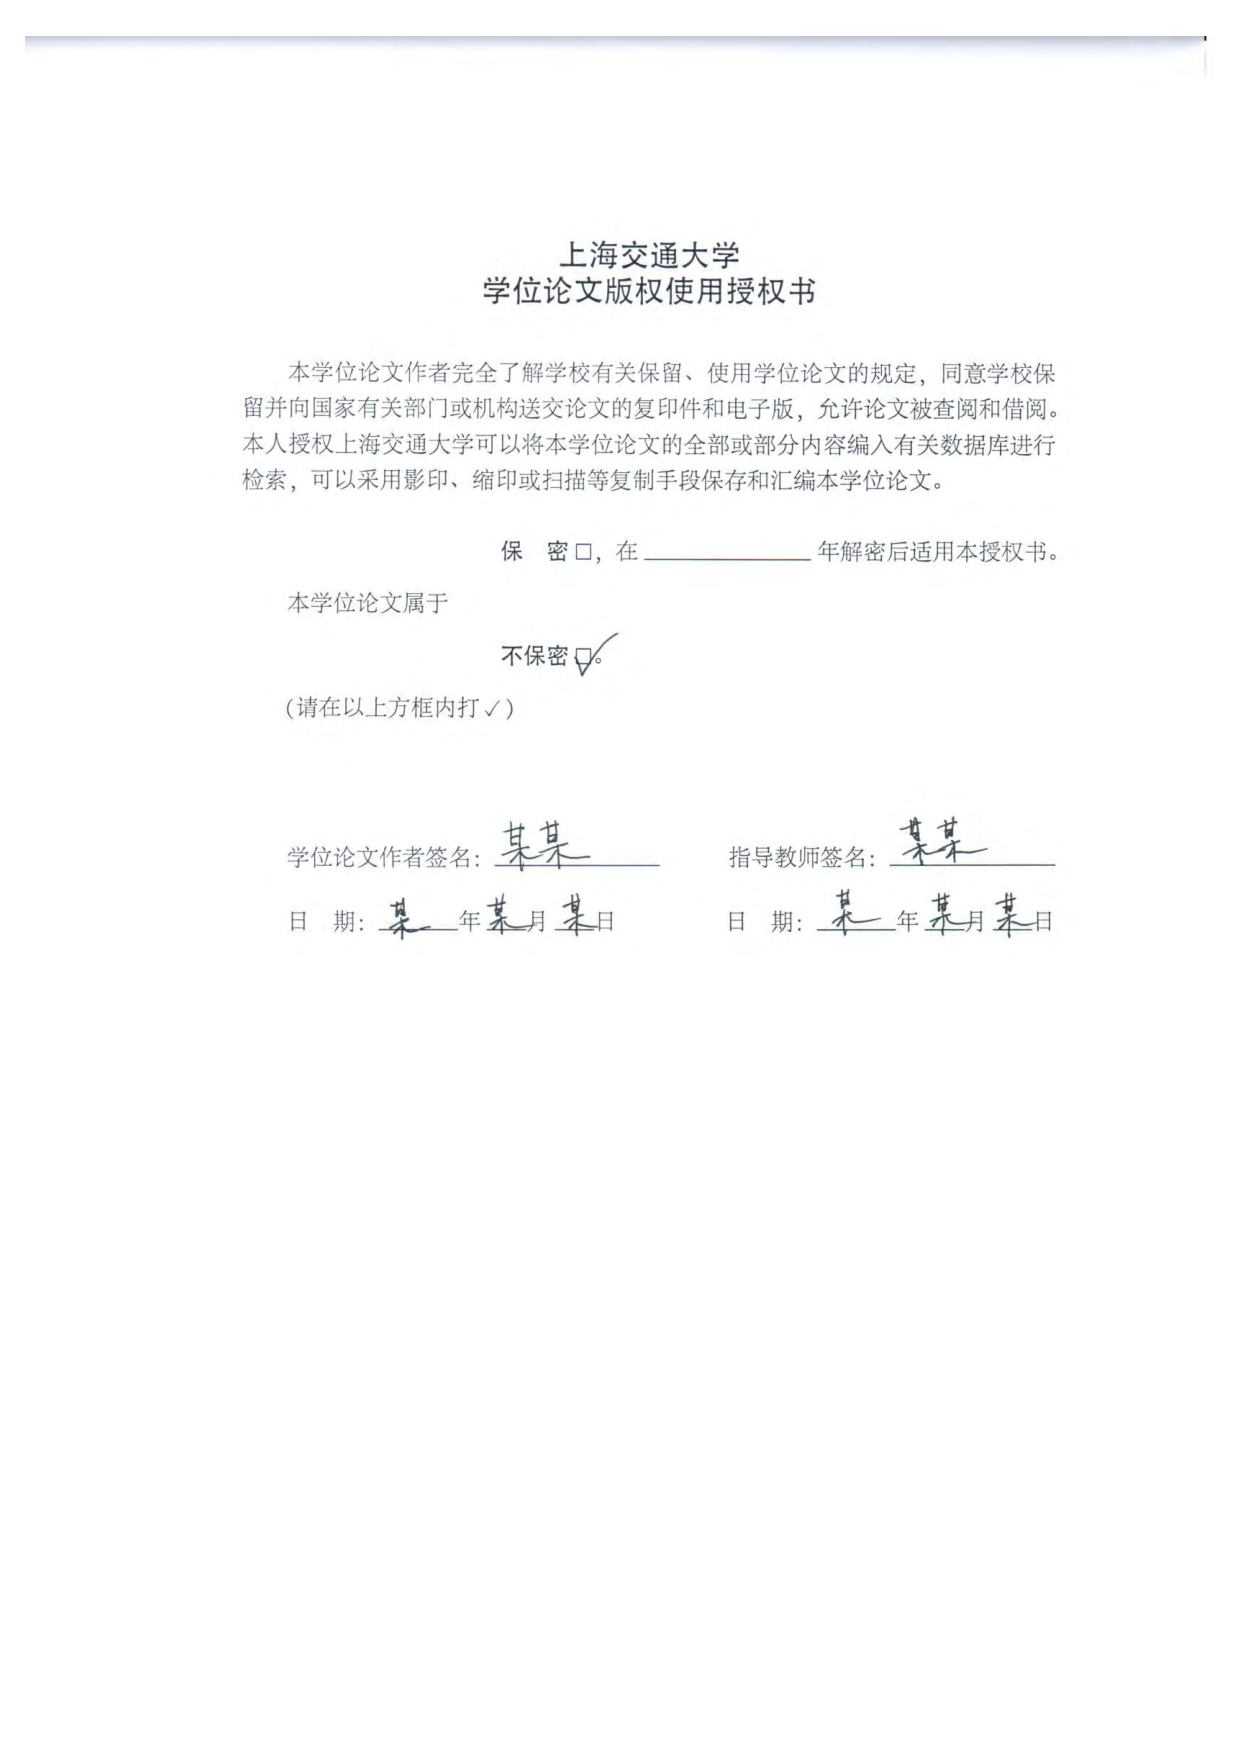
\includepdf{pdf/authorization.pdf}
	\cleardoublepage
\else
\ifsjtu@review\relax
% exclude the original claim and authorization
\else
	\makeDeclareOriginal
	\makeDeclareAuthorization
\fi
\fi
\makeatother


\frontmatter 	% 使用罗马数字对前言编号

%% 摘要
\pagestyle{main}
% !TeX root = ../thesis.tex

%# -*- coding: utf-8-unix -*-
%%==================================================
%% abstract.tex for SJTU Master Thesis
%%==================================================

\begin{abstract}
随着多种公有云和私有云架构的发展和成熟,越来越多的网络应用和计算任务被迁移至数据中心执行。数据中心建造和运行成本高昂,其中50\%以上的花费用于购买服务器硬件。然而,其服务器的平均资源利用率却通常不超过20\%。造成资源利用率低下的主要原因是大量延迟敏感型任务的存在。处理器中的计算核心共享多种计算资源,因此,并行执行的任务间存在资源竞争并将相互干扰。延迟敏感型任务受到严格的服务质量要求限制,对共享资源上的干扰十分敏感;为保证其服务质量,通常禁止其他任务与之混合执行。基于软件和硬件的资源隔离技术可以有效限制共享资源上的相互干扰,使得延迟敏感型任务与其他任务的混合执行成为可能,其有效应用的一大挑战在于多种共享资源间产生的相互干扰。本文中,我们尝试在延迟敏感型任务与其他任务混合执行的情境下,应用强化学习方法来协调多种共享资源的隔离,在保证延迟敏感型任务的服务质量的前提下,提高服务器整体的资源利用率。


\keywords{\large 数据中心 \quad 资源管理 \quad 强化学习}
\end{abstract}

\begin{englishabstract}

As public and private cloud frameworks develop and mature, an increasing number of workloads are migrating to large-scale datacenters. Typical datacenters often cost tens of million dollars, and servers are the largest fraction. However, the server utilization in most datacenters is low, often not exceeding 20\%. A primary reason for the low utilization is the popularity of latency-critical services. Each server houses several cores, and a number of resources are shared among these cores. As tasks on the same machine actively compete for shared resources, performance interferences arise. Due to strict quality-of-service(QoS) requirements, the latency-critical services are extremely sensitive to interferences. To avoid QoS violation, co-location is often disallowed for latency-critical applications in practice. Recently introduced resource isolation mechanisms allow us to mitigate these interferences.  Aiming to increase server utilization with co-location while avoiding QoS violation, we propose to build a reinforcement learning agent to automatically coordinate multiple isolation mechanisms in modern servers.

\englishkeywords{\large Data Center, Resource Management, Reenforcement Learning}
\end{englishabstract}



%% 目录、插图目录、表格目录
\tableofcontents
\listoffigures
\addcontentsline{toc}{chapter}{\listfigurename} %将插图目录加入全文目录
\listoftables
\addcontentsline{toc}{chapter}{\listtablename}  %将表格目录加入全文目录
\listofalgorithms
\addcontentsline{toc}{chapter}{\listalgorithmname} %将算法目录加入全文目录

% %# -*- coding: utf-8-unix -*-
\begin{nomenclaturename}
\label{chap:symb}

\begin{longtable}{rl}
$\epsilon$     & 介电常数 \\
 $\mu$ 		& 磁导率 \\
 $\epsilon$     & 介电常数 \\
 $\mu$ 		& 磁导率 \\
 $\epsilon$     & 介电常数 \\
 $\mu$ 		& 磁导率 \\
 $\epsilon$ 	& 介电常数 \\
 $\mu$ 		& 磁导率 \\
 $\epsilon$     & 介电常数 \\
 $\mu$ 		& 磁导率 \\
 $\epsilon$     & 介电常数 \\
 $\mu$ 		& 磁导率 \\
 $\epsilon$     & 介电常数 \\
 $\mu$ 		& 磁导率 \\
 $\epsilon$ 	& 介电常数 \\
 $\mu$ 		& 磁导率 \\
 $\epsilon$     & 介电常数 \\
 $\mu$ 		& 磁导率 \\
 $\epsilon$     & 介电常数 \\
 $\mu$ 		& 磁导率 \\
 $\epsilon$     & 介电常数 \\
 $\mu$ 		& 磁导率 \\
 $\epsilon$ 	& 介电常数 \\
 $\mu$ 		& 磁导率 \\
 $\epsilon$     & 介电常数 \\
 $\mu$ 		& 磁导率 \\
 $\epsilon$     & 介电常数 \\
 $\mu$ 		& 磁导率 \\
 $\epsilon$     & 介电常数 \\
 $\mu$ 		& 磁导率 \\
 $\epsilon$ 	& 介电常数 \\
 $\mu$ 		& 磁导率 \\
 $\epsilon$     & 介电常数 \\
 $\mu$ 		& 磁导率 \\
 $\epsilon$     & 介电常数 \\
 $\mu$ 		& 磁导率 \\
 $\epsilon$     & 介电常数 \\
 $\mu$ 		& 磁导率 \\
 $\epsilon$ 	& 介电常数 \\
 $\mu$ 		& 磁导率 \\
 $\epsilon$     & 介电常数 \\
 $\mu$ 		& 磁导率 \\
 $\epsilon$     & 介电常数 \\
 $\mu$ 		& 磁导率 \\
 $\epsilon$     & 介电常数 \\
 $\mu$ 		& 磁导率 \\
 $\epsilon$ 	& 介电常数 \\
 $\mu$ 		& 磁导率 \\
 $\epsilon$     & 介电常数 \\
 $\mu$ 		& 磁导率 \\
 $\epsilon$     & 介电常数 \\
 $\mu$ 		& 磁导率 \\
 $\epsilon$     & 介电常数 \\
 $\mu$ 		& 磁导率 \\
\end{longtable}

\end{nomenclaturename}
 % 主要符号、缩略词对照表

\mainmatter	% 使用阿拉伯数字对正文编号

%% 正文内容
\pagestyle{main}

%# -*- coding: utf-8-unix -*-
%!TEX root = ..\thesis.tex

\chapter{绪论}
随着公有云和私有云架构的发展,越来越多的的网络应用和计算任务被迁移至大规模的数据中心以减少单位计算成本,数据中心的计算能力也随之不断扩展。这些数据中心由数以万计的服务器组成,其建造和运营通常花费数千万美元以上。在现代节能型数据中心的拥有成本中,购买服务器的花费占比最高,可达50-70\%\cite{barroso2013datacenter}。一直以来,摩尔定律使得新一代服务器在相同价格下都有更高的计算能力,数据中心也得以不提高花费同时持续提升规模。然而随着暗硅(dark silicon)时代的到来\cite{esmaeilzadeh2011dark}\cite{hardavellas2011toward},这样的增长将无法持续。一种解决办法是通过使用更低能耗的组件\cite{lo2014towards},如移动计算核心\cite{janapa2010web}和移动设备中使用的内存\cite{malladi2012towards}。另一种办法是通过提高服务器的利用率---显然服务器的低利用率不但使得日常运营成本偏高,也不利于收回对设备的投资。尽管低能耗组件能够降低服务器利用率时的运营成本\cite{barroso2007case},但为了考虑到服务器的巨大资本开销,研究提高数据中心的资源利用率是最有效的,也是无法避开的。

\section{服务质量(Quality-of-Service,QoS)}
% TODO ADD MULTIPLE TIME OF REQUIREMENT LIKE SLO ETC.
数据中心不同的任务面向不同的应用和用户,因此具有不同的服务质量要求。直接面向用户的应用,如社交媒体,搜索引擎,软件即服务,在线地图,网页邮箱,在线翻译,线上购物和广告等等,通常是延迟敏感型,具有很严格的服务质量要求。延迟型敏感应用通过其内部的服务基本要求(Service Level Requirements, SLAs)定义。如谷歌搜索的服务质量通过查询的延迟和每秒处理的请求个数定义;而Bing将其定义为返回结果的质量\cite{janapa2010web}\cite{kozyrakis2010server}。

数据中心还有另一类批处理任务,如文件备份,图像离线处理和视频压缩转码等等。与延迟敏感型任务相反,他们不面向用户,延迟也不敏感,因此几乎没有服务质量要求。批量分析框架可以产生大量的批处理任务,并且这些任务即使偶尔被暂停或重启,他们仍然可以产生可观的价值\cite{boutin2014apollo}\cite{carvalho2014long}\cite{curino2014reservation}\cite{delimitrou2014quasar}。

\section{资源利用率问题}
多个研究表明,数据中心的服务器平均利用率较低,介于10\%至50\%之间\cite{kaplan2008revolutionizing}\cite{vasan2010worth}\cite{reiss2012heterogeneity}\cite{barroso2013datacenter}\cite{delimitrou2014quasar}\cite{carvalho2014long},且通常不超过20\%\cite{barroso2007case}。造成资源低利用率的主要原因是存在大量的运行在严格服务质量要求下的延迟敏感型任务。这些直接面向用户的服务的运行状态和数据通常分布在多个服务器的内存和闪存之中。各个任务的用户的访问模式存在差异,因而每个任务的负载相差较大。然而,由于延迟敏感型任务普遍巨大的数据量和高昂的移动代价,这些服务难以被集中在少量服务器中,因而难以优化他们的计算资源利用率。

数据中心的服务器通常区有2-4个处理器插口,每个插口上有4-10个核心。核心之间共享一些资源,如末级高速缓存(Last Level Cache,LLC),动态随机存储器,输入输出通道,网络连接。这种共享使得各个核心之间产生难以预测的干扰,而即使轻微干扰便可能导致延迟敏感型任务违反服务质量要求\cite{janapa2010web}\cite{nesbit2006fair}\cite{meisner2011power}。为了避免违反服务质量要求,通常禁止在运行延迟敏感任务的服务器上执行其他任务。这样过度的限制使得延迟敏感型任务独占服务器,部分核心空闲,系统的资源利用率降低。例如,Google用以运行网页搜索服务的服务器24小时内的平均空闲率为30\%\cite{lo2014towards}。对延迟敏感型任务的过度保护代价高昂,同时也是不必要的。制定合理的混合执行策略可以有效提高服务器资源利用率\cite{delimitrou2013paragon}\cite{mars2011bubble}\cite{marshall2011improving}。

\section{混合执行}
数据中心的应用通常由一至数百个任务组成,每个任务有其单独的二进制程序,相关数据,以及一个声明其所需求资源的配置文件\cite{mishra2010towards}。配置文件一般包括其需要的核心数量,内存大小,硬盘空间和是否需要禁止与其他任务混合执行。一个任务调度的简化版本可见\ref{fig:schedule}。集群级别的任务调度器收到任务时,通过类似装箱问题的算法将各个任务分配至集群内的服务器上运行\cite{mishra2010towards}。当任务到达指定服务器上时,服务器级别的资源调度器将会控制任务的执行\cite{banga1999resource}。任务的资源需求通常由管理员精心配置以满足其服务质量要求。禁用混合执行的延迟敏感型任务不可避免的会占用更多的服务器资源,进而导致资源利用率下降。延迟敏感型任务严格的服务质量要求,使得我们似乎必须在延迟敏感型任务的服务质量和资源利用率之间做出选择。事实是,延迟敏感型任务独占服务器的策略通常是不必要的--尽管其他任务的执行会降低延迟敏感型任务的服务性能,但并非一定导致其违反服务质量要求。图\ref{fig:colocate}(a)表示一个来自谷歌搜索的关键组件的性能(以响应延迟的倒数表示)随同一处理器上混合执行的其他任务的影响的变化,可以看出当来自混合执行任务的干扰较低时,延迟敏感型任务的性能依然可满足服务质量要求\cite{mars2011bubble}。图\ref{fig:colocate}(b)显示了该搜索组件与多种具体任务混合执行时产生的性能下降,可以看到该搜索组件与地图等任务混合执行时仍能达到规定的服务质量;而其与广告等任务混合执行时,将产生显著的性能下降,且违反服务质量要求。

\begin{figure}
  \centering
  \begin{subfigure}{0.4\textwidth}
    \centering
    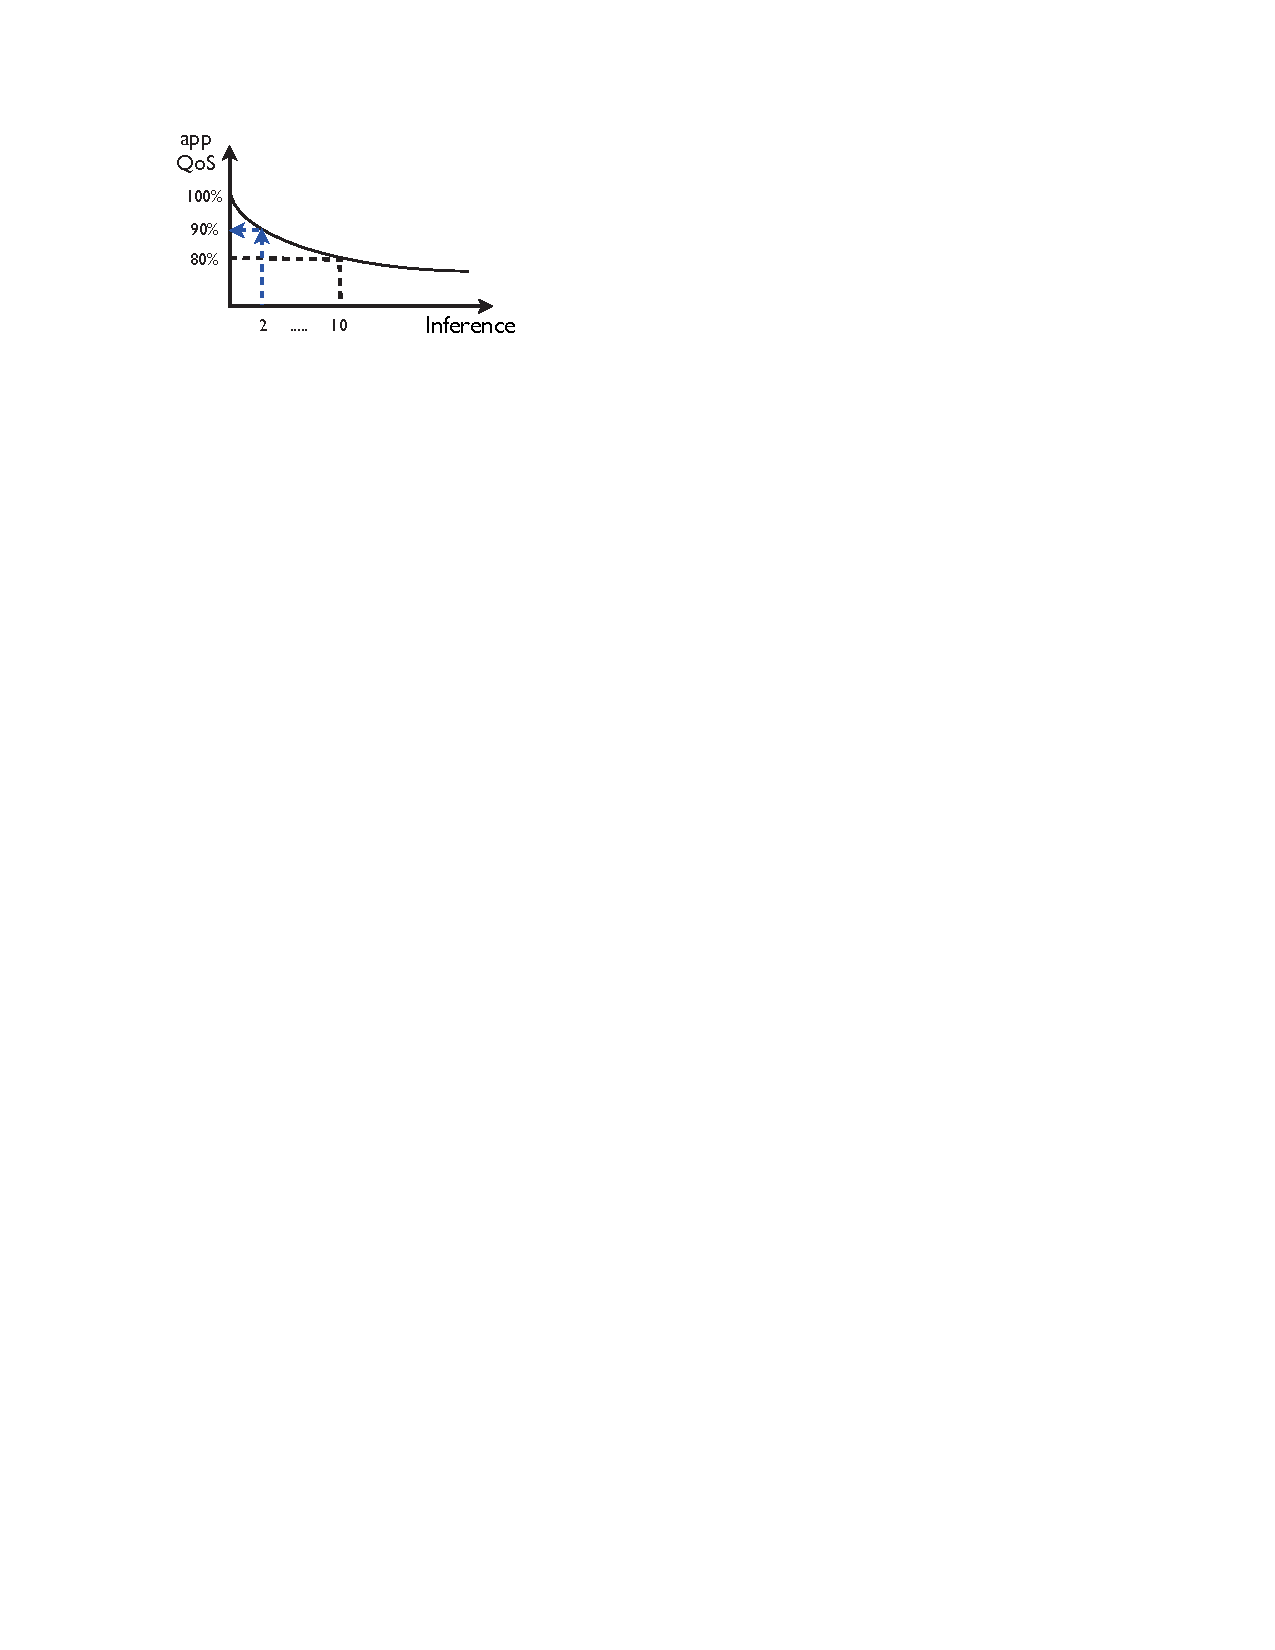
\includegraphics[height=4cm]{res_mgmt/qos_pressure.pdf}
    \caption{延迟敏感型任务服务质量随干扰强度的变化}
  \end{subfigure}
  \hspace{1em}
  \begin{subfigure}{0.55\textwidth}
    \centering
    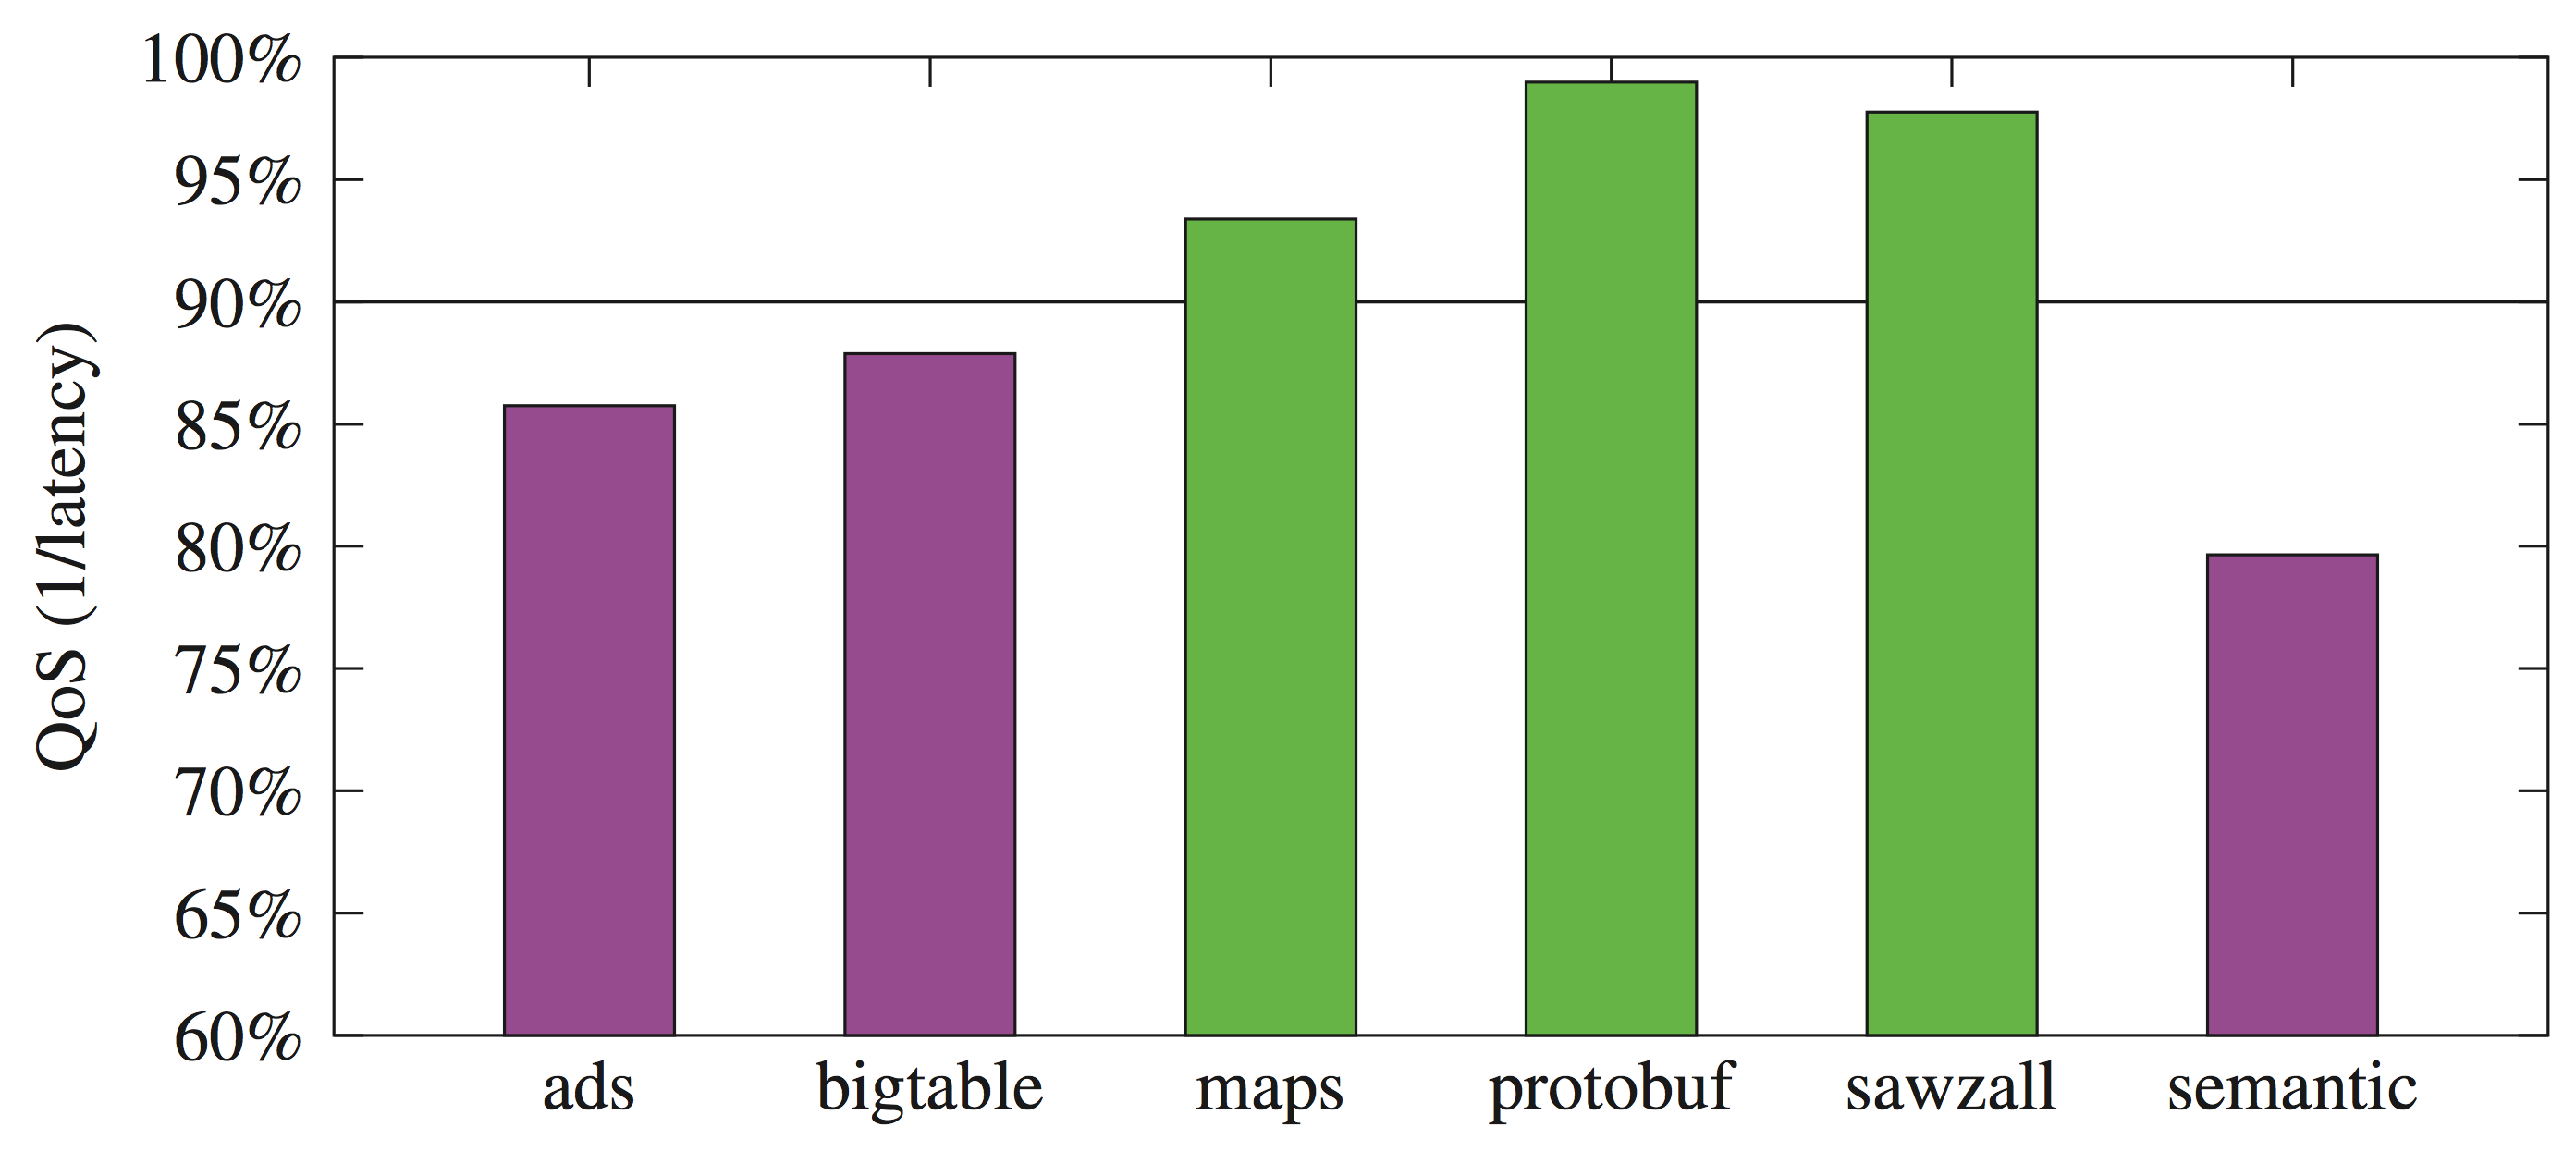
\includegraphics[height=4cm]{res_mgmt/colocate.png}
    \caption{搜索任务在混合执行时的服务质量下架}
  \end{subfigure}
  \captionof{figure}{混合执行与服务质量下降}
  \label{fig:colocate}
\end{figure}

合理地混合执行延迟敏感型任务与批处理任务,使批处理任务有机会利用延迟敏感型任务没有足够利用的资源,有利于提高整体资源利用率。混合执行的一个主要挑战在于难以确定批处理任务对共享资源产生影响,其对延迟敏感型任务的干扰更是难以预测。正因为如此,关于混合执行的研究通常关注吞吐量的任务和批处理任务的混合\cite{cook2013hardware}\cite{nathuji2010q}。

\begin{figure}
  \centering
  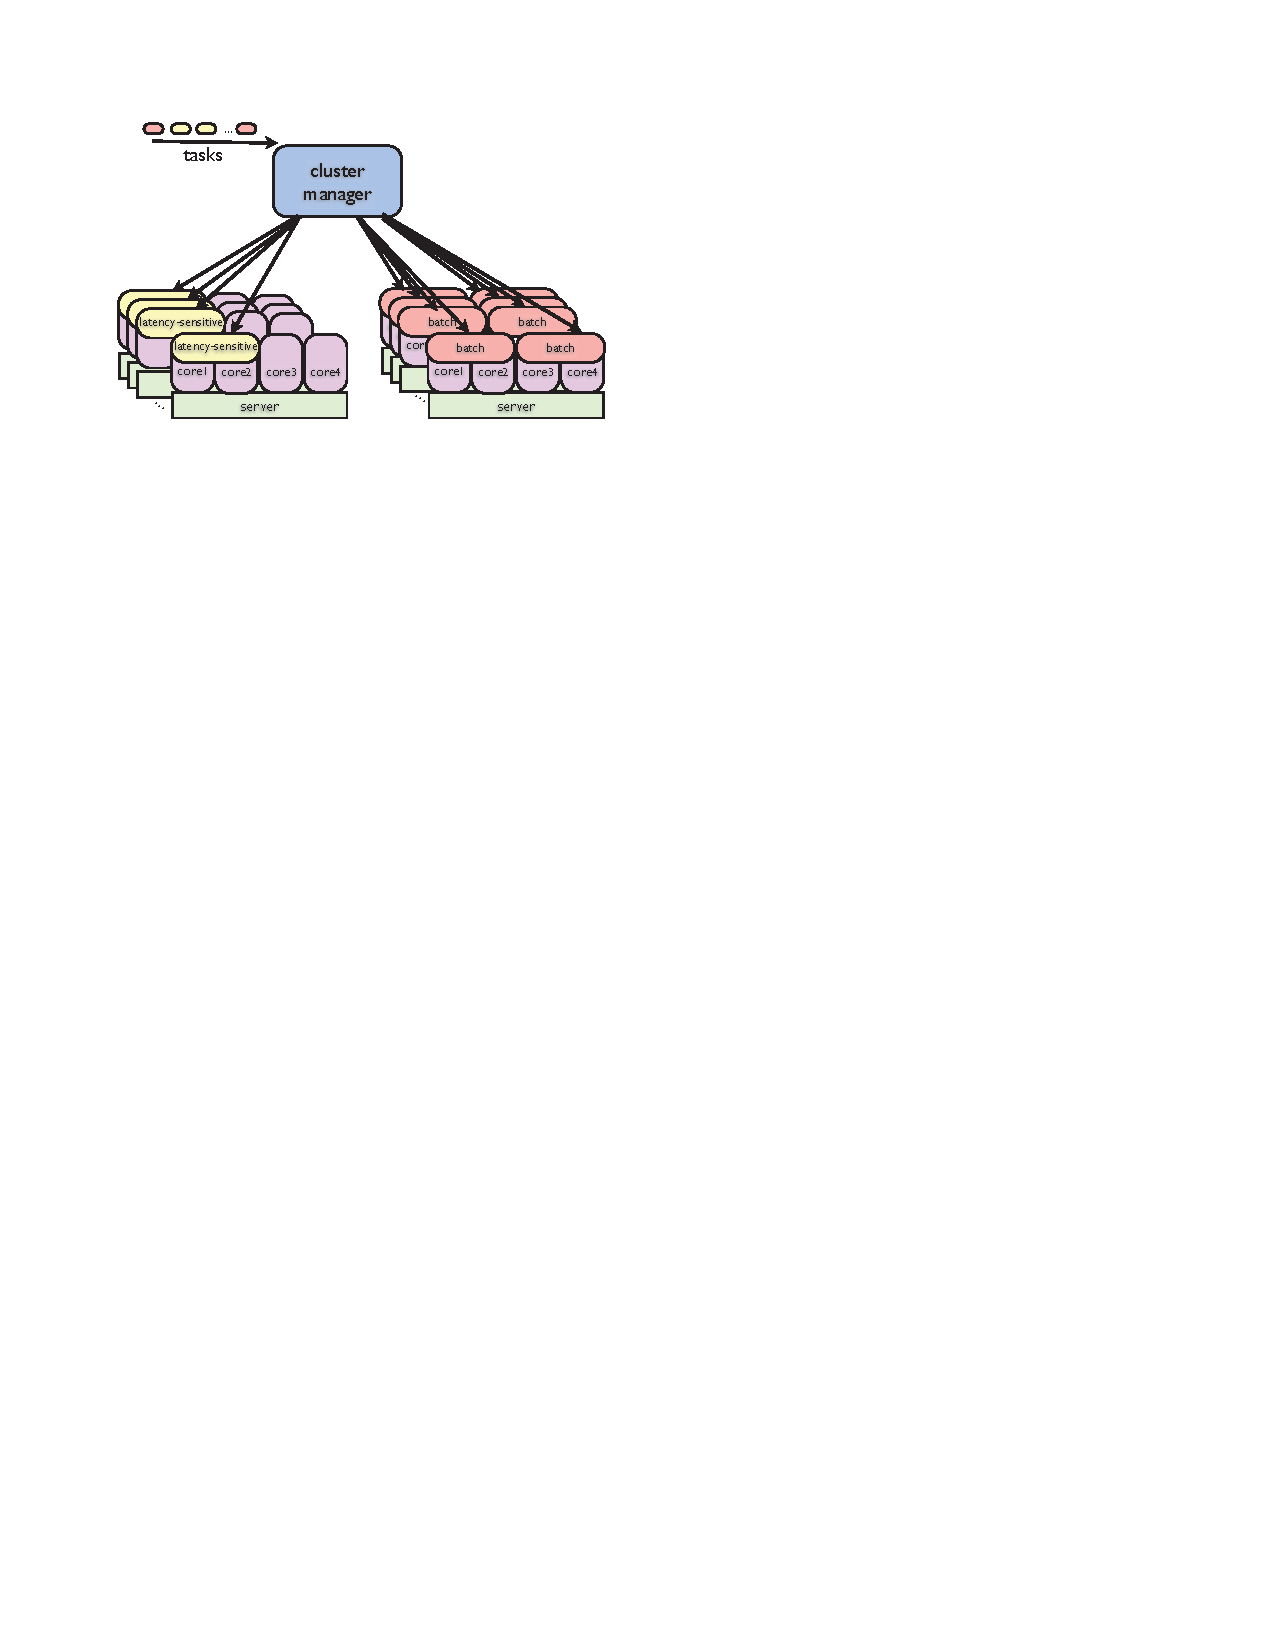
\includegraphics[width=0.65\linewidth]{res_mgmt/schedule.pdf}
  \captionof{figure}{数据中心集群级任务调度}
  \label{fig:schedule}
\end{figure}

\section{气泡测试(Bubble-Up)}
确定延迟敏感型任务和批处理任务的混合执行策略是困难的。批处理任务对延迟敏感型任务产生的性能影响很难准确预测,这导致了大部分延迟敏感型应用直接禁止混合执行。若无法对其影响准确预测,指定混合执行策略的唯一途径则只能是一一测试不同的任务混合执行的效果。对$\mathrm{N}$个任务进行测试,则需要$\mathrm{O(N^2)}$次实验。对于数据中心成百上千的应用程序和其频繁的升级更新,这种蛮力测试的代价显然是无法接受的。

Mars等人提出了气泡测试的方法来预测混合执行任务之间相互的性能影响\cite{mars2012increasing}。气泡测试将预测混合执行的任务之间的相互干扰分为两部分,一部分是任务受共享内存系统压力导致的性能下降,另一部分为其本身对共享内存系统造成的压力,如图\ref{fig:bubble}所示\cite{mars2012increasing}。第一步,通过精心设计的气泡(测试任务)来测试目标任务对内存子系统压力的的敏感程度;第二步通过测试目标任务对气泡造成的影响来预测其系统造成的压力。当混合执行导致的性能下降可以低廉代价准确预测时,即可通过类似装箱的算法找到充分利用服务器资源而不至于使延迟敏感型任务违反服务质量代价的混合策略。


气泡测试可以准确的预测延迟敏感型任务在不同程度资源竞争条件的性能下降,并以此生成任务混合策略。任务的混合执行使得服务器的资源利用率提高,然而在生成混合策略时必须考虑到延迟敏感型任务最大的资源需求。延迟敏感型任务通常面向用户,其负载虽具有固定的访问模式,但具有无法预测的访问高峰。这样的差异意味着延迟敏感型任务在相当时间内并没有全部利用预留的资源。任何静态的混合执行策略要么过于保守——导致资源利用率不足;要么过于乐观——导致延迟敏感型任务违反其服务质量要求\cite{lo2015heracles}。

解决此问题的一个办法是使用动态的混合执行策略,在应用程序高峰与低谷时执行不同的混合策略。当延迟敏感型任务处于低负载时,将其与较多占用共享资源的批处理任务混合执行;当延迟敏感型任务的负载上升时,将高共享资源占用的批处理任务迁移至其他服务器,并调度较低共享资源占用的批处理任务至当前服务器。延迟敏感型任务负载的高峰通常难以预测,且数据中心任务较大的运行时数据意味着高昂服务器间迁移任务的代价。同时,迁移任务所需的计算能力、缓存占用、网络带宽使用也会对资源敏感型任务的服务质量造成压力。另外,动态混合策略还可能存在已进行计算的进度难以保存的问题。因此通过动态的混合执行策略来提高服务器资源利用率并不实际。

另一个解决静态混合执行策略的办法则是按延迟敏感型处在低强度负载时的性能需求来确定能与之并行执行的批处理任务。这样的批处理任务具有更高的资源需求,可以在延迟敏感型任务低负载时充分利用服务器资源;在延迟敏感型任务高强度负载时并需要的大量的服务器资源时,通过资源隔离的机制保证其性能。
\begin{figure}[!t]
  \centering
    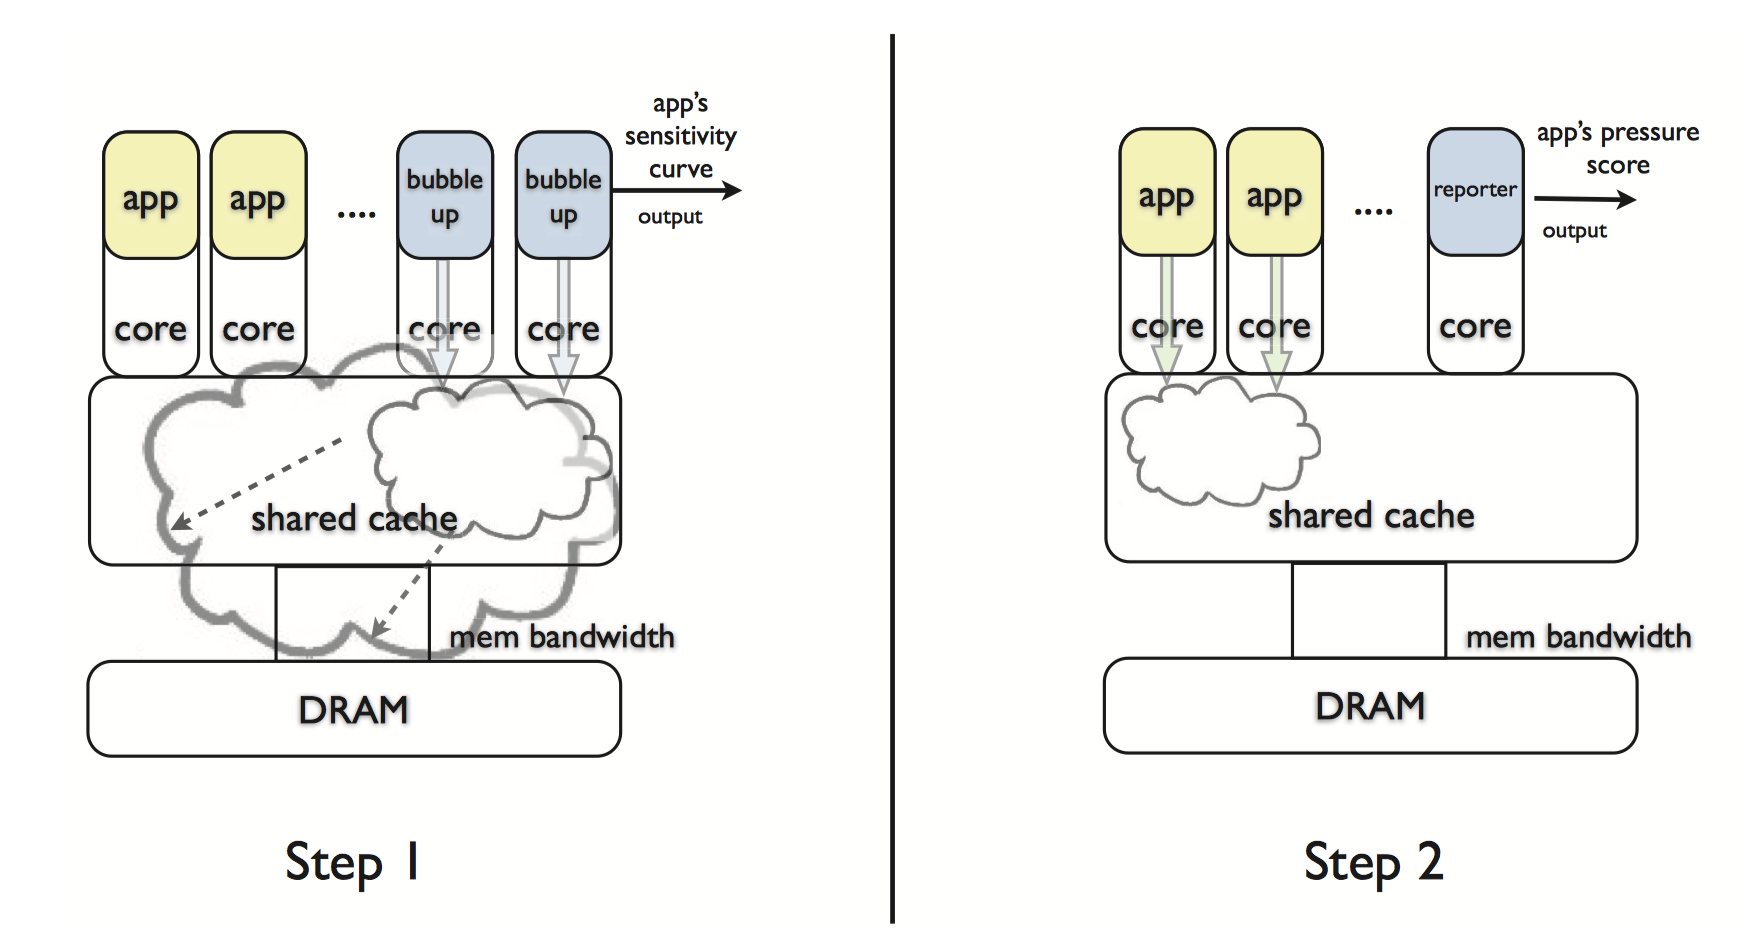
\includegraphics[width=0.95\linewidth]{res_mgmt/bubble.png}
    \captionof{figure}{气泡测试方法}
    \label{fig:bubble}    
\end{figure}
\section{资源隔离技术}
敏感型任务与批处理任务混合执行时,共享资源的相互干扰使得我们难以控制批处理任务对延迟敏感型任务的影响,进而难以保证不违反延迟敏感型任务的服务质量要求。一个典型的混合执行的任务之间在共享资源上相互干扰的例子是吵闹的邻居问题\cite{verboven2013black},即混合执行的任务在某一个或多个共享资源上进行了过多的占用。图\ref{fig:neigbor}中,蓝色线表示延迟敏感型任务的性能,红线表示批处理任务的性能。可以看到,当批处理任务不受限制地占用共享资源时,延迟敏感型任务的性能将因此出现显著下降。批处理任务不公平和不受控制的占用共享资源可能来自多个方面。

\begin{itemize}
  \item 批处理任务具有很高的并行性,因此产生了大量的进程或线程并行执行并由此抢占大量的处理器运行时间;
  \item 批处理任务使用大规模数据集且频繁读写,由此占用大部分的共享缓存和动态随机存储访问带宽,使得批处理任务的缓存命中率降低和动态随机存储器的访问延迟上升;
  \item 延迟敏感型任务使用的TCP协议在检测到网络阻塞时会主动降低带宽占用,当批处理任务使用UDP等没有流量控制的协议,批处理任务的流量不受限制的挤压延迟敏感型任务的网络带宽。
\end{itemize}

\begin{figure}
  \centering
    \centering
    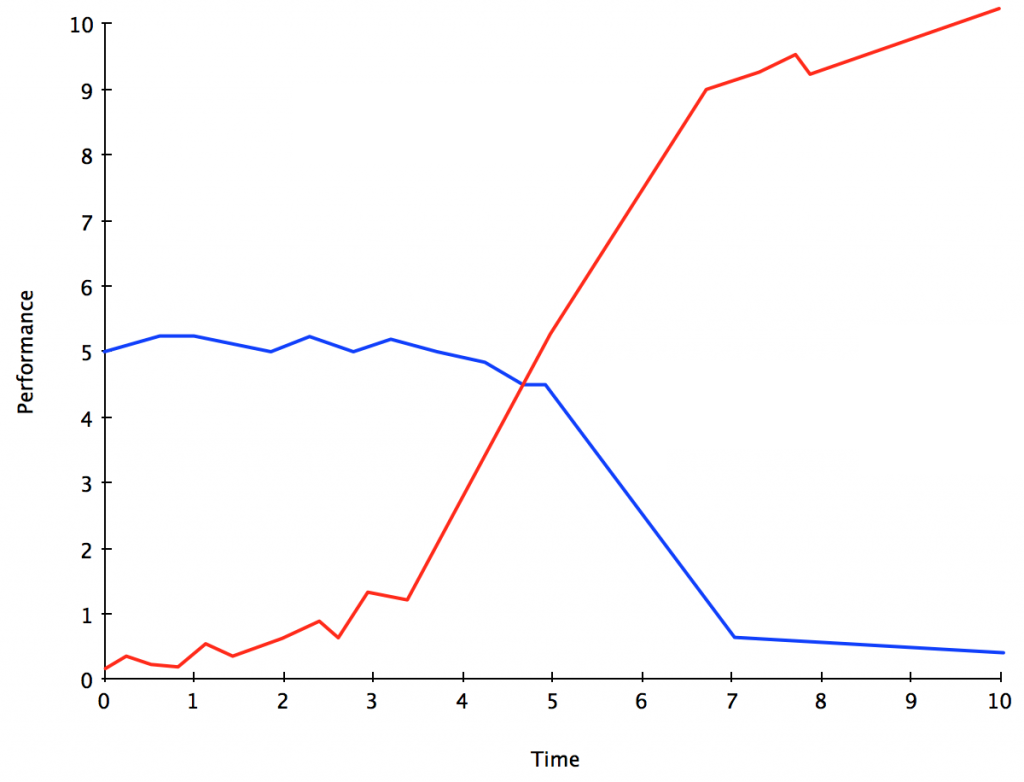
\includegraphics[width=0.6\linewidth]{res_mgmt/neighbor.png}
    \captionof{figure}{吵闹的邻居}
    \label{fig:neigbor}  
\end{figure}


混合执行任务在共享资源上相互干扰的问题,使得延迟敏感型任务的性能下降和出现不稳定,保证其服务质量成为难题。新出现的一些资源隔离技术可以让我们在单个服务器中动态分配共享资源,使得我们能够通过同时协调多种资源的分配,在采用更激进的混合执行策略的同时,改善混合执行对延迟敏感型任务服务质量的影响。

\subsection{计算核心}
核心的共享对延迟敏感型任务的服务质量影响巨大\cite{lo2015heracles},英特尔处理器的超线程技术使得问题更加复杂化。我们通常不允许延迟敏感型任务和批处理任务共享一个逻辑核心(一个超线程),因为在共享逻辑核心时,操作系统内核的调度会增加即使毫秒的延迟\cite{leverich2014reconciling}。另外当同属一个物理核心的两个超线程同时执行延迟敏感型任务和批处理任务,他们将共享指令带宽,一/二级高速缓存和页表缓存。实验表明,当延迟敏感型任务与其他计算密集或访存密集的任务共享同一物理核心时(运行在不同逻辑内核上),敏感型任务的服务质量会出现显著下降\cite{lo2015heracles}。

通过Linux的\textit{cgroup}框架\cite{menage2008cgroups}我们可以将延迟敏感型任务和批处理任务隔离在不同的逻辑核心子集上。随着服务器的逻辑计算核心数目增多,这样的资源调度也更为细粒度。计算核心的分配可以动态调节,调节的速度取决于Linux内核可以在多快时间内将任务从一个核心迁移到另外一个核心,这通常在几十毫秒左右。

\subsection{末级高速缓存}
同一处理器接口上的核心共享末级高速缓存。多个研究表明共享末级高速缓存中不受控制的干扰会严重影响混合执行任务的性能\cite{delimitrou2014quasar}\cite{govindan2011cuanta}\cite{leverich2014reconciling}\cite{mars2012increasing}\cite{sanchez2011vantage}。混合执行任务在末级高速缓存上不受控制的干扰是一个典型的吵闹的邻居问题,如图\ref{fig:cache_diagram}。图\ref{fig:cache_diagram}(a)中,批处理任务有高频率的数据读取需求,在没有末级高速缓存隔离时,批处理任务占用了大量的缓存容量。对延迟敏感型任务来说,尽管通过计算核心隔离技术获得了较大的计算核心资源,其实际可用的缓存大小却严重低于需求,引起缓存命中率的将下降,整体性能也将下降。当延迟敏感型任务处于高负载状态时,轻微的相互干扰会引起巨大的延迟\cite{kasture2014ubik},因此末级高速缓存的干扰可能造成延迟敏感型任务违反服务质量要求。

\begin{figure}
  \centering
  \begin{subfigure}{0.4\textwidth}
    \centering
    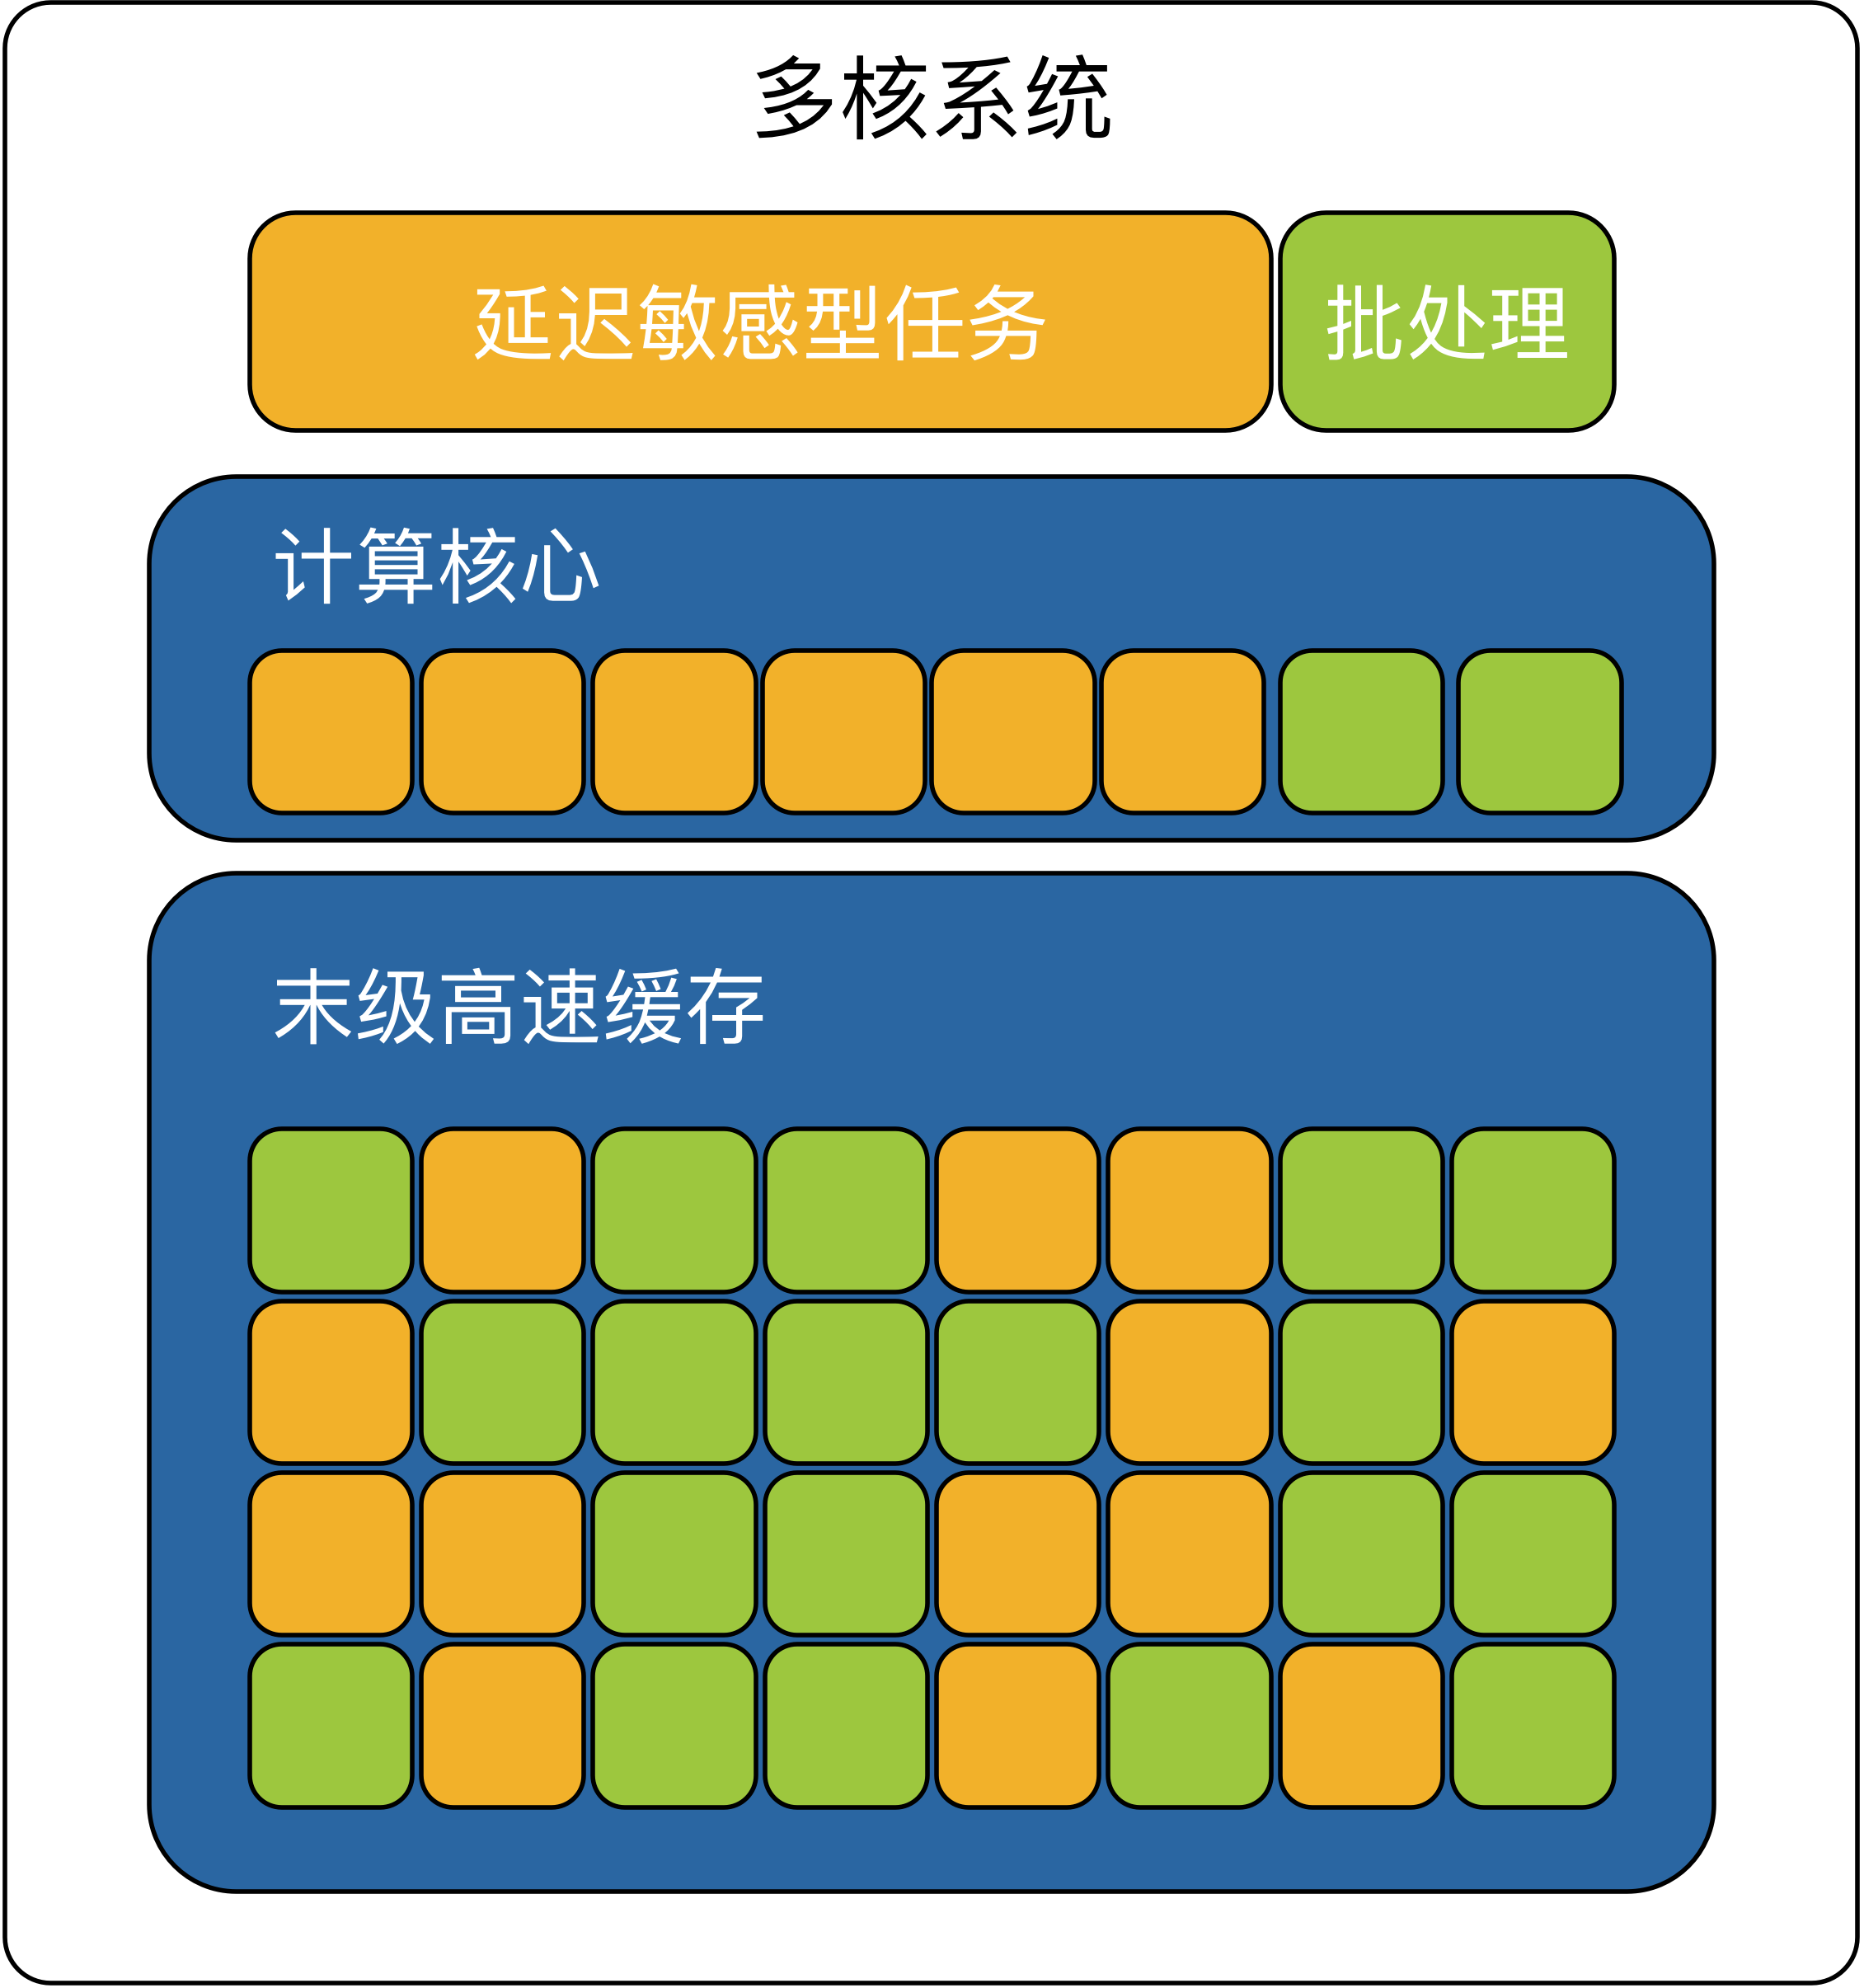
\includegraphics[height=7cm]{res_mgmt/cache_diagram_a.png}
    \caption{批处理任务过多占用缓存}
  \end{subfigure}
  \hspace{3em}
  \begin{subfigure}{0.4\textwidth}
    \centering
    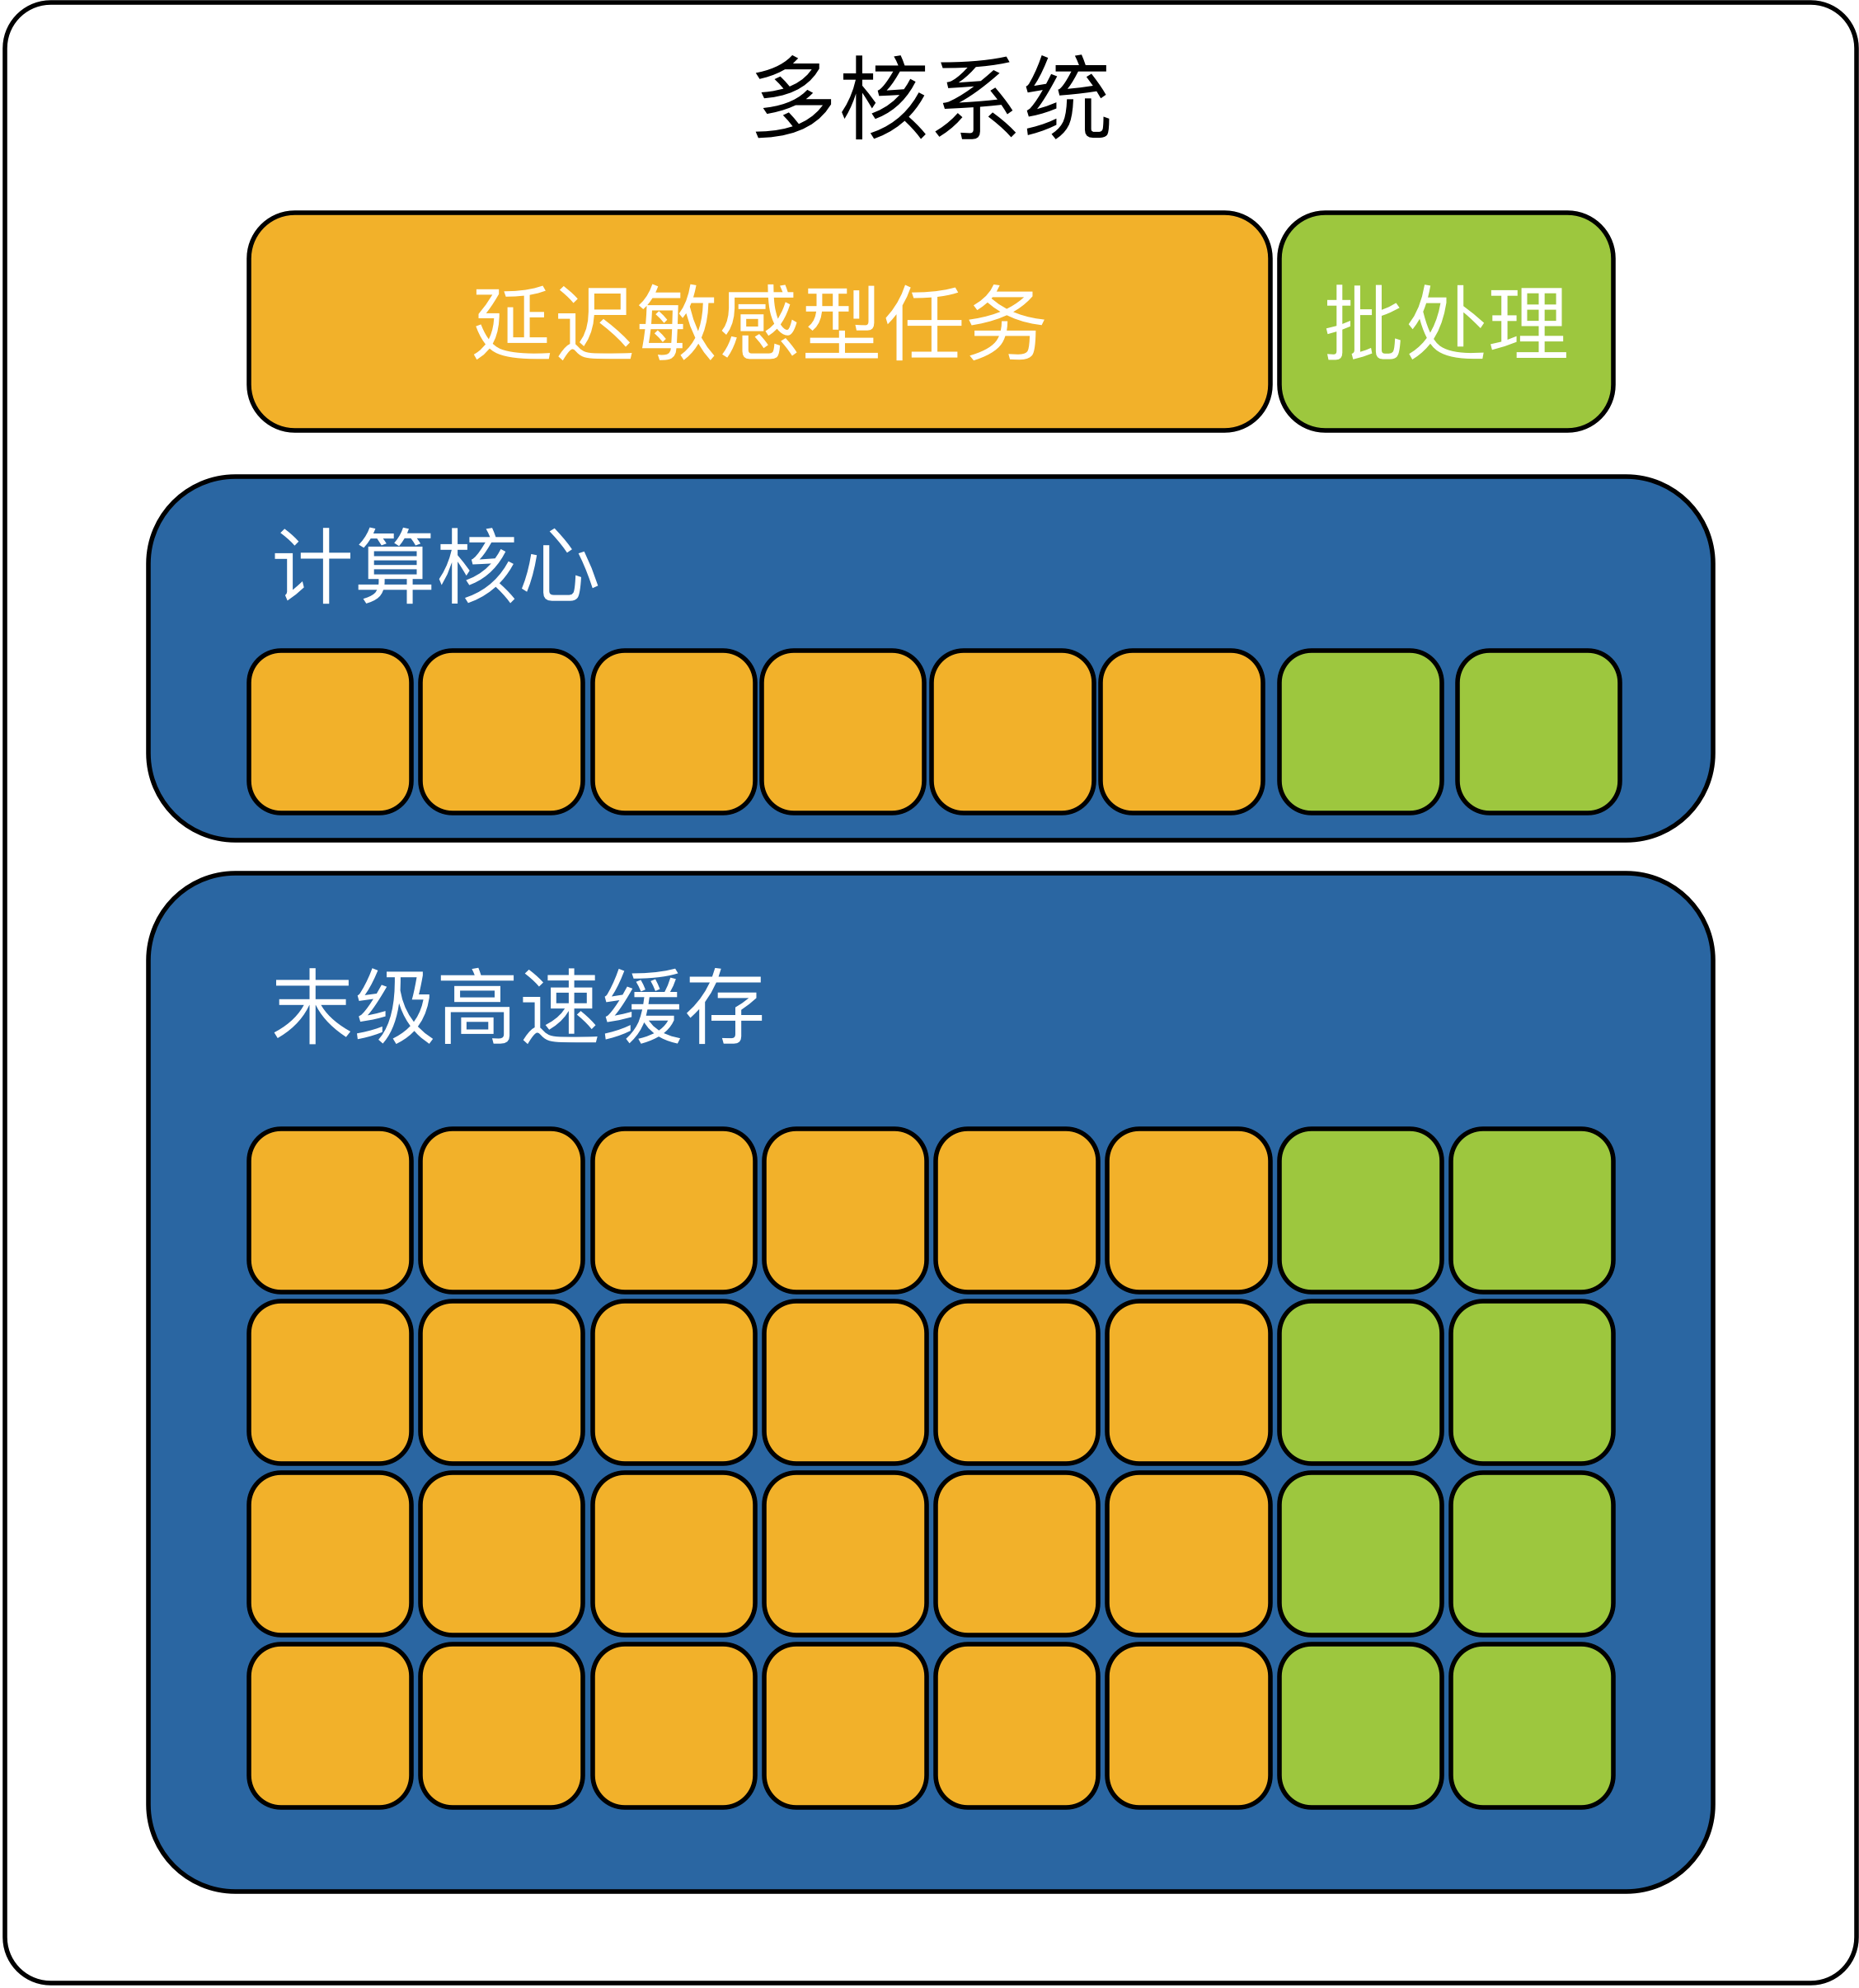
\includegraphics[height=7cm]{res_mgmt/cache_diagram_b.png}
    \caption{缓存分配技术隔离缓存使用}
  \end{subfigure}
  \captionof{figure}{末级高速缓存上的相互干扰}
  \label{fig:cache_diagram}
\end{figure}


% Thread ID and cache line
混合执行任务抢占末级高速缓存的问题一直无法有效解决,直到近期硬件支持的资源管理技术的出现。英特尔自Xeon E3引入的缓存分配技术(Cache Allocation Technology, CAT)基于硬件实现了末级高速缓存按路分配管理\cite{guide2011intel}。缓存分配技术将末级缓存按组关联路数划分成更小的缓存子集。当核心被分配给某一缓存子集后,可以在缓存任何位置命中,但新读取的数据只能写入其被分配的子集之中。通过缓存分配我们可以为延迟敏感型任务和批处理任务分配不相重叠的末级高速缓存以限制批处理任务在末级缓存处对延迟敏感型任务产生的压力。即使是将批处理任务与只关注吞吐量的任务混合执行时,通过硬件或软件技术动态分配末级高速缓存也是被普遍偏好的做法\cite{cook2013hardware}\cite{iyer2007qos}\cite{qureshi2006utility}\cite{lin2008gaining}\cite{nathuji2010q}。改变缓存分配可以通过写特定寄存器(Model Specific Register, MSR)动态实现并在在数毫秒内生效,其粒度通常在末级高速缓存大小的5\%左右\cite{herdrich2016cache}。Linux内核自4.10起通过虚拟文件系统resctl也实现了对缓存分配技术的支持。

通过缓存分配技术,我们可以实现混合执行任务间末级高速缓存资源的隔离。图\ref{fig:cache_diagram}(b)中,通过缓存分配技术,延迟敏感型任务被分配与之计算核心资源成比例的末级高速缓存容量,避免了来自批处理任务的干扰以获得稳定的服务性能。图\ref{fig:cat_perf}显示压缩任务Bzip2与各种任务混合执行时,缓存分配技术(CAT)的使用对其性能的稳定作用\cite{herdrich2016cache}。可以看到Bzip2对来自部分产生较大缓存压力的应用的干扰敏感;同时还能看到,合理的隔离不同任务对末级高速缓存的共享(实验中为Bzip2分配50\%的末级高速缓存),使得Bzip2任务在混合执行条件下基本保持与单独执行时一致的性能。

\begin{figure}
  \centering
  % \begin{minipage}[b]{0.6\textwidth}
    \centering
    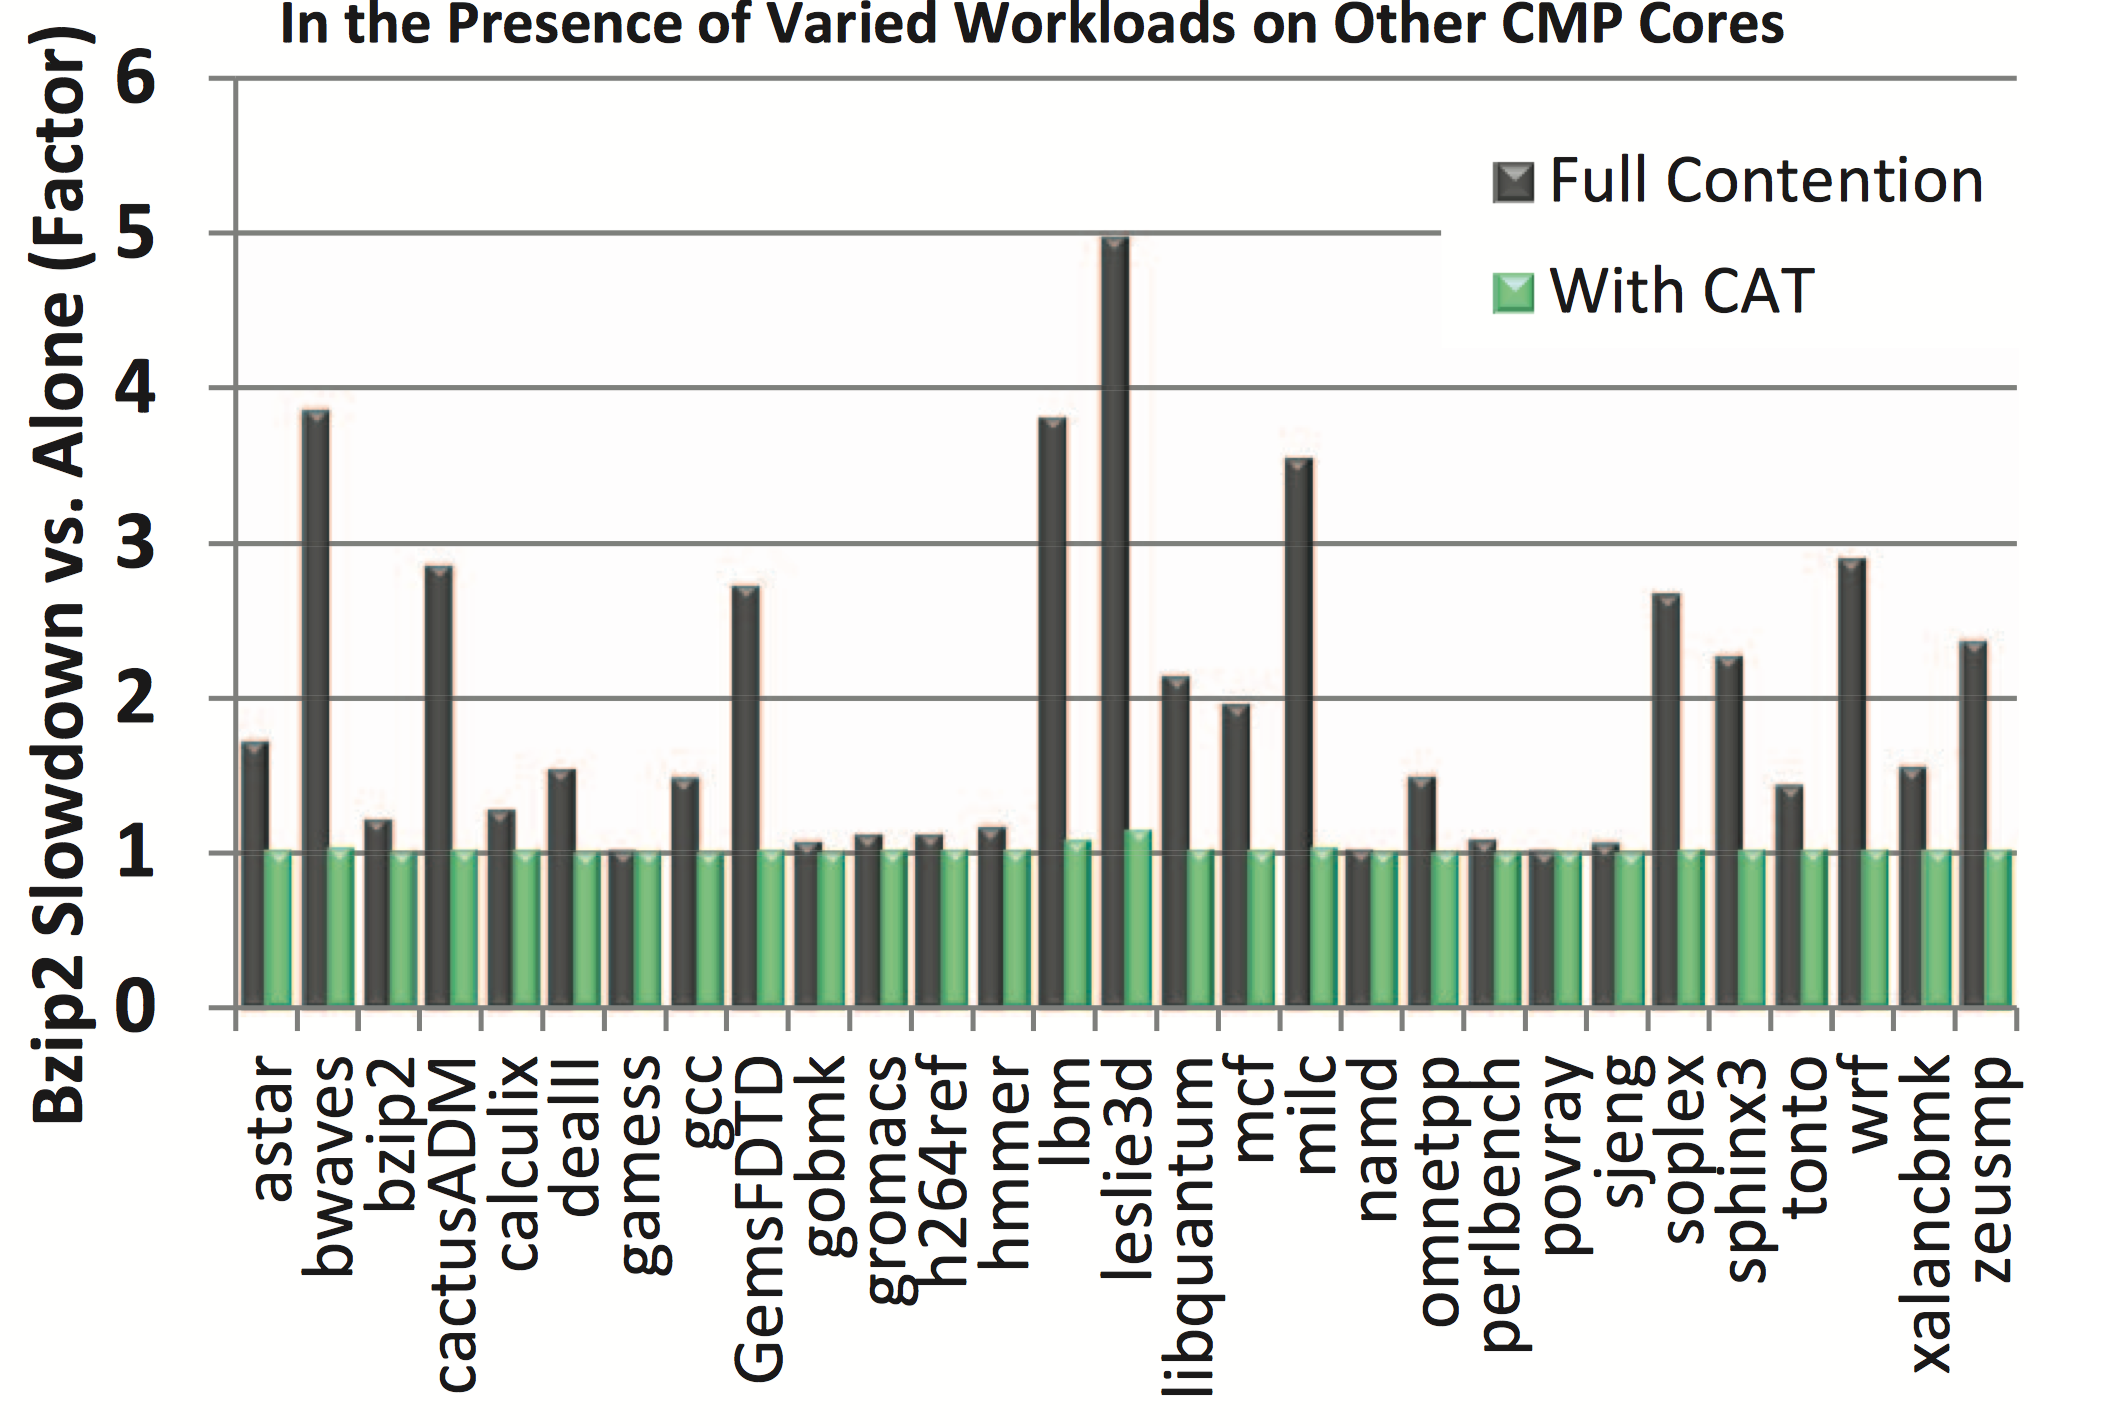
\includegraphics[width=1\linewidth]{rl/cat_perf.png}
    \captionof{figure}{Bzip2混合执行时的性能下降}
    \label{fig:cat_perf}
  % \end{minipage}     
\end{figure}

\subsection{动态随机存储器访问带宽}
数据中心的大部分的任务,无论是延迟敏感任务或批处理任务,都运行在较大的数据集之上,无法载入片上高速缓存。因此,这些任务在执行时都将占用动态随机存储器的访问带宽,且对混合执行的任务访问动态随机存储产生干扰。当批处理任务的末级高速缓存使用受限后,其末级缓存的命中率也会降低,导致其对动态随机存储的访问增加并占用更多的访存带宽。批处理任务占用更高的动态随机存储器访问带宽意味着当延迟敏感型应用内存读写的代价升高,进而可能导致其违反服务质量要求。因此动态控制批处理任务的动态随机存储器带宽占用有利于减小资源敏感型任务读写内存性能受到的干扰。

已有大量的研究致力于解决混合执行任务的动态随机存储访问上的相互干扰\cite{iyer2007qos}\cite{jeong2012qos}\cite{muralidhara2011reducing}\cite{nesbit2006fair}。最新的英特尔处理器引入了内存带宽分配(Memory Bandwidth Allocation, MBA)技术和内存带宽监控(Memory Bandwidth Monitoring)技术\cite{iyer2007qos}\cite{guide2011intel}。内存分配技术仅在部分新处理器可用,大部分处理器硬件仅支持内存带宽监控\cite{guide2011intel}。幸运的是,基于硬件且粒度为单个核心的内存带宽监控配合动态的计算核心分配技术,我们能够粗粒度的调控批处理任务对动态随机存储器访问带宽\cite{lo2015heracles}。当监测到批处理任务过多占用内存访问带宽而延迟敏感型任务受限与此时,可以通过减少为其分配的计算核心以降低其带宽占用。尽管如此,缺少硬件支持的对动态随机存取器访问带宽的直接调控限制了在混合执行时保证延迟敏感型任务服务质量的能力和效率。

\subsection{网络带宽}
数据中心向外扩展(scaling-out)的应用程序会产生网络流量。许多数据中心使用丰富的拓扑和足够的二等分带宽来避免结构中的路由拥塞\cite{al2008scalable}\cite{issariyakul2011introduction}。通常延迟敏感型任务发出的数据包较小,批处理任务发出的数据包相比大很多。基于此特征,也有网络协议通过优先处理小数据包来提高延迟敏感型任务的网络性能\cite{wilson2011better}\cite{alizadeh2010data}。

在单一服务器内部,批处理任务在发出和收取数据包时都可能影响延迟敏感型任务。如果批处理任务引起网络连接接收拥塞,则可以通过内核阻塞其执行,直到网络协议的流量控制发挥作用\cite{podlesny2012solving}。当网络连接的发出端拥塞时,可以通过系统提供的流量控制,比如Linux中的带宽服务质量保证(Network QoS),来优先处理延迟敏感型任务产生的流量\cite{brown2006traffic}。


\subsection{热功率}
热功率是任务在混合执行时相互影响的另一因素。几乎所有现在多核处理器都存在某种机制的超频,例如英特尔的睿频加速技术(Turbo Boost)和AMD的动态超频技术(Turbo Core)。这些技术使得处理器在不超出总体设计热功率时使某些计算核心运行在更高的频率以匹配瞬时增大的计算压力。受总体设计热功率的限制,延迟敏感型任务所在的核心的时钟频率并不只取决于延迟敏感型任务的负载强度,同时也取决于同一处理器接口上的运行批处理任务的强度。当混合执行的批处理任务的高强度运行使得其计算核心长时间处于高能耗状态时,处理器将不得不降低其他核心的时钟频率以保证总的热功率不超过设计限制。可以想象,这样的影响有可能导致同一接口上运行延迟敏感型任务的核心性能突然下降。

这种干扰可以通过对每一核心进行动态电压和时钟频率调整(per-core dynamic voltage frequency scaling)来降低。通过控制运行批处理任务的核心的电压和时钟频率,我们可以有效保证运行延迟敏感型任务的核心保持稳定的性能,甚至保证在负载突然上升时,有超频以提高性能的空间。

% \subsection{docker container/cgroup} as maybe




\chapter{强化学习方法}
延迟敏感型任务和批处理任务的混合执行能显著提高服务器的资源利用率。气泡测试等方法也使得我们能够以可接受的代价确定合适的混合策略。借助上文提到的基于硬件或软件的资源隔离方法,延迟敏感型任务的服务质量可以得到有效保证。然而,对混合执行任务使用静态的资源分配方案无法充分得利用服务器资源\---任何的静态的资源分配要么过于保守,导致资源利用率不足;要么过于乐观,导致延迟敏感型任务违反其服务质量要求\cite{lo2015heracles}
\section{动态资源调度的动机}
当两个或多个任务并行执行时,任务之间竞争共享的资源。硬件和软件上的资源隔离技术使得我们能够在一定程度上控制这种竞争,以减少不同任务之间的相互影响。本节分析混合执行中存在的主要资源竞争,以及进行动态资源管理的动机。

\subsection{处理器核心}
单个服务器中最主要的共享资源是一个或多个处理器接口中的处理器核心。我们不能简单的通过cgroup等工具将计算核心按统计学指标静态地分配给延迟敏感型任务和批处理任务。当延迟敏感型任务,例如搜索引擎,达到吞吐量高峰时,需要所有可用的核心来满足负载需求以避免违反服务质量要求。仅仅给延迟敏感型任务分配更高的进程调度优先级并不能解决问题。例如Linux系统的完全公平调度器(Completely Fair Scheduler, CFS)在内的常见调度器由于算法的缺陷,在延迟敏感型任务和批处理任务混合执行时常常导致延迟敏感型任务违反服务质量要求\cite{leverich2014reconciling}。实时调度算法,例如Linux的SCHED\_FIFO并不保存已完成的运算,导致系统资源实际利用率下降。

\subsection{末级高速缓存}

当混合执行的任务中含有面向用户的延迟敏感型任务时,末级高速缓存的动态管理更加重要。延迟敏感型任务的缓存占用随着其负载强度的变化而产生改变\cite{leverich2014reconciling},与此同时,其对批处理任务通过共享末级高速缓存引起的干扰的敏感程度,也因自身的负载强度也有所不同。当延迟敏感型任务处于高负载状态时,轻微的相互干扰会引起巨大的延迟\cite{kasture2014ubik},例如Google的机器学习中的聚类任务(ml\_cluster)在负载50\%左右时基本不受来自末级高速缓存压力的影响,但在更高的负载强度时对其干扰十分敏感\cite{lo2015heracles}。

过量限制批处理任务利用末级高速缓存并不能有效保证延迟敏感型任务的服务执行,也不一定利于提高服务器的资源利用率。一些批处理任务对末级高速缓存大小变化敏感,当可用缓存大小减少,其缓存不命中率可能迅速升高,导致其对动态随机存储的访问次数上升,处理器将花费更多时间等待数据的输入输出,导致批处理任务性能降低,服务器资源实际利用率降低。更糟糕的是,批处理任务的缓存不命中率上升同时还将使其占用更多访存带宽,降低延迟敏感型任务访问动态随机存储器的性能,从而影响其服务质量。通过英特尔提供的内存带宽监控技术(MBM)和内存带宽分配技术(MBA)可以减轻此问题的影响,然而目前仅有少量最新的处理器硬件支持此技术。

当混合执行的任务中包含面向用户的延迟敏感型任务时,延迟敏感型任务对末级高速缓存占用随负载强度的动态变化,其处于高负载状态时对末级高速缓存压力的敏感程度和多种共享资源占用的相互干扰,体现出动态分配末级高速缓存以满足不同负载时的资源需求的必要性与确定合理动态分配末级高速缓存策略的难度。


\subsection{网络带宽}
数据中心的大型应用程序主要是通过向外扩展(scaling-out)达到其规模,因此服务器之间的网络连接性能也至关重要。因为延迟敏感型任务产生的网络流量随负载强度变化,网络带宽的管理也应动态进行。静态的优先级设置会导致网络连接的低利用率和批处理任务的饥饿(starvation)\cite{pattara2002starvation}。对网络带宽的动态管理也可以延伸至对固态存储器(Solid State Storage)访问带宽的管理上\cite{seong2010hydra}。

\subsection{热功率}
因处理器总体热设计功耗(Themal Design Power)限制,同一处理器接口上的核心之间会相互影响其最大时钟频率,进而影响计算性能。为保证运行延迟敏感型任务的核心不会因为运行批处理任务核心过度能耗使用而导致时钟频率的突然下降,必须限制运行批处理任务核心的时钟频率。静态将运行批处理任务的核心设置在最低时钟频率可以避免运行延迟敏感型任务的核心因能耗而被限制性能。然而使用静态的设置严重影响了批处理任务运行的性能。大部分的批处理任务并不总是会使核心处于高能耗状态,并且延迟敏感型任务也仅仅在高负载强度时才需要提升核心频率来获得额外的性能提升。为了在保证延迟敏感型任务在高负载时获得合理的时钟频率的同时,尽可能避免过分限制批处理任务的性能,动态的核心热功率控制是必要的。

\section{动态资源调度于强化学习}
混合执行延迟敏感型任务和批处理任务的更大挑战在于控制两种任务同时在上述多种资源上复杂的相互干扰。批处理任务会同时在各种共享资源上对延迟敏感型任务产生干扰,而延迟敏感型任务对来自各种共享资源上的干扰都十分敏感。因此,仅仅控制好一种共享资源上的相互干扰是不足以保证延迟敏感型任务的服务质量的;所有共享资源都应尽可能的监控并有效的实施干扰隔离。除此之外,各种共享资源上的干扰还会相互影响。例如,延迟敏感型任务和批处理任务在缓存上的竞争会导致某一任务对动态随机存储访问带宽的要求提高,成为潜在的性能瓶颈;又例如当任务检测到网络连接拥塞,将可能会采取更激进的压缩算法,导致计算资源和能耗的竞争。各种资源的相互竞争导致难以在保证延迟敏感型任务的服务质量的同时,通过动态资源调度提升服务器资源利用率。

\begin{figure}
  \centering
  \begin{minipage}[b]{0.7\textwidth}
    \centering
    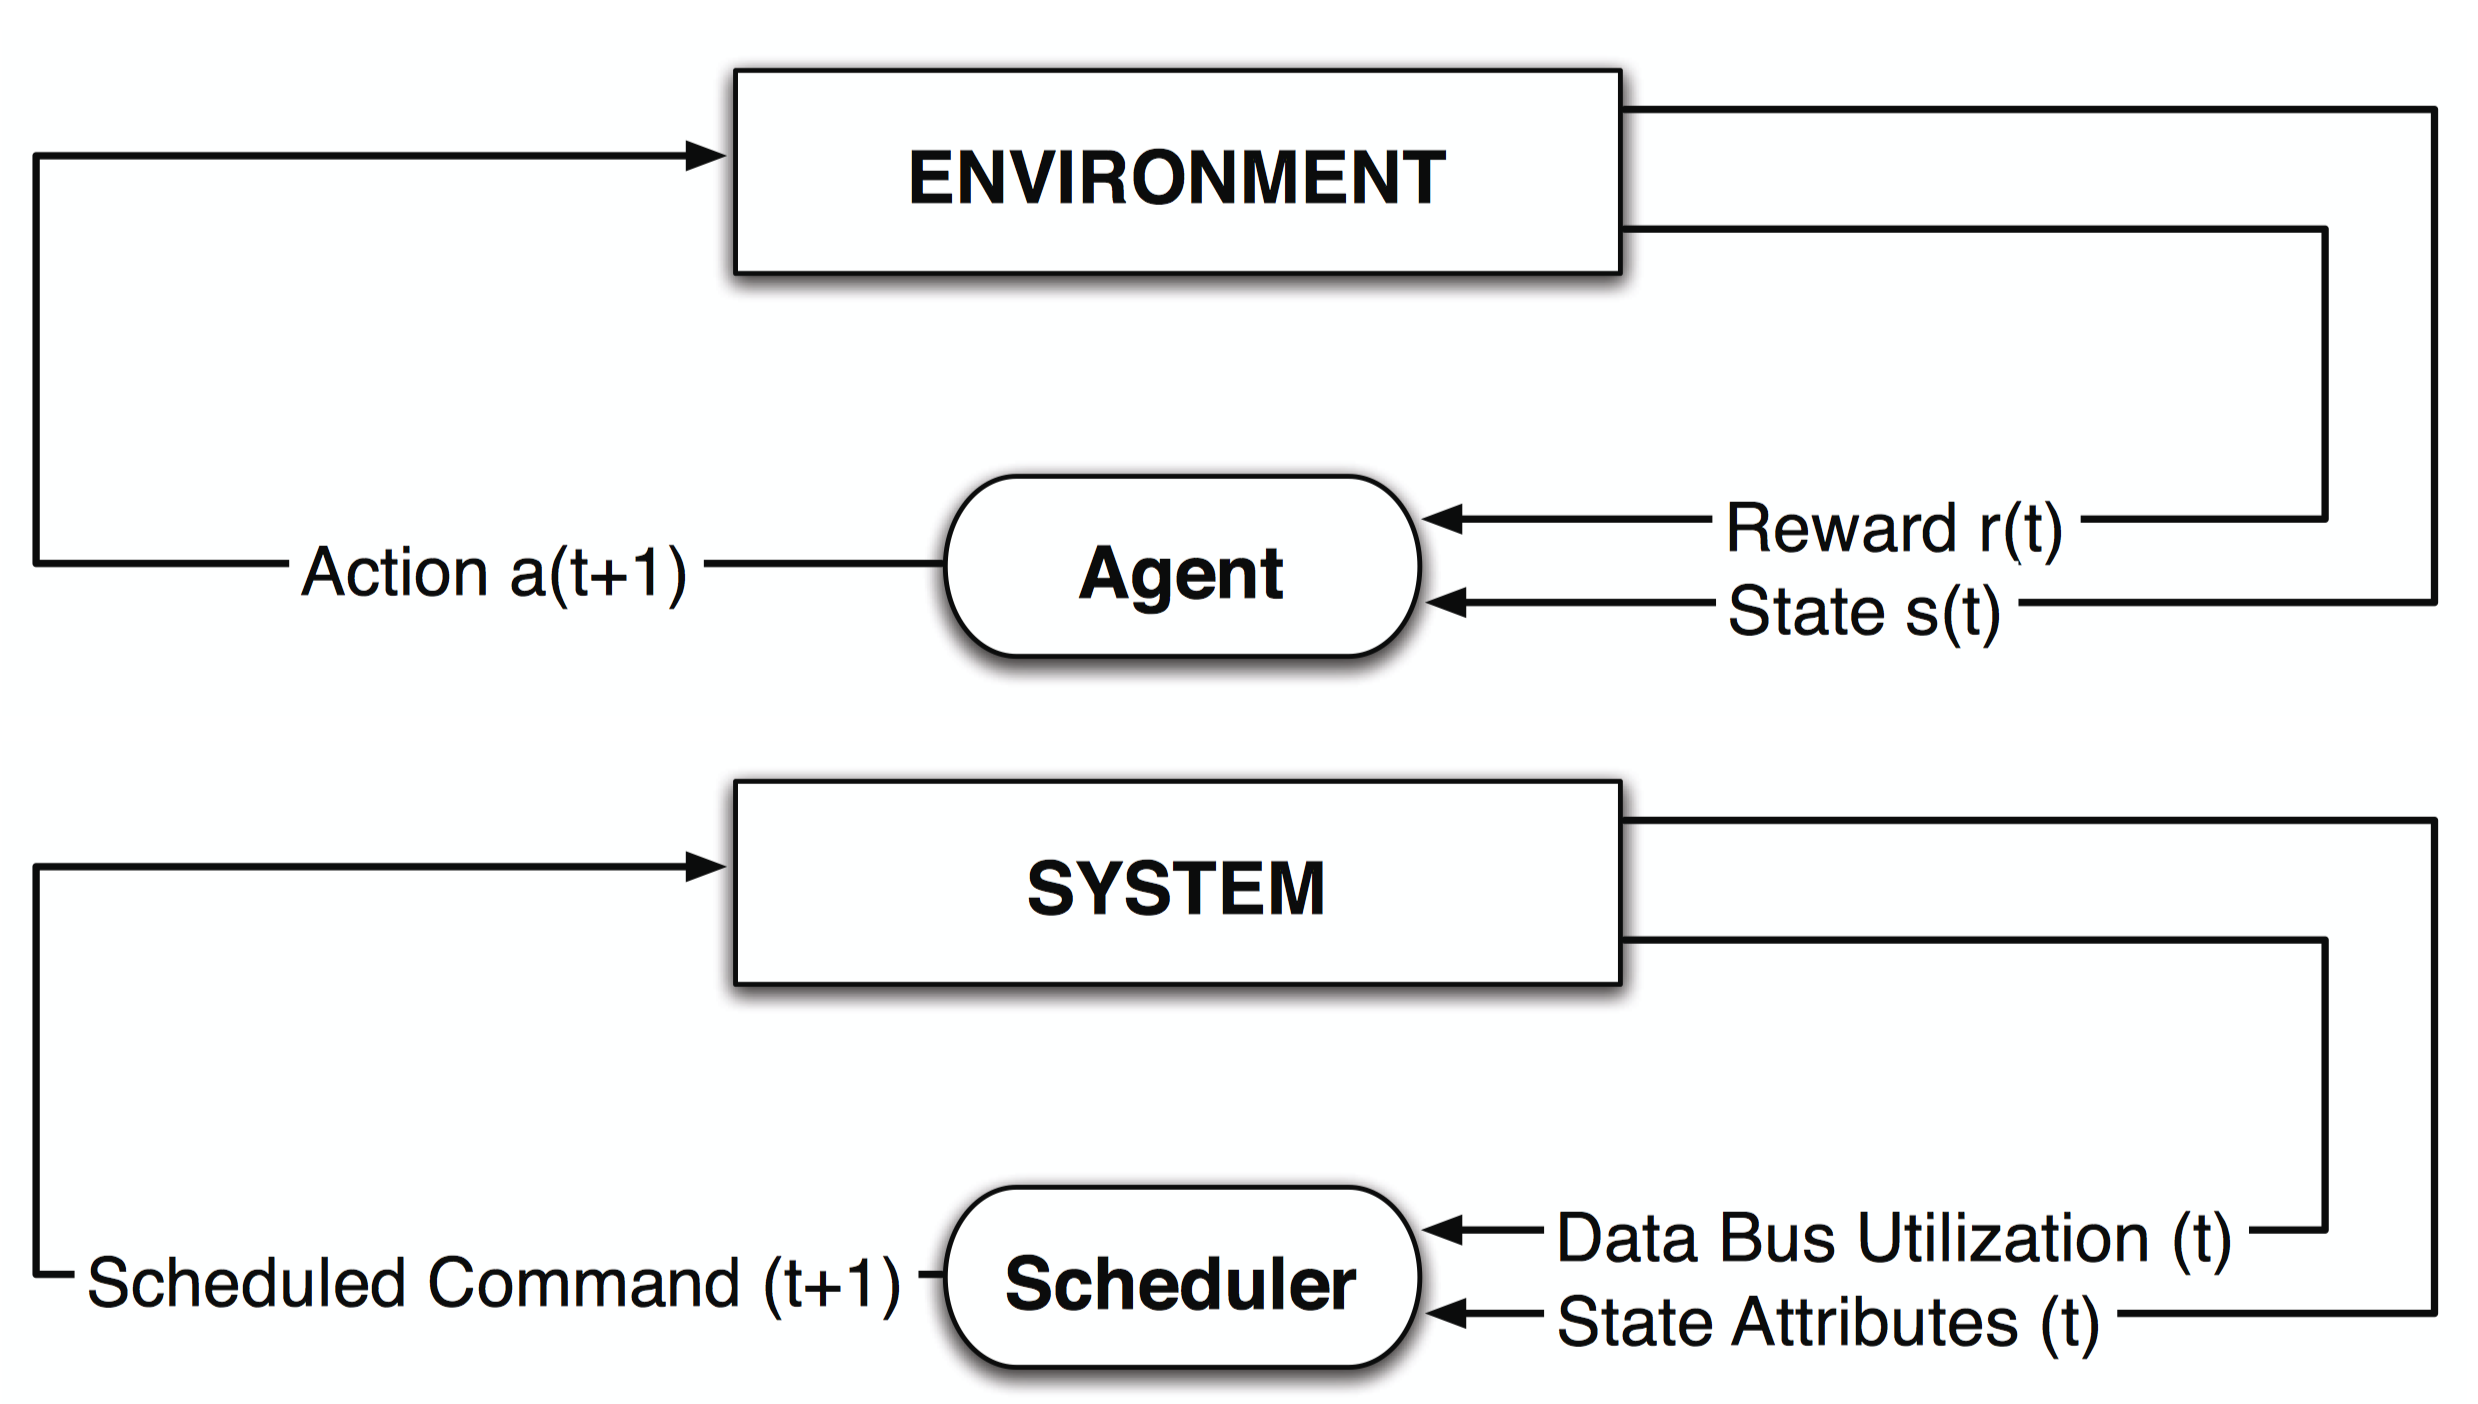
\includegraphics[width=1\linewidth]{rl/rl.png}
    \captionof{figure}{强化学习框架}
    \label{fig:rl}
  \end{minipage}     
\end{figure}


强化学习在一些极具挑战性的决策类优化问题中表现出其巨大潜力\cite{mnih2013playing}\cite{silver2016mastering}。强化学习中,智能体(agents)从过往的经验学习以做出更好的决策。图\ref{fig:rl}(a)展示了智能体如何与环境交互。交互过程被离散化成为一连串步骤,每一步智能体先感知环境的状态(state)为$s_t$,然后选择并执行一个动作(action)。这一步骤将导致环境的状态发生变化,转移至$s_{t+1}$,智能体在后续步骤中也将能够感知,此状态的变化还将生成一个奖励信号(reward)$r_t$。智能体对任务本身和规则一无所知,仅仅通过环境返回的奖励信号来的得知他当前学习到策略的好坏\cite{bertsekas1995dynamic}。智能体学习的目标时通过优化自身选择动作的策略,以最大化其累积奖赏。强化学习最近的研究将其和深度学习相结合,使得强化学习在很多应用上取得突破性的成绩,比如玩电子游戏\cite{mnih2015human},控制数据中心的冷却系统\cite{evans2016deepmind}等等。

回顾优化数据中心资源调度的问题,我们相信强化学习非常适合解决此类问题。首先,资源调度程序做出的决策通常有很高的重复性,因此可以产生大量数据用于强化学习训练。其次,正如我们在强化学习算法应用在游戏\cite{mnih2015human}\cite{evans2016deepmind}时看到的,强化学习算法可以通过深度神经网络(Deep Neural Network, DNN)模拟复杂的模型和决策过程。不同的信号和环境可能存在的轻微扰动都可以整合起来同时输入神经网络,产生一个决策模型。另外,通过强化学习,我们能够通过一个相关的奖励信号来优化一些难以直接优化的目标。最后,通过持续的学习,强化学习可以从大量经验中学到不同情况下的优化策略。

图\ref{fig:rl}(b)展示了如何在强化学习的框架内优化数据中心的资源调度以提高服务器利用率。智能体在这里充当资源调度器,而环境则包含了混合执行的延迟敏感型任务和批处理任务,支持这些任务的执行的所有服务器资源,以及按一定模式变化的延迟敏感型任务的负载。强化学习的每一步骤对应资源调度器的一次决策,智能体将在此时获得环境的状态并做出动作。环境相关的信息包括当前延迟敏感型任务的负载强度,计算核心,末级缓存和随机存储访存带宽等等资源的利用率,以及延迟敏感型任务的服务质量。智能体可做的选择则为增加分配给延迟敏感型任务的某类服务器资源,以提高其服务质量并避免违反服务质量要求,或是减少分配给延迟敏感型任务的某类资源以提高批处理任务性能并提高资源利用率。环境产生的奖励信号有多种设计目标。若此动作的执行导致资源敏感型任务违反其服务质量要求,智能体将给予惩罚(负的奖励);在不违反服务质量要求时,延迟敏感型任务占用的资源越少,智能体收到的奖励越大;所有的动作并不都一定可以在任意环境状态下执行,例如某类资源分配无法增加或减少,智能体若做出非法动作将会受到惩罚。

\section{强化学习在资源调度中的挑战}
将强化学习应用在数据中心的资源调度上时,同样面临挑战。首先是功劳分配问题(Temporal Credit Assignment),智能体需要学习如何从直接观察到的奖励信号中分析以前所执行的动作哪些有正面的贡献,哪些产生了负面的影响,以及这些负面的贡献和影响各有多大。在一些情况中,一些能立即产生高额奖励的动作可能将使系统进入不理想的状态,难以产生更多的奖励;而另一些情况中,一个动作可能无法产生立即的奖励,但可能对系统进入一个理想状态至关重要。因此最优的策略需要产生长远的规划,智能体需要能够预见未来的可能情况才能采取相应的行动以最大化总的奖励。其次是探索环境的积极性。智能体需要探索环境,学习不同状态下执行不同动作所带来的后果。一方面,积极的探索环境让智能体可能学会更高效的控制策略;另一方面,智能体在任何时刻也应该尽量执行已经找到的最优策略。对环境的探索太少将导致智能体始终执行没有足够优化的策略;而过多的探索将使智能体长时间执行不够优化的策略,拉长训练时间,且降低其性能表现。最后是泛化问题,环境的状态空间随考虑的因素指数增长,表示环境状态的变量可能相当大。在这种情况下,智能体很可能根本无法在此遇到以前经历过的环境状态。因此,从智能体的经验中学习并泛化是唯一可行办法。

\section{强化学习方法简介}
\subsection{马尔科夫决策过程(Markov Decision Processes, MDPs)}
考虑一般的强化学习场景,如图\ref{fig:rl}(a)所示,在每一步骤$\mathrm{t}$能观察到环境状态$\mathrm{s_t}$。当智能体执行动作$\mathrm{a_t}$后,环境状态变为$\mathrm{s_{t+1}}$,且智能体收到奖励$\mathrm{r_t}$。环境状态的转变和智能体收到的奖励都是随机的,并被假设具有马尔科夫性质(Markov Property)。因此,智能体所处的环境被抽象为马可夫决策过程(Markov Decision Processes,MDPs)。一个马尔科夫决策过程包含了一个状态集合$\mathbb{S}$,一个动作集合$\mathbb{A}$,一个状态间转换的关于动作的条件概率分布$\mathrm{T=\mathbb{P}(s_{t+1}=s'|s_t=s, a_t = a)}$,以及在每个状态下执行一个动作使得环境状态改变至另一个状态的奖励的期望$\mathrm{R=\mathbb{E}[r_{t+1}|s_t=s, a_t=a, s_{t+1}=s']}$。

\begin{figure}
  \centering
  \begin{minipage}[b]{0.7\textwidth}
    \centering
    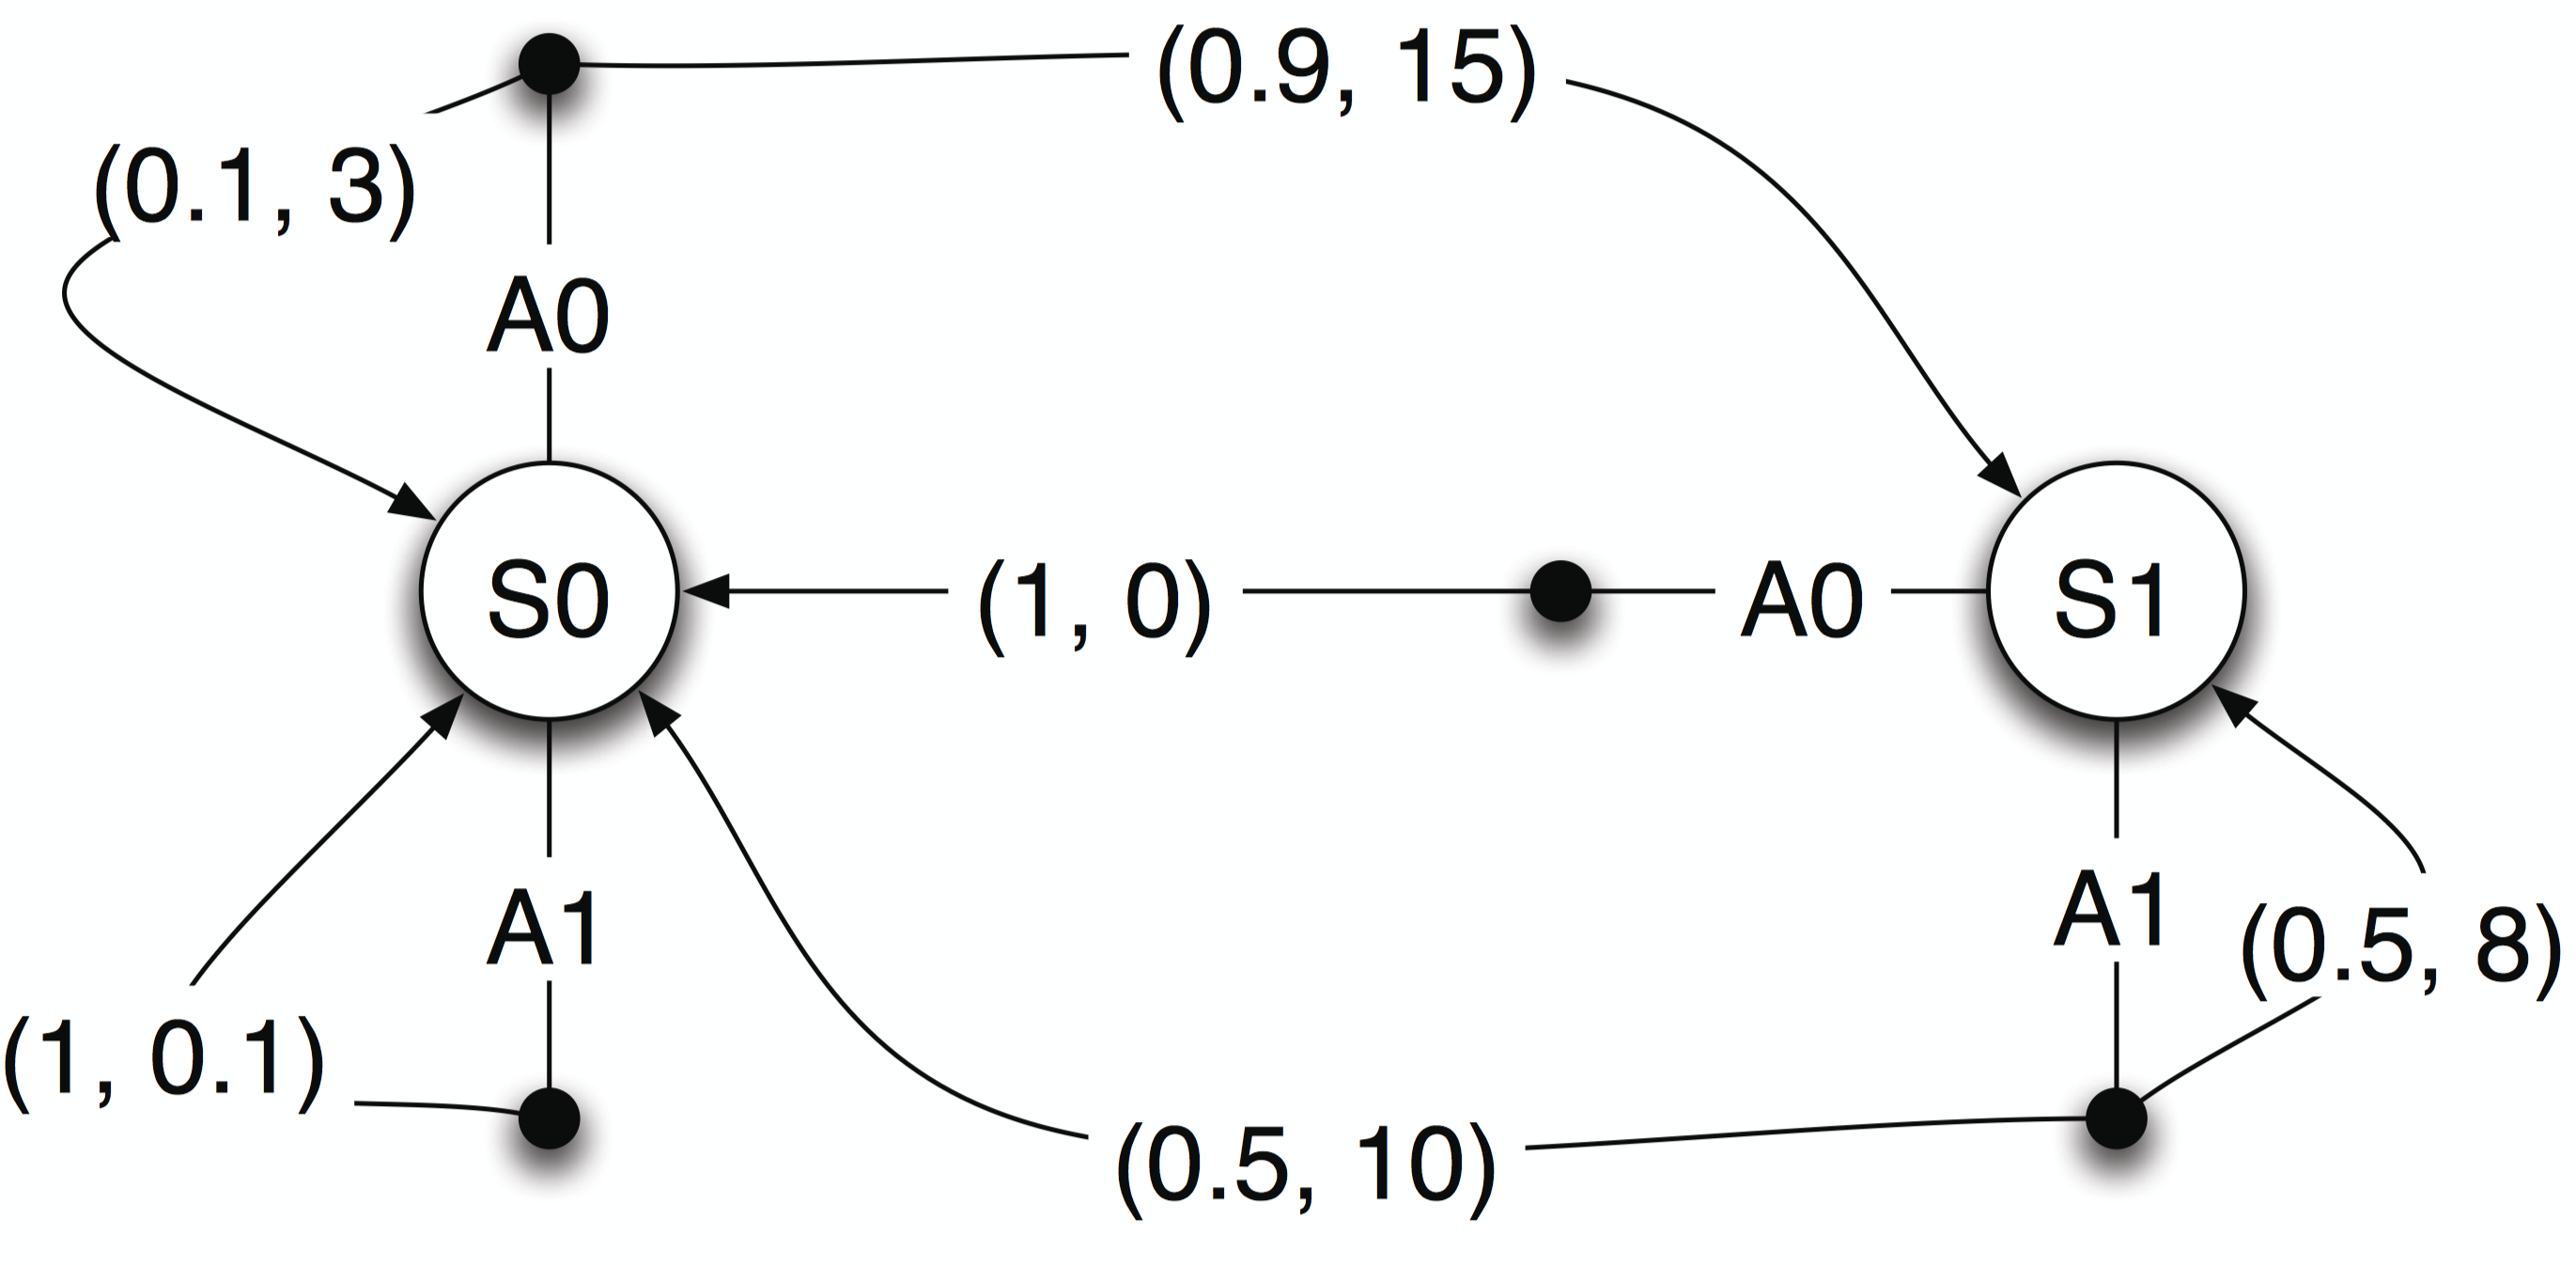
\includegraphics[width=1\linewidth]{rl/mdp.png}
    \captionof{figure}{马尔科夫决策过程示例}
    \label{fig:mdp}
  \end{minipage}     
\end{figure}

图\ref{fig:mdp}是一个马尔科夫决策过程的示例。示例的马尔科夫决策过程定义了两个环境状态$S0$和$S1$,和智能体在两个状态下都可选择执行的两个动作$A0$和$A1$。智能体在状态$S0$下执行动作$A0$,有$0.1$的可能性留在状态$S0$并获得$3$的奖励;同时有$0.9$的可能性转移至状态$S1$并获得$15$的奖励。智能体能控制的仅仅是选择下一个执行的动作,并且对环境可能的反应没有任何先验的知识。因此智能体的目标在于优化自身选择动作的策略以获得最大的累积奖赏。值得注意的是,对于智能体来说,执行某一动作后的状态转变并不总是确定的,有时是按概率跳转的。环境状态如何变化不在智能体的控制范围内,但智能体能通过大量的经验学习到其变化的规律。

用强化学习框架解决资源调度问题时,很自然会将总的步骤设为无限步骤,在无限长的时间里智能体通过合理分配服务器资源给延迟敏感型任务以保证其服务质量要求同时尽量提高服务器资源利用率。随着智能体考虑的时间由有限变为无限,一个潜在的问题是劣质的策略也能带来无限的总效用,导致智能体无法定义一个有效的优化目标。因此,在无限时间步骤时,优化折现后的累计奖赏(discounted cumulative reward)更为合适,这可以理解为如果能拿到奖赏,智能体倾向于尽早拿到奖赏。同时,由于智能体的优化目标仍然是累积奖赏,因此智能体仍然有发现远期更高价值奖赏的潜力。折现累积奖赏可表示为\ref{eq:discounted_reward},其意义为当前步骤后执行$i$次动作后得到奖赏的期望$r_{t+i}$在当前决策中的价值为$\gamma^i*r_{t+i}$,其中$\gamma$为折现率。

\begin{equation}
  \label{eq:discounted_reward}
    R = \mathbb{E}(\sum_{i=1}^{\infty} {\gamma^{i}} \cdot r_{t+i})
\end{equation}

\subsection{策略与状态值函数}
强化学习中智能体根据其学习到的策略和观察到的环境状态选择下一执行动作。策略是一个关于动作的条件概率$\pi: \pi(s, a)\rightarrow[0,1]$。$\pi(s, a)$表示了智能体在环境状态为$s$时选择执行动作$a$。当考虑的环境因素增加时,环境状态的可能情况呈指数上升。一般具有时间研究意义的问题都考虑较多的环境变量导致环境状态空间巨大。这种情况下,智能体学习的策略无法用传统的表格方式表示,而需要用一个函数来近似\cite{bertsekas1995dynamic}\cite{menache2005basis}。通过函数近似,我们可以用可接受数目的参数$\theta$来近似策略$\pi(s, a)$,我们将通过参数$\theta$来参数化近似表示的策略记为$\pi_\theta(s,a)$。函数近似可以解决问题的一个理由是对于相似的状态,我们认为智能体本来也应该采取相同的动作以优化其目标。

很多函数近似方法都可以用来实现近似强化学习中的策略函数,例如通过环境状态和动作空间的特征进行线性组合来近似策略$\pi(s,a)\approx\pi_\theta(s,a)=\theta^T\phi(s,a)$。 深度神经网络在最近的研究中被用作函数近似来表示策略函数,并在一些大规模的强化学习场景中取得很好效果。使用深度神经网络而不是前文提到的特征的线性组合的一个优点是不需要繁琐的特征工程来选取环境状态和动作中的特征。图\ref{fig:policy}表示了如何使用深度神经网络来近似策略函数时进行强化学习。

\begin{figure}
  \centering
    \centering
    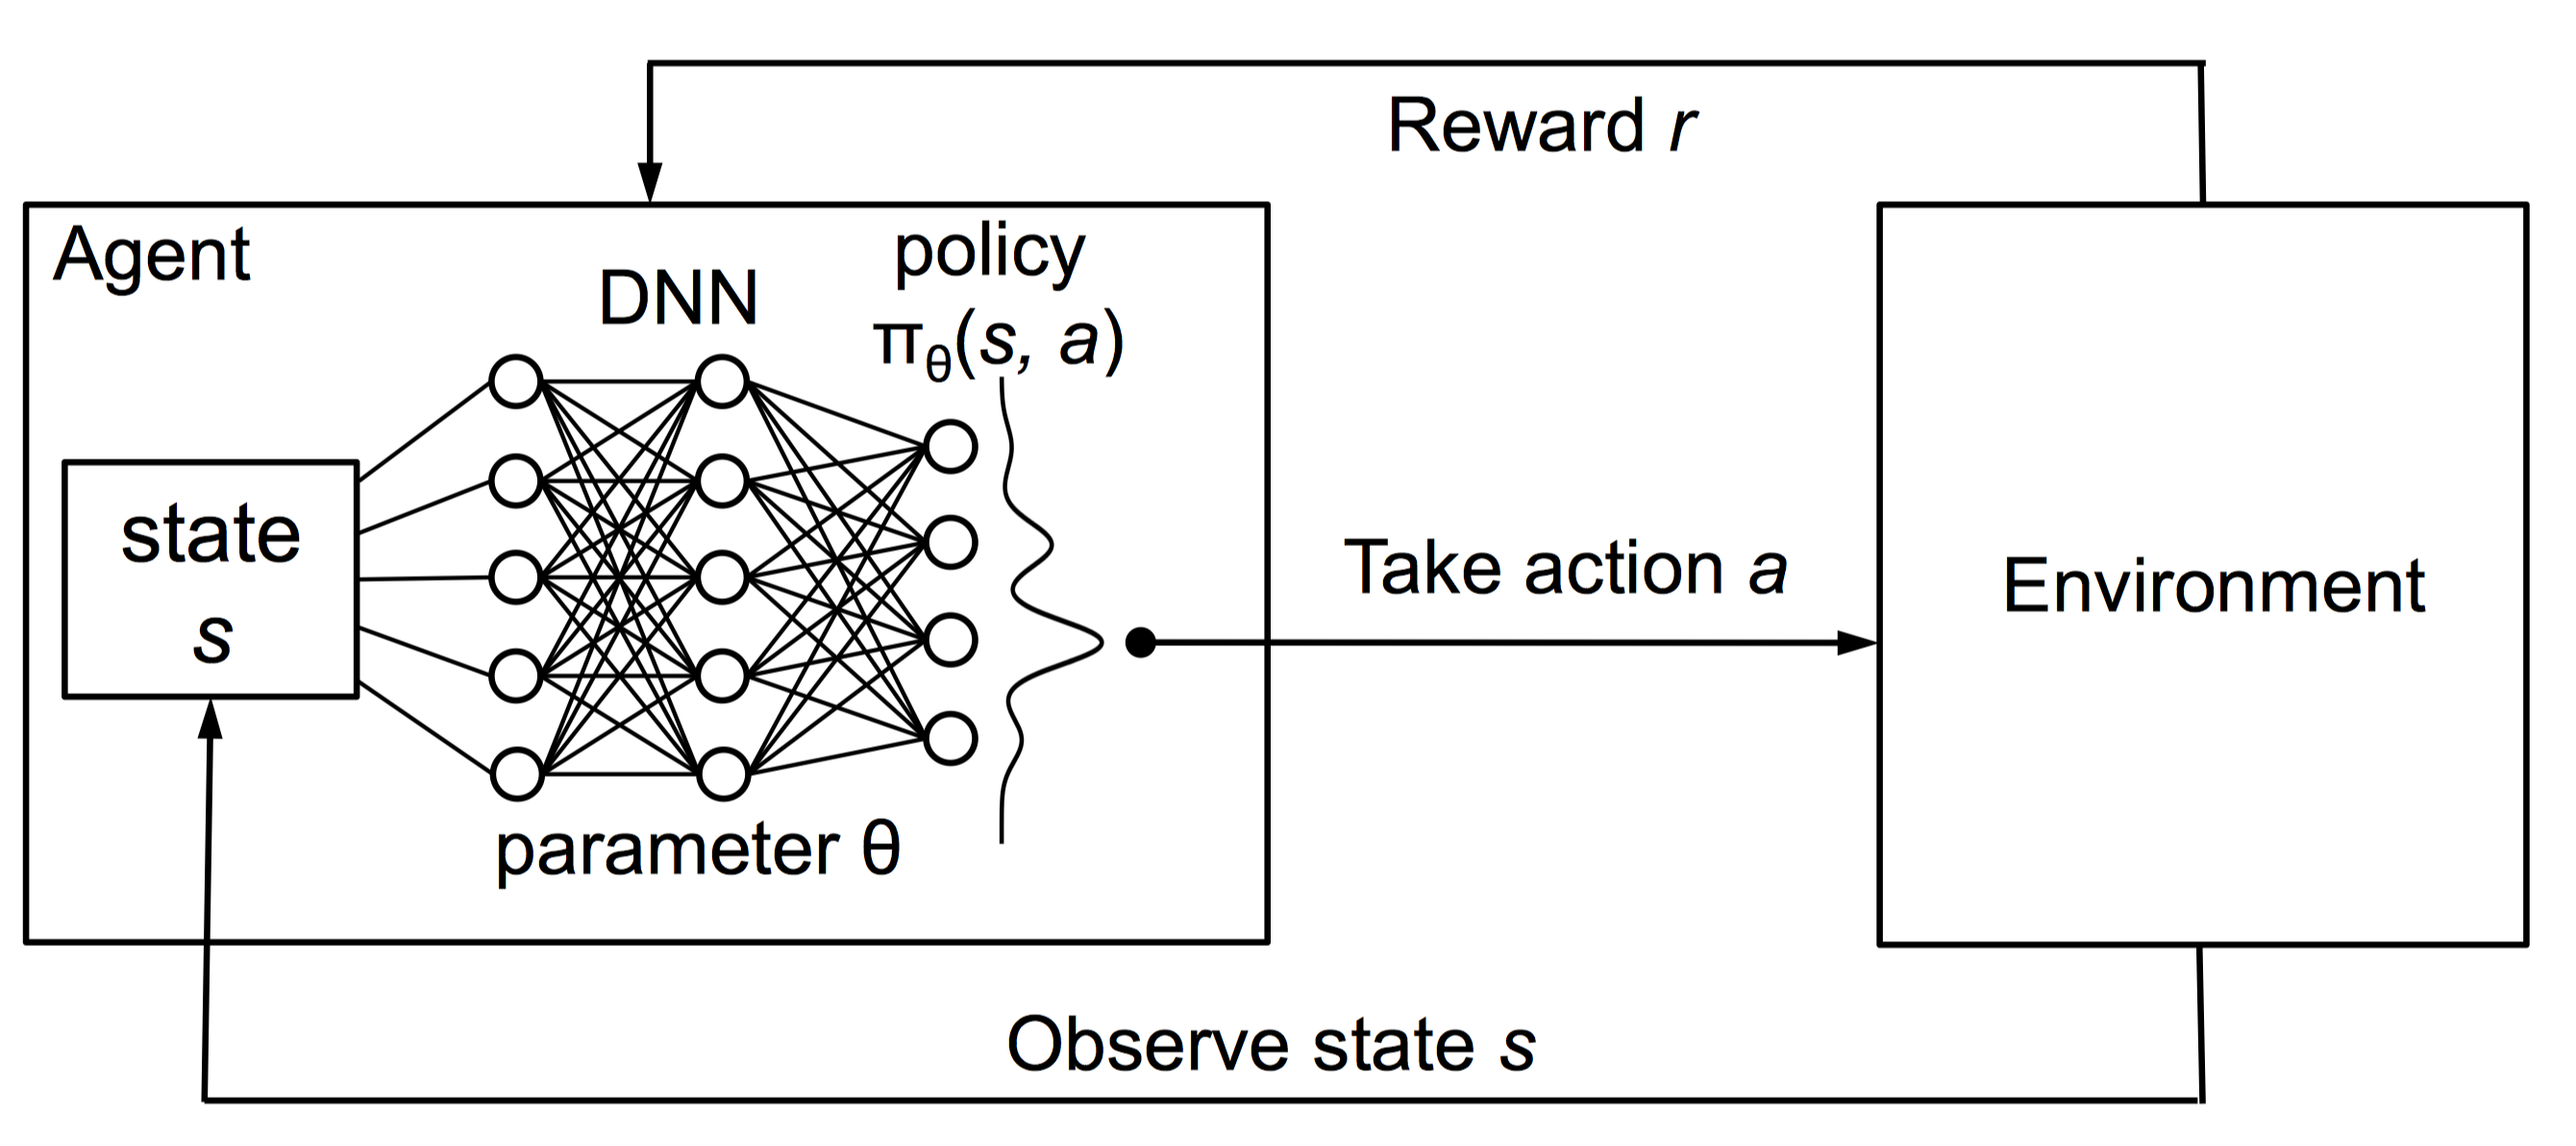
\includegraphics[width=1\linewidth]{rl/policy.png}
    \captionof{figure}{通过深度神经网络近似策略函数}
    \label{fig:policy}    
\end{figure}

当智能体按照一个给定的策略选择动作并执行时会产生一系列的环境状态,执行动作和奖赏信号的序列,如$s_0, a_0, r_0,s_1, a_1, r_1 ...$。状态值函数(Value Function),见式\ref{eq:val_func},$V^{\pi_\theta}(s)$表示了从指定的环境状态$s$开始,执行按照策略$\pi_\theta$产生的动作序列,可获得的折现后累积奖赏的期望。我们将状态值函数,作为判断一个环境状态好坏的标准。

\begin{equation}
  \label{eq:val_func}
  	V^{\pi_\theta}(s)=\mathbb{E}_{\pi_\theta}\bigg[\sum_{t=0}^{\infty} {\gamma^{t}} \cdot r_{t}|s_0=s\bigg]
\end{equation}

进一步的,我们还定义Q值函数(Q-value Function)来作为判断一个环境状态/动作对的好坏的标准,见式\ref{eq:qval_func}。Q值函数$Q^{\pi_\theta}(s,a)$从指定的环境状态$s$开始,在执行动作$a$后,所有的后续动作完全按照策略$\pi_\theta$产生的动作执行,可以得到的折现后累积奖赏的期望。Q值函数可以用来解决前文所提到的功劳分配问题\cite{michalski2013machine}\cite{sutton1998reinforcement},从下一节策略梯度方法中的式\ref{eq:gradient}可以看到值函数与Q值函数之间密切的关系。

\begin{equation}
  \label{eq:qval_func}
  	Q^{\pi_\theta}(s,a)=\mathbb{E}_{\pi_\theta}\bigg[\sum_{t=0}^{\infty} {\gamma^{t}} \cdot r_{t}|s_0=s, a_0=a\bigg]
\end{equation}

在大规模的问题中,环境状态的空间远远大于我们可以用表格值来精确表示的规模。

\subsection{策略梯度方法(Policy Gradient Methods)}

智能体优化策略的一个算法是通过计算值函数的策略梯度,并按计算的梯度调整策略实现最大化值函数,也就是最大化从当前状态开始的折现累积奖赏的期望。我们的优化目标是式\ref{eq:discounted_reward}给出的折现累积奖赏,其梯度表示为式\ref{eq:gradient}\cite{sutton1998reinforcement}。

\begin{equation}
  \label{eq:gradient}
  	\nabla_{\theta}\mathbb{E}_{\pi_\theta}\bigg[\sum_{t=0}^{\infty} {\gamma^{t}} \cdot r_{t}\bigg]= \mathbb{E}_{\pi_\theta}\big[\nabla_\theta\operatorname{log}\pi_\theta(s,a)Q^{\pi_\theta}(s,a) \big]
\end{equation}

其中$Q^{\pi_\theta}(s,a)$是在状态$s$是执行动作$a$并在后续均按$\pi_\theta$的策略选择所有动作时得到的折现后累积奖赏。策略梯度的主要思想是通过按照策略执行动作并观测环境的变化来估计环境变化随策略的变化,并由此计算策略梯度。这本质上是一个简单的蒙特卡罗方法\cite{hastings1970monte}——智能体通过采样多种动作执行的序列和环境状态的变化序列获得经验,然后根据这些经验来计算折现累积奖赏$v_t$,并将其作为对$Q^{\pi_\theta}(s,a)$的无偏估计,即$v_t = \hat{Q}^{\pi_\theta}(s,a)$ 。然后,智能体根据估计出的策略梯度来更新现有策略以求优化折现累积奖赏\cite{sutton2000policy},见式\ref{eq:update}。其中$\alpha$是学习率。
\begin{equation}
  \label{eq:update}
  \theta \leftarrow \theta + \alpha\sum_{t}{}\nabla_{\theta}\operatorname{log}\pi_{\theta}(s_t, a_t)\dotv_t
\end{equation}

梯度$\nabla_{\theta}\operatorname{log}\pi_{\theta}(s_t, a_t)$给出了通过改变近似策略的参数$\theta$来增加$\pi_{\theta}(s_t, a_t)$(即在状态$s_t$下,策略选择执行动作$a_t$的概率)的方向。而应该多大程度地将策略向此方向调整(即多大程度地增加策略在状态$s_t$下,策略选择执行动作$a_t$的概率),取决于智能体当前对于$Q^{\pi_\theta}(s,a)$的无偏估计$v_t$。如果当前智能体通过经验估计到的$v_t$越大,即智能体认为在后获得的累积折现奖赏越大,智能体就将越积极的调整策略,使得学习到的策略在状态$s_t$下有更大的可能性执行动作$a_t$。若智能体通过经验估计到的$v_t$越小,则智能体将会越不愿意在状态$s_t$下执行动作$a_t$,因此更新后的策略在状态$s_t$下选择动作$a_t$的可能性增加将会较少;在$v_t$为负值的情况下,策略在状态$s_t$下选择动作$a_t$的可能性还将降低。

\subsection{Q学习(Q-learning)}
最优的Q值函数$Q^*(s,a)$是通过改变策略参数$\theta$,从指定的环境状态$s$,执行动作$a$后,按照策略$\pi_\theta$产生的动作序列执行,可获得最大期望折现后累积奖赏。
\begin{equation}
  \label{eq:q_opt}
    Q^*(s, a) = \underset{\theta}{\mathrm{max}}\,Q^{\pi_\theta}(s,a)=\underset{\theta}{\mathrm{max}}\,\mathbb{E}_{\pi_\theta}\bigg[\sum_{t=0}^{\infty} {\gamma^{t}} \cdot r_{t}|s_0=s, a_0=a\bigg]
\end{equation}

最优Q值函数满足以下的Bellman等式\ref{eq:bellman}。直觉上容易理解,如果已知最优Q值函数,那么只需要在下一状态选择选择执行使Q值函数最大的动作即可最大化折现的累计奖赏的期望。
\begin{equation}
  \label{eq:bellman}
    Q^*(s, a) = \mathbb{E}_{s' \sim \mathbb{P}}\big[r(s,a,s') + \gamma\cdot \underset{a'}{\mathrm{max}}\,Q^*(s',a') |s_0=s, a_0=a\big]
\end{equation}
学习最优的Q值函数$Q^*(s,a)$,则等同于学习最优的策略$\pi_\theta(s,a)$,Q学习通过动态规划,多次迭代来学习最优Q值函数,如式\ref{eq:q_learning}。容易看到,$\lim_{i\to\infty} Q_i = Q^* $。

\begin{equation}
  \label{eq:q_learning}
    Q_{i+1}(s, a) = \mathbb{E}_{s' \sim \mathbb{P}}\big[r(s,a,s') + \gamma\cdot \underset{a'}{\mathrm{max}}\,Q_i(s',a') |s_0=s, a_0=a\big]
\end{equation}

与策略的神经网络参数化表示相同,我们同样可以通过深度神经网络来近似Q值函数。

\subsection{Actor-Critic}
策略梯度方法存在的一个问题是其训练结果的方差过大。如果我们通过设置基准$b$来减小模型的方差,如\ref{eq:gradient_baseline}。
\begin{equation}
  \label{eq:gradient_baseline}
    \nabla_{\theta}\mathbb{E}_{\pi_\theta}\bigg[\sum_{t=0}^{\infty} {\gamma^{t}} \cdot r_{t}\bigg]= \mathbb{E}_{\pi_\theta}\big[\nabla_\theta\operatorname{log}\pi_\theta(s,a)(Q^{\pi_\theta}(s,a)-b) \big]
\end{equation}
更进一步,当使用状态值函数作为基准时,策略梯度为\ref{eq:gradient}将变为\ref{eq:gradient_advantage}。
\begin{equation}
  \label{eq:gradient_advantage}
    \nabla_{\theta}\mathbb{E}_{\pi_\theta}\bigg[\sum_{t=0}^{\infty} {\gamma^{t}} \cdot r_{t}\bigg]= \mathbb{E}_{\pi_\theta}\big[\nabla_\theta\operatorname{log}\pi_\theta(s,a)(Q^{\pi_\theta}(s,a)-V^{\pi_\theta}(s)) \big]
\end{equation}
其中$Q^{\pi_\theta}(s,a)-V(s))$被称为动作优势函数$A(s,t)$(Advantage Function)。如果不考虑状态转移的概率,使用采样的方式来估计状态转移,则在当前的策略参数下Q值函数可以近似为式\ref{eq:q_approx}:
\begin{equation}
  \label{eq:q_approx}
   Q^{\pi_\theta}(s_t, a_t) \approx r^{\pi_\theta}(s_t, a_t) + V^{\pi_\theta}(s_{t+1})
\end{equation}
根据此近似,式\ref{eq:gradient_advantage}简化为式\ref{eq:gradient_advantage_approx},通过此近似进行策略梯度学习需要通过采样对状态值函数进行估计。与策略一样,状态值函数同样可以使用深度神经网路近似。此时,选择动作的策略网络被称为动作执行者(Actor),而对状态进行评价的状态值函数被称为评委(Critic)。训练算法可以简单描述为,Actor执行多个动作,Critic通过观察Actor各个动作和环境的变化来改变自己对环境状态的评价;同时Actor根据Critic对环境状态的评价来产生策略梯度,由此改变自身动作选择的策略。
\begin{equation}
  \label{eq:gradient_advantage_approx}
    \nabla_{\theta}\mathbb{E}_{\pi_\theta}\bigg[\sum_{t=0}^{\infty} {\gamma^{t}} \cdot r_{t}\bigg]= \mathbb{E}_{\pi_\theta}\big[\nabla_\theta\operatorname{log}\pi_\theta(s,a)(r^{\pi_\theta}(s_t, a_t) + V^{\pi_\theta}(s_{t+1})-V^{\pi_\theta}(s)) \big]
\end{equation}

等价的,根据式\ref{eq:q_approx}中所做的近似,式\ref{eq:gradient_advantage}同样可以简化为式\ref{eq:gradient_q_approx},此时可以通过估计Q值函数替代估计状态值函数。

\begin{equation}
  \label{eq:gradient_q_approx}
    \nabla_{\theta}\mathbb{E}_{\pi_\theta}\bigg[\sum_{t=0}^{\infty} {\gamma^{t}} \cdot r_{t}\bigg]= \mathbb{E}_{\pi_\theta}\big[\nabla_\theta\operatorname{log}\pi_\theta(s,a)(r^{\pi_\theta}(s_t, a_t) + Q^{\pi_\theta}(s_t, a_t)-Q^{\pi_\theta}(s_{t-1}, a_{t-1})) \big]
\end{equation}




% $Q(s,a;\theta) \approx Q*(s,a)$。David Silver等人提出训练深度Q网络(Deep Q-Network)的方法\cite{mnih2015human}。相比于普通的在线Q学习方法,他们提出经验重放(Experience Replay)和双重Q网络训练的方法。经验重放即智能体将记住曾经做过的动作和导致的结果,并在将来回忆。经验重放使得一次采样多次用于神经网络的训练,提高了数据的利用率;同时,他避免了通过具有高关联性的连续样本训练的低效率问题。双重Q网络的应用也降低了训练过程中的震荡问题。具体的算法和其在本问题中的应用将在实验部分介绍。
% \subsection{}
% from policy gradient to Q leaning






% graph
\chapter{实验环境}
\section{模型设计}
考虑在具有多种可调度资源的单个服务器上混合执行延迟敏感型任务和批处理任务的问题。智能体执行调度的周期可设置为足够小,以至于在每个时间步骤内,延迟敏感型任务的负载可视为基本不发生变化。通过调度决策开始时到延迟敏感型应用的请求数量,可以预计此段时间步骤内延迟敏感型任务的负载强度。根据预计的负载强度和当前服务器的各类资源利用率(环境状态),智能体选择动作进行资源调度。在当前周期结束后,智能体将收到新的预计负载强度和新的服务器资源利用率。同时,智能体还会收到反映上一个动作质量的奖励信号。

智能体的优化目标是在不违反延迟敏感型任务的服务质量要求的同时,优化服务器的资源利用率。当我们假设批处理任务可以充分利用被分配的资源时,一个相关的且容易量化的优化目标为分配给延迟敏感型任务的资源尽量少。上述假设通常是成立的。

\subsection{隔离技术}
\textbf{计算核心资源}直接影响任务获得的计算速度和并行计算能力。通过Linux系统提供的cgroup,我们可以任意为延迟敏感型任务和批处理任务分配计算核心。实验在英特尔Xeon(R
) E5-2630上进行。该处理器具有10个物理计算核心,20个逻辑计算核心。英特尔的超线程技术使得共用同一个物理计算核心的超线程将共用一二级高速缓存。而对于非末级高速缓存的访问目前没有办法进行隔离,因此我们将资源分配的粒度设置为分配物理核心以防止批处理任务与延迟敏感型任务在同一物理核心上运行时在一二级高速缓存上产生干扰。\textbf{末级高速缓存}上批处理任务对延迟敏感型任务在延迟敏感型任务高负载强度时产生巨大的干扰。因此隔离任务对末级高速缓存的使用能有效保证延迟敏感型任务在高负载强度时的服务质量。处理器硬件提供20级的缓存分配,为简化问题,我们将缓存分配设置为10级,即资源分配的粒度为末级高速缓存总大小的十分之一。用于控制\textbf{动态随机存储访问带宽}的内存带宽分配技术(MBA)在实验环境的服务器上缺乏硬件支持,因此无法直接控制混合执行任务对动态随机存储器的访问。
用于替代内存带宽分配技术,我们一般通过内存带宽监控技术(MBM)检测每个计算核心产生的动态随机存储访问流量,当批处理任务对动态随机存储访问带宽产生过大压力时,减少分配给批处理任务的计算核心以降低其对动态随机存储的访问,然而从后续一节\nameref{sec:pref_analysic}中发现,这种粗粒度的调节并不能取得很好效果。

\begin{figure}
  \centering
    \centering
    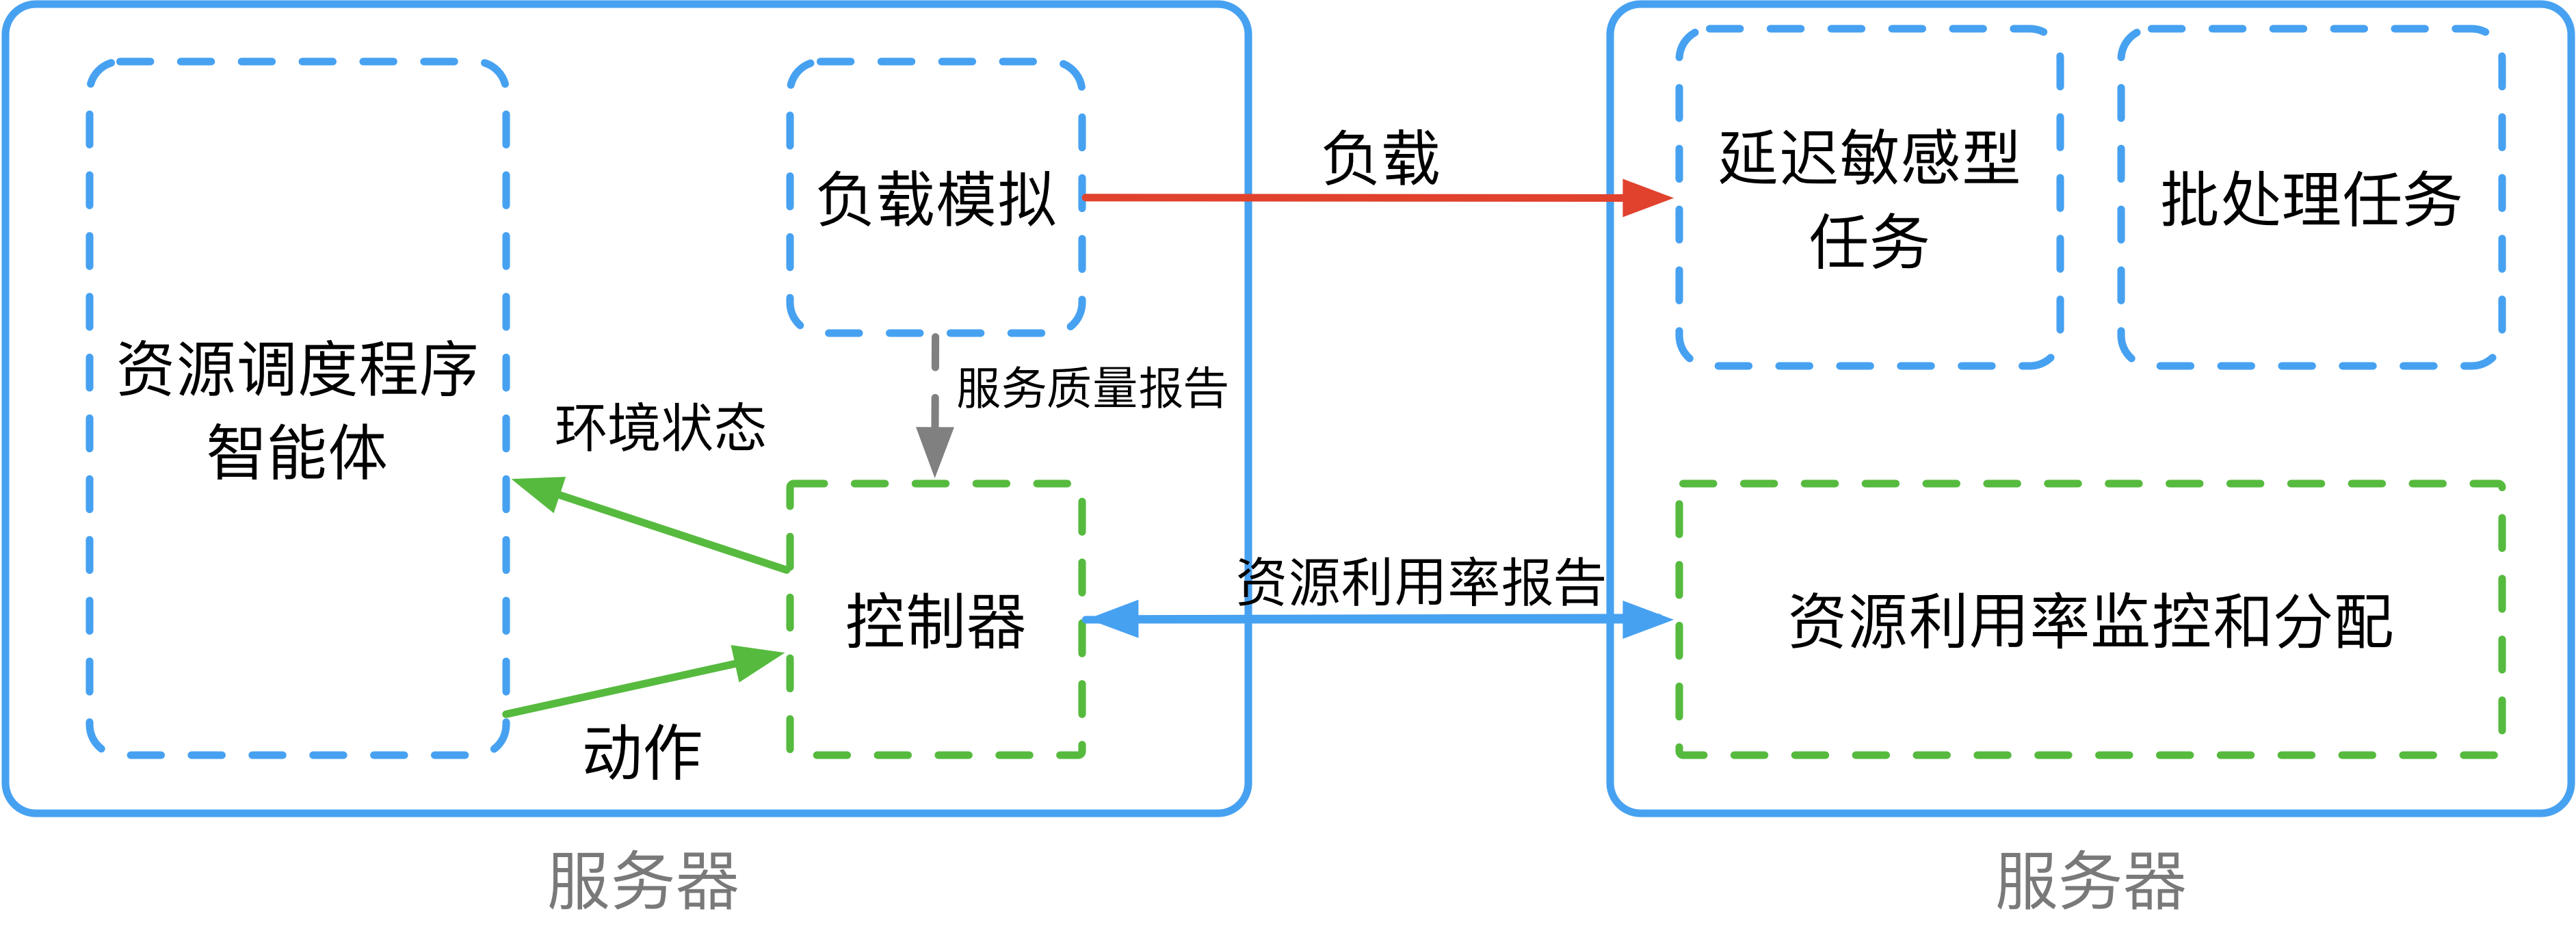
\includegraphics[width=0.9\linewidth]{exp/overview.png}
    \captionof{figure}{实验系统架构}
    \label{fig:overview}    
\end{figure}

\subsection{整体架构}
为避免资源调度算法与延迟敏感型程序抢夺资源,资源调度程序将在单独的硬件上运行,并通过与延迟敏感型程序混合执行的一个轻量控制程序监控资源利用和进行资源调度。系统的整体架构如图\ref{fig:overview}所示。

充当资源调度程序的智能体通过与其运行在同一服务器上的控制器与环境交互。当只能体做出动作时,控制器接受智能体的动作,并将其传递至被调度服务器上执行。被调度的服务器上运行的轻量控制器将在指定的时间内取样服务器的资源利用率并返回给调度程序端的控制器。除了执行来自智能体的动作,控制器还将调动负载模拟程序向延迟敏感型任务施加负载并收回此段时间内的服务质量报告。为了获得具有统计学意义的数据,以上施加负载和采样资源利用率的过程都被设定为足够长以允许延迟敏感型任务服务足够多的请求。所有搜集到的数据,包括资源利用率报告和服务质量报告,将作为环境状态和计算出的此步骤奖励一起返回给资源调度智能体。

\section{混合执行任务选择}
\subsection{延迟敏感型任务}
数据中心常见的延迟敏感型任务包括社交网络,搜索引擎,软件即服务,在线地图,网页邮箱,机器翻译,在线购物和广告等等。

\subsubsection{Elgg 社交服务引擎}\lable{sec:elgg}
社交网络应用与普通网站服务不同,其更多是一个平台。例如脸书(Facebook)就给用户提供了一个社交平台。社交网络上的大部分数据是由用户(而不是开发者)产生。这些数据由其他用户的行为,或外来资源的变化而引起动态更新,并被推送给用户。正因为如此,社交网络应用包含频繁的后端数据库写入,且写入的数据将在后来推送给用户。

Elgg社交服务引擎是一个基于PHP实现的开源社交网络应用,并被包括澳大利亚政府,新西兰教育部,Wiley出版社,弗罗里达大学在内的机构使用\cite{palit2016demystifying}。Elgg社交服务引擎提供与流行的社交服务脸书提供相似的功能,允许用户在其中建立一个个人好友网络,并在网络中互相分享内容。Elgg社交引擎还包括一个迷你博客Elgg Wire,可用于与其他用户分享文字,图片和视频内容。在Elgg Wire中分享的内容被其他用户可见,类似与脸书中发文上墙的功能。每一个用户都有自己的实时与好友网络共享的信息流,被称为Elgg River。通过Elgg,用户可以实现多种操作,比如发送和接收聊天信息,在Elgg Wire上发送动态,以及接收其他用户最新分享的内容。所有的操作都有AJAX发送和接受简短消息实现,因此Elgg的主要负载都是这些来自AJAX的简短请求。

Elgg的后端通过服务器脚本语言PHP和MySQL数据库实现。脸书的服务器后端相似\cite{nishtala2013scaling},我们还通过Memcached加速数据库访问。为了简化问题,Elgg的网页服务器和后端,包括MySQL和Memcached都运行在同一服务器上,并作为延迟敏感型任务分配资源。

我们使用Faban框架来实现Elgg社交引擎的服务质量测试。Faban是一个基于Java的基准测试开发和执行框架,提供了API用于快速开发基准测试程序。通过定义测试的操作和各种操作的执行概率,可以快速开发网络应用的基准测试。在基准测试完成后,Faban将输出各个操作执行情况的统计数据,例如执行测试,相应时间和违反服务质量要求的情况。

Elgg提供了多种功能,因此用户可以进行多种操作,例如登录登出,添加好友,发送接收消息和分享动态等。考虑到真实用户执行不同操作具有不同频率,且每一个操作与前一个操作具有一定关联,我们通过一个马尔科夫过程(Markov Process)模拟用户的行为。Elgg的服务质量被定义为一段时间内所有该操作的响应时间的九十分位点。从服务器来看,模拟用户总体的产生的各个操作的比例各个操作和其服务质量要求如表\ref{tab:mix}所示。对于Elgg引擎服务质量的设置参考于Facebook各操作的平均延迟\cite{alexa2016},对于注册、登录和退出等用户不频繁使用的的操作,设置了较低的服务质量要求。

\begin{table}[!htp]
  \centering
  \captionof{table}{模拟用户总体访问模式}\label{tab:mix}
  \begin{tabular}{@{}lcc|lcc|lcc@{}} \toprule
    操作 & 占比 & 服务质量要求 & 操作 & 占比 & 服务质量要求 & 操作 & 占比 & 服务质量要求\\ 
    \midrule
    注册 & 0.5 & 3 & 首页 & 5 & 1 & 发消息 & 17 & 1 \\
    登录 & 2.5 & 3 & 动态 & 20 & 1 & 收消息 & 17 & 1 \\
    退出 & 2.5 & 3 & 好友 & 10 & 1 & 刷新主页 & 25.5 & 1\\
    \bottomrule
  \end{tabular}  
\end{table}

\subsubsection{对象缓存服务}
为了提高性能,网络应用通常使用对象缓存服务(Object Caching)来缓存一些代价昂贵的操作的计算结果,因此对象缓存服务存储和读取的速度将极大影响整个服务的性能。Memcached是一个常用的以键—值形式存储的对象缓存系统,通常用来缓存一些用时较长的数据库请求的结果。对网页服务器的一个请求一般会使网络服务器产生多个对对象缓存服务的请求。为了避免网页加载的延迟,对象存储服务必须以低延迟返回请求结果,因此其服务质量(九十分位延迟)通常设置在十毫秒。

Cloudsuit中提供了Memcached的基准测试程序Memloader\cite{palit2016demystifying}。由于对象缓存服务的请求基本无需额外的处理,因此对象缓存服务器除了低延迟外,还具有很高吞吐量。Memloader对此优化了基准测试程序结构。测试程序通过C++实现以提高性能,在其产生的多个测试线程中,一半的线程进行请求,另一边的线程验证缓存服务返回的信息。两种线程的分工减少了请求和处理间的干扰,有利于准确计时和产生统计信息。由于Memcached已知的规模扩展问题,即当其产生超过四个线程时会由显著性能下降,因此实践中一般在一个服务器上运行多个Memcached实例。Memloader可以在多个缓存服务器之间平衡负载。测试结束后,基准测试可以报告平均的请求延迟,九十分位延迟和缓存命中率等数据。

Memcached的高吞吐量使得缓存服务器和运行基准测试的服务器之间的网络连接成为性能瓶颈,通常要求其间的连接带宽在10Gbps以上。实验环境中不具备这样的网络连接条件,为避免网络瓶颈,我们在具有多个处理器接口的服务器上,每个接口分别运行对象缓存服务和基准测试程序,以利用系统中高速的网络回路连接(loopback)。

\subsection{批处理任务}
数据中心存在多种批处理任务,例如文件备份,离线图片处理和视频转码压缩等。来自普林斯顿大学的测试程序套装(Princeton Application Repository for Shared-Memory Computer, PARSEC)\cite{bienia11benchmarking}包含了一些典型的数据中心批处理任务。

\subsubsection{视频编码}
随着存储和网络带宽的增加,网络视频在网络流量中占比显著增加,视频的解码,转码,压缩等任务对于如Youtube的视频网站十分重要。视频编码测试程序parsec.x264是一个基于H264/AVC(Advanced Video Coding)标准的视频编码器,用于将图像有损压缩为一个视频流。与前一代视频编码标准相比,H264可以以更低比特率输出高质量视频,也因此成为了包括视频会议和视频分发等应用的常用标准。然而H264的高压缩率通过更多的转码和解码计算得来,因此相比上一代标准,编码和解码H264需要更强的计算能力。

H264编码器和解码器操作在固定的,大小为16乘16的像素块内。多种技术被运用其中以检测和减少数据冗余。其中最重要的技术是运动补偿(Motion Compensation)。动作补偿被应用在连续帧之间以检测每帧图像时间时间上的冗余。动作补偿对最后视频的压缩率有决定性作用,但同时也是压缩视频流时运算量最大的操作。H264编码器输出的帧有三种类型,I类,P类和B类(I-frame, P-frame,B-frame),且每一帧输出对前后一帧输出都有依赖。parsec.x264应用通过流水线并行,其结果之间相互依赖的性质导致其大量的进程间通信,因此共享高速缓存的容量对其性能有较大影响。x264的大量数据输入输出量,也会对共享高速缓存和动态随机存储器的访问带宽造成较大影响。图\ref{fig:batch_cache}(a)表示了缓存大小对x264的缓存未命中率的影响\cite{bienia2008parsec}。

\begin{figure}
  \centering
  \begin{subfigure}{0.4\textwidth}
    \centering
    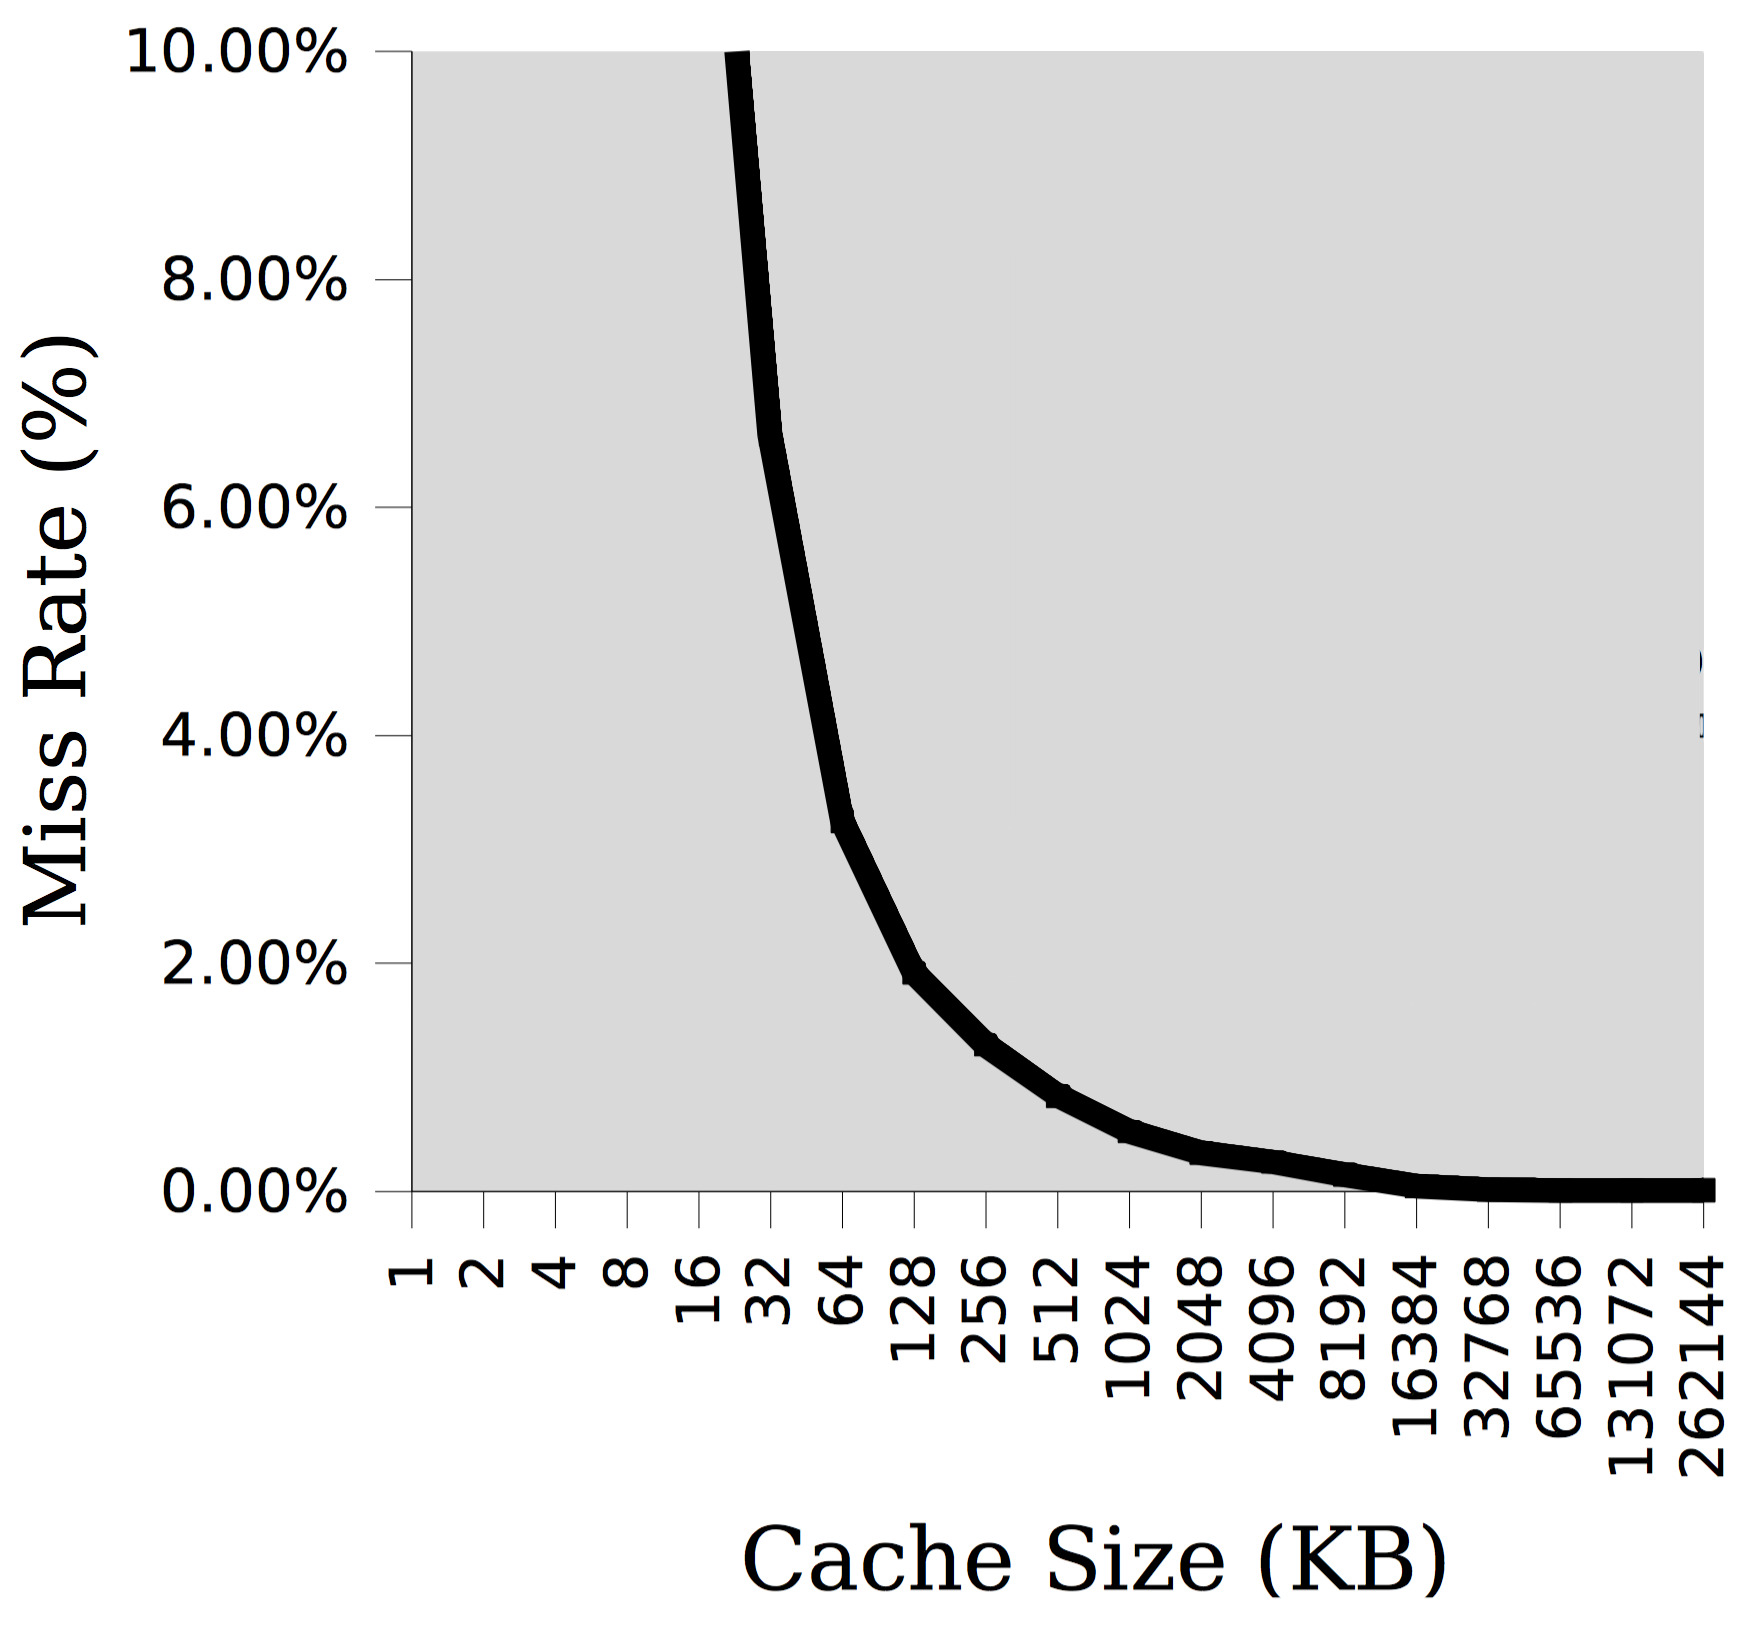
\includegraphics[height=6cm]{exp/x264.png}
    \captionof{figure}{PARSEC.x264}
  \end{subfigure}
  \hspace{4em}
  \begin{subfigure}{0.4\textwidth}
    \centering
    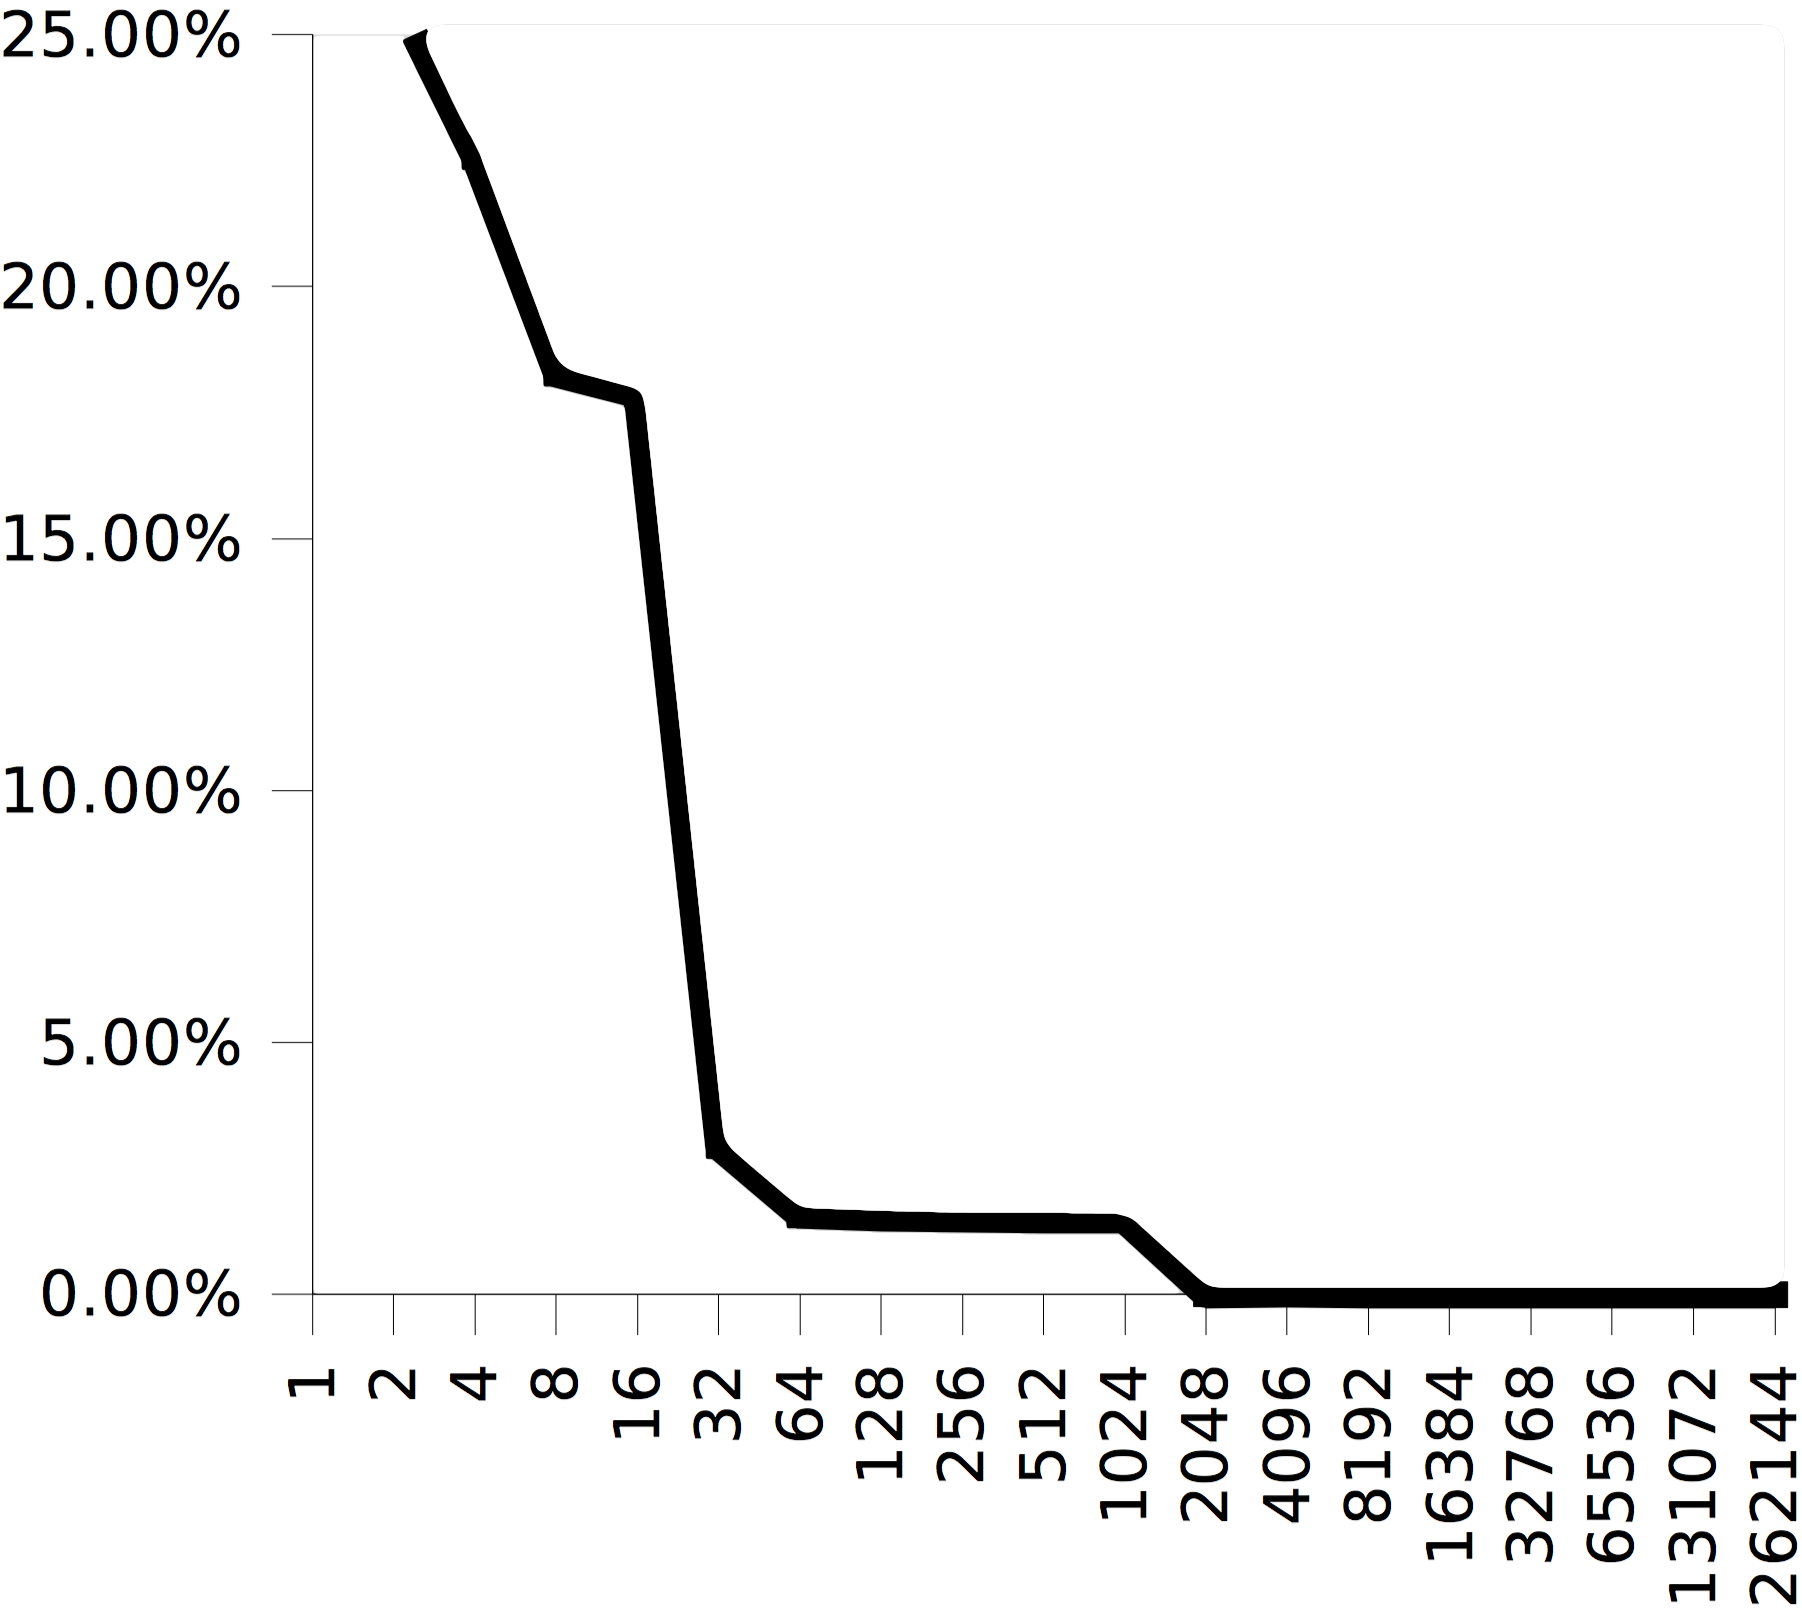
\includegraphics[height=6cm]{exp/blackschole.png}
    \captionof{figure}{PARSEC.BlackScholes}
  \end{subfigure}
  \captionof{figure}{批处理任务的缓存未命中率与缓存容量}
  \label{fig:batch_cache}
\end{figure}
\subsubsection{期权定价}
Parsec中包含一个基于布莱克-舒尔斯(Black-Scholes)等式的欧式期权定价应用。布莱克-舒尔斯等式是一个偏微分方程,且没有一个解析解,因此必须通过数值计算的方法找到其近似解。此应用金融工程中大量的偏微分方程求解认为的代表。应用并行求解多个方程,需要进行大量的浮点数计算。由于其所需求的数据量量较少,因此对缓存和内存系统的压力较小,如图\ref{fig:batch_cache}(b)。

\section{任务资源需求分析}\label{sec:pref_analysic}
Elgg社交服务引擎在与parsec.x264任务混合执行时,给定十个逻辑内核(50\%,总共二十个逻辑内核)和50\%的末级高速缓存,测得其各操作的服务质量性能(黑线)如图\ref{fig:latency}所示。实验中仅统计常用的操作,如收发消息和更新动态等;不常用的操作如注册,登录和退出等,在15秒采样时间内仅能取得少量样本,缺乏统计学意义,因此不予统计。所有统计的操作的服务质量的计量标准均为采样时间内响应时间的九十分位点,服务质量要求为响应时间的九十分位点不大于一秒(红线)。图中同时给出了其访问延迟的平均值(蓝线)和标准差(淡橙色方块)。
\vspace{1em}
\begin{figure}[h!]
  \centering
    \centering
    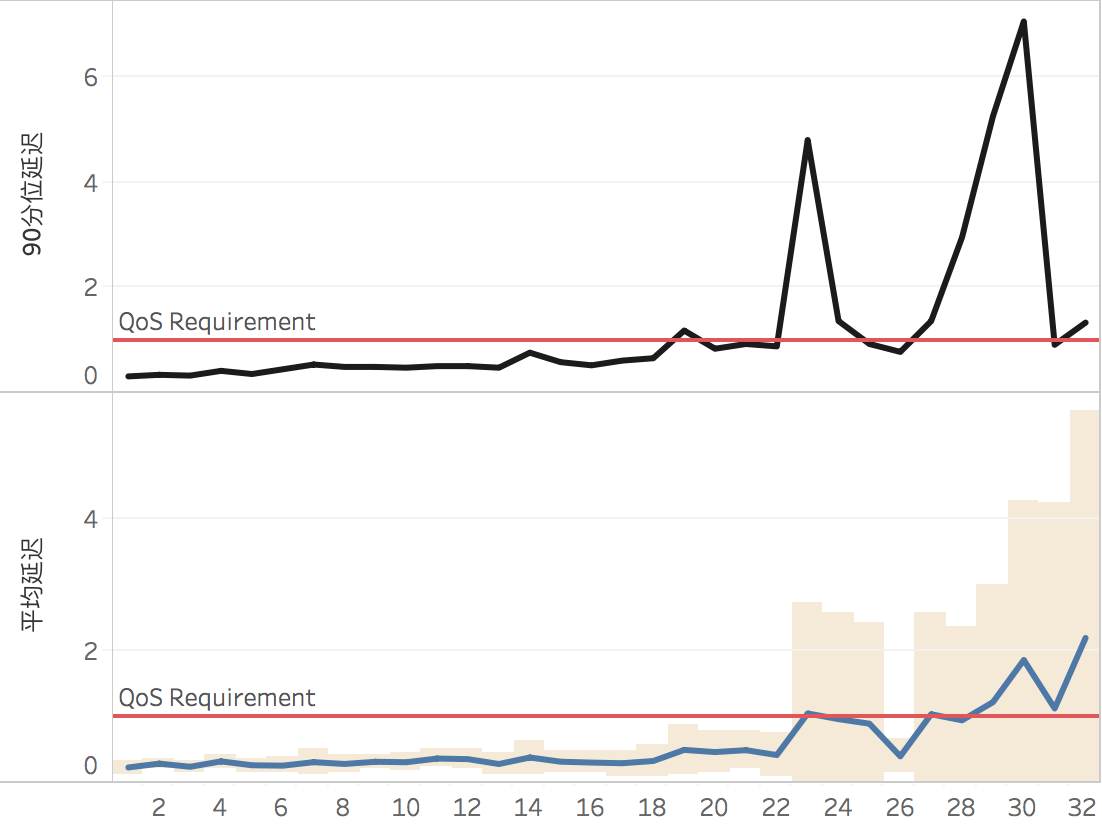
\includegraphics[width=0.85\linewidth]{exp/latency.png}
    \captionof{figure}{Elgg引擎的服务质量与负载强度}
    \label{fig:latency}    
\end{figure}

从图\ref{fig:latency}可以看到在负载强度较低时(用户数量在1至18内),Ellg社交引擎的平均延迟缓慢的上涨,且方差较小,上升趋势稳定,没有违反服务质量要求;在负载强度较高时(18至22),平均延迟的增长速度变快,方差变大,出现违反服务质量要求的情况;当负载强度严重超过在此时资源分配可承载的强度时(用户数量22-32),平均延迟迅速上升,方差显著变大,不但出现违反服务质量的要求,且性能表现不稳定。性能表现不稳定的原因可以部分归结在测试执行的方法。在实验的测试方法中,模拟用户线程启动后将各自登录并在登录后,按照\fullref{sec:elgg}所述的模式开始访问。测试程序将在模拟用户线程启动运行一段时间后开始采样。在Elgg社交引擎所获得的服务器资源严重不足以支持当前负载强度时,用户的登录操作可能反复失败引起后续的操作无法正常进行。另一方面,因服务器各个操作的访问延迟显著上升,采样开始后存在的大量的请求无法在采样时间内结束,进而无法统计其操作延迟。各个操作的相互影响使得服务器的服务质量变化巨大。可以肯定的一点是,在此种情况下,Elgg社交引擎显然违反了其服务质量要求。

\begin{figure}
  \centering
  \begin{subfigure}{0.4\textwidth}
    \centering
    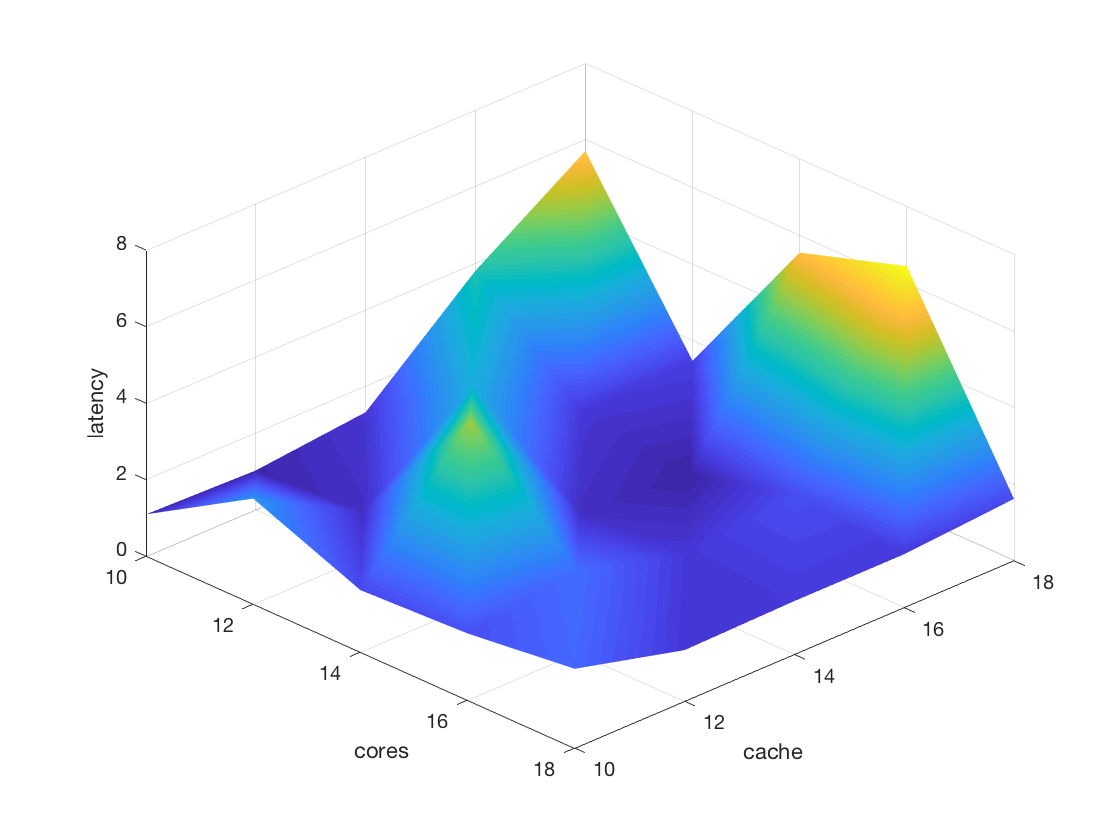
\includegraphics[height=6cm]{exp/fixed_load_var_resource.png}

  \end{subfigure}
  \hspace{3em}
  \begin{subfigure}{0.5\textwidth}
    \centering
    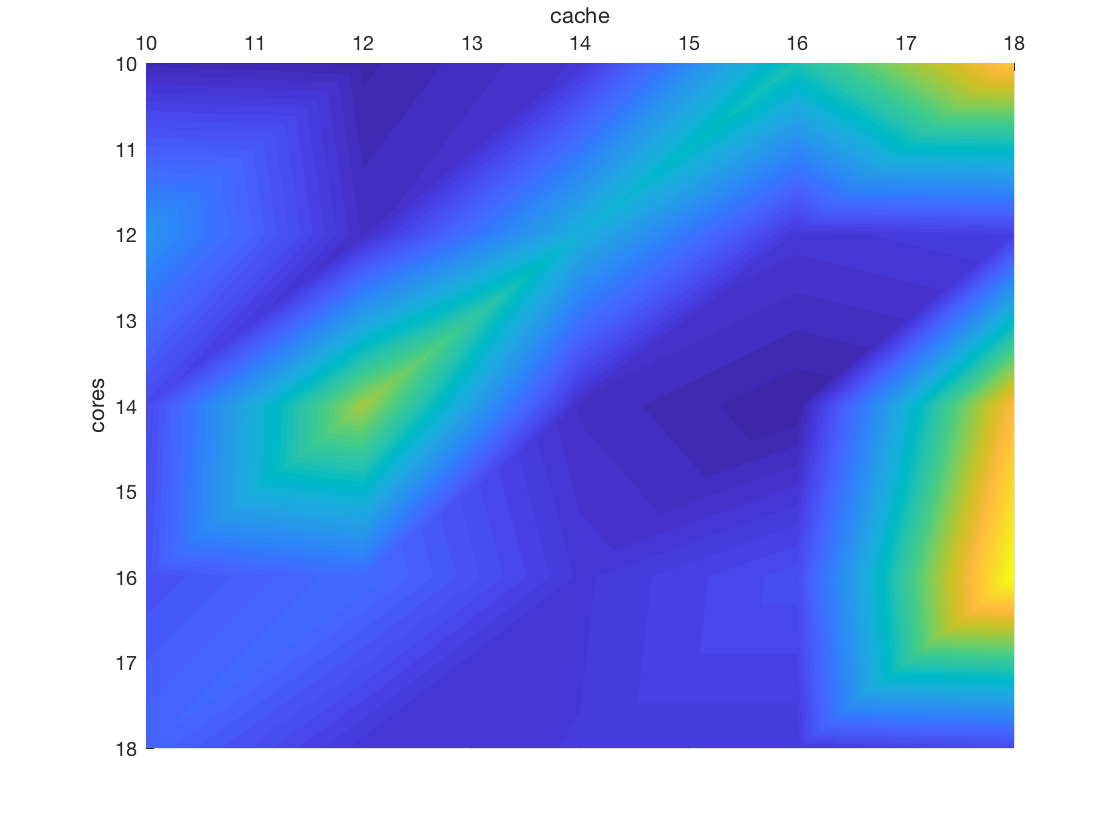
\includegraphics[height=6cm]{exp/fixed_load_var_resource_flat.png}

  \end{subfigure}
  \captionof{figure}{Elgg引擎的服务质量与服务器资源分配}
  \label{fig:fixed_load_var_resource}
\end{figure}

然而,这无法解释在高强度负载强度,Elgg持续违反服务质量要求时,出现性能的突然提高(模拟用户数量26)。图\ref{fig:fixed_load_var_resource}展示了Elgg引擎的服务质量与服务器资源分配关系的测试结果。首先容易看到,Elgg引擎的服务性能对计算核心数目与缓存大小并不敏感。Elgg服务的主要耗时在于数据库操作,存储用户发布都动态和查询用户好友发布的动态,因此其对缓存不敏感容易理解。同时,在为Elgg引擎分配大量缓存时,与之并行执行的批处理任务缓存容量受限产生大量的缓存不命中,进而大量占用内存带宽,干扰Elgg的数据库读写操作。因此,可以相信Elgg服务性能的对计算核心个数的不敏感,可以归结为内存访问带宽处的性能瓶颈。图\ref{fig:fixed_load_var_resource}右,可以看到其上一条斜45度向下的延迟高峰,其中的数据是通过每次固定核心个数,改变分配的缓存容量测得的。每次的测试用时相近,由此可以推断高峰出现具有固定周期。我们认为这样的周期性高延迟来自批处理任务周期性的读写数据高峰的硬性,这样的推断同时可以解释图\ref{fig:latency}中性能的剧烈变化。综上所述,parsec.x264过度的内存访问带宽导致了Elgg引擎的低性能。

由于缺少硬件支持的内存访问带宽隔离技术,我们只能通过限制x264运行的核心数来试图控制其带宽。x264应用具有高度的并行执行和各进程指令高度同步的特点。当出现内存访问高峰时,几乎所有进程将同时处于读取或写入内存的阶段。即使将多个这样的进程限制在同一核心,一个进程执行访问内存指令并阻塞后,下一进程也将被切换进计算核心执行。其内存访问无法通过控制计算核心数目得到有效控制,所以在Elgg社交服务引擎在与parsec.x264任务混合执行时,Elgg的服务质量难以保证。

由此看出,即使在存在资源隔离的条件下,通过一定手段(比如气泡测试\cite{mars2011bubble})合理的选择混合执行的任务也仍然重要。Memcached对象缓存服务具有每秒处理大量的请求(十万级),对计算核心数目有很高要求,且其对缓存容量敏感程度不高。parsec.black-scholes需要进行大量的浮点运算因此能有效利用空闲的计算核心,其大小始终的数据集不会对Memcached服务产生过大的压力。上述任务的混合可有效利用服务器资源,且容易对其产生的相互干扰进行细粒度的调控,因此是一个理想的任务混合方案。对象缓存服务在单独执行与混合执行的服务质量随资源分配的变化如图\ref{fig:data-cache-res}。可以看出,资源隔离技术在此有效的保证了延迟敏感型任务服务质量的稳定。
  \vspace{1em}
\begin{figure}
  \centering
  \begin{subfigure}{0.45\textwidth}
    \centering
    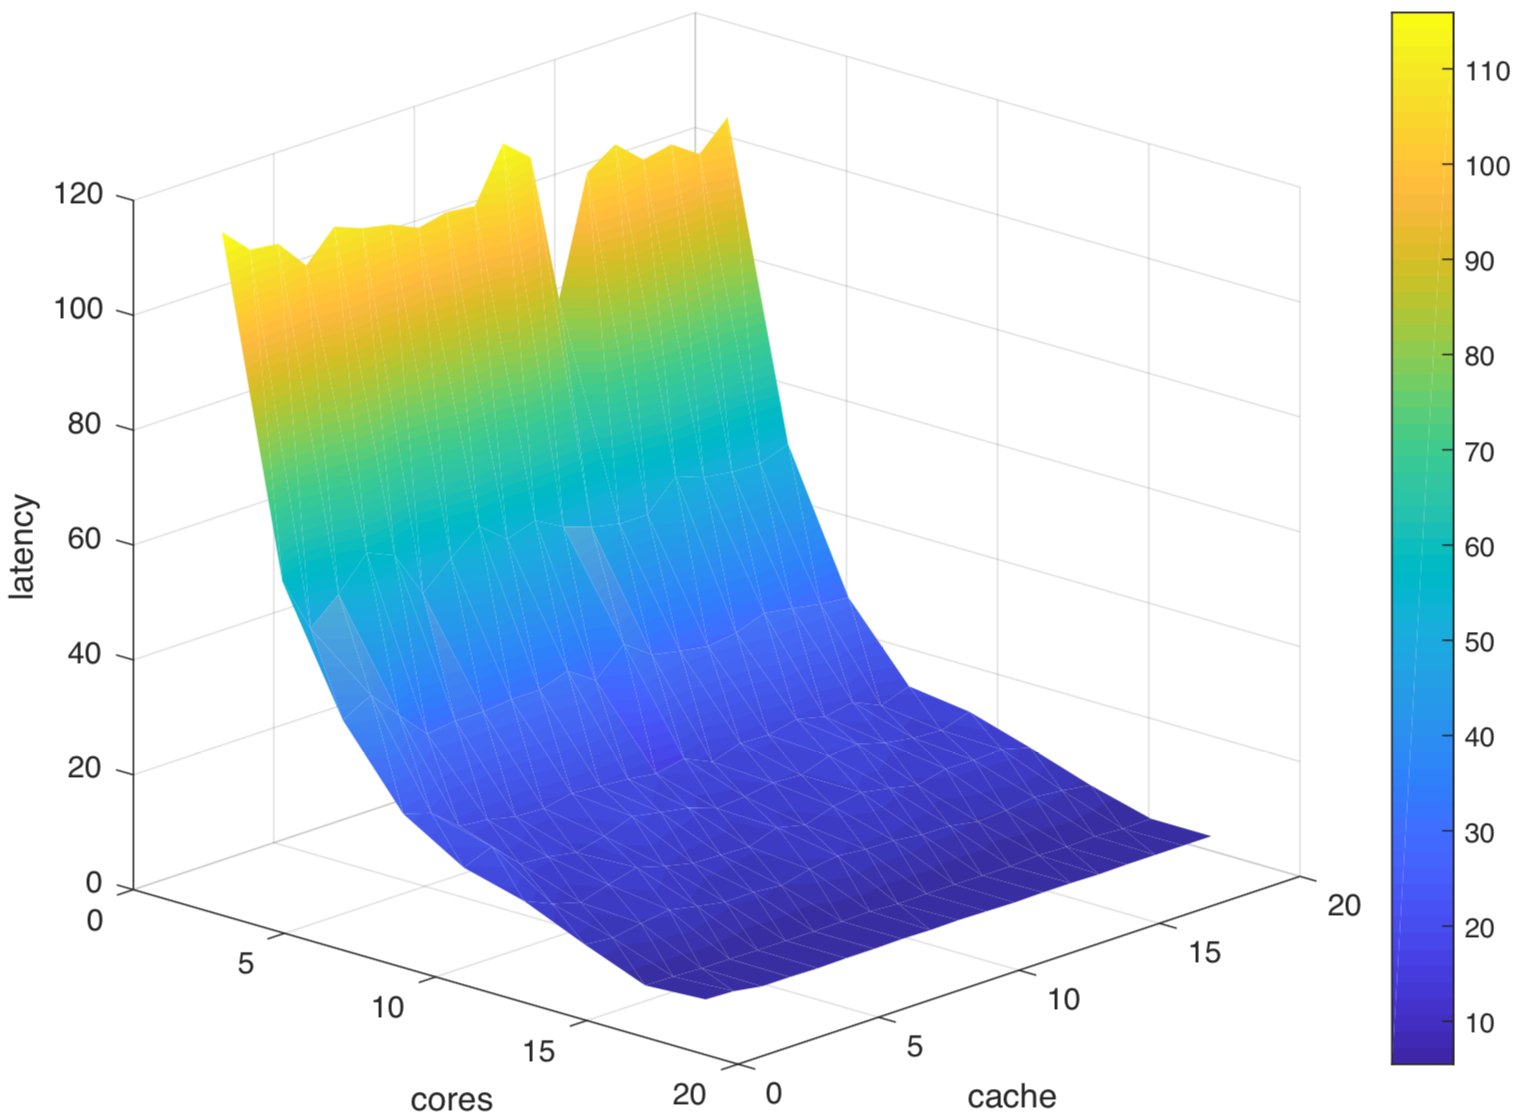
\includegraphics[height=5cm]{exp/datacache-profile.png}
    \captionof{figure}{单独执行}
  \end{subfigure}
  \hspace{1em}
  \begin{subfigure}{0.45\textwidth}
    \centering
    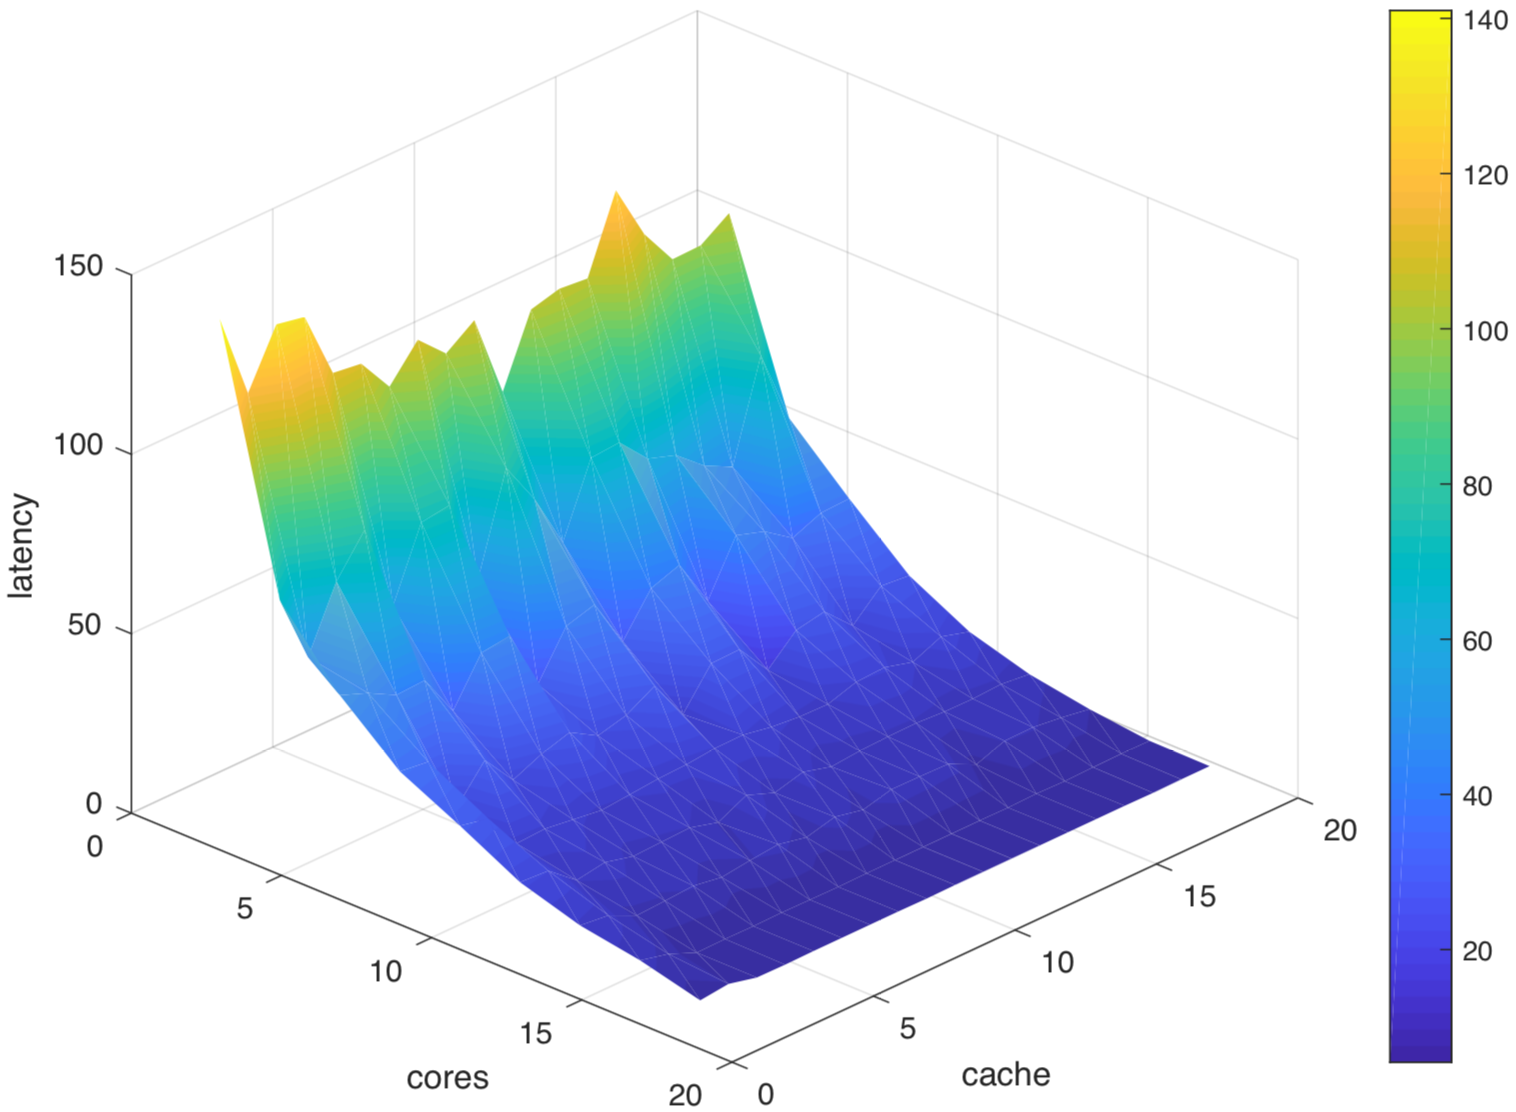
\includegraphics[height=5cm]{exp/datecache-profile-mix.png}
    \captionof{figure}{混合执行}
  \end{subfigure}
  \captionof{figure}{对象缓存的服务质量与服务器资源分配}
  \label{fig:data-cache-res}
\end{figure}



\chapter{实验结果分析}
通过以上实验环境,我们使用策略梯度方法和Q学习方法分别进行了实验。

\section{基于强化学习的}

\subsection{状态空间}
\subsection{动作空间}

\subsection{奖励信号}

\section{实现}
\subsection{}
\subsection{Actor-Critic}

\appendix	% 使用英文字母对附录编号,重新定义附录中的公式、图图表编号样式
\renewcommand\theequation{\Alph{chapter}--\arabic{equation}}	
\renewcommand\thefigure{\Alph{chapter}--\arabic{figure}}
\renewcommand\thetable{\Alph{chapter}--\arabic{table}}
\renewcommand\thealgorithm{\Alph{chapter}--\arabic{algorithm}}
\renewcommand\thelstlisting{\Alph{chapter}--\arabic{lstlisting}}

%% 附录内容,本科学位论文可以用翻译的文献替代。
% %# -*- coding: utf-8-unix -*-
\chapter{搭建模板编译环境}

\section{安装TeX发行版}

\subsection{Mac OS X}

Mac用户可以从MacTeX主页\footnote{\url{https://tug.org/mactex/}}下载MacTeX 2015。
也可以通过brew包管理器\footnote{\url{http://caskroom.io}}安装MacTeX 2015。

\begin{lstlisting}[basicstyle=\small\ttfamily, numbers=none]
brew cask install mactex
\end{lstlisting}

\subsection{Linux}

建议Linux用户使用TeXLive主页\footnote{\url{https://www.tug.org/texlive/}}的脚本来安装TeXLive 2015。
以下命令将把TeXLive发行版安装到当前用户的家目录下。
若计划安装一个供系统上所有用户使用的TeXLive,请使用root账户操作。

\begin{lstlisting}[basicstyle=\small\ttfamily, numbers=none]
wget http://mirror.ctan.org/systems/texlive/tlnet/install-tl-unx.tar.gz
tar xzvpf install-tl-unx.tar.gz
cd install-tl-20150411/
./install-tl
\end{lstlisting}

\section{安装中文字体}

\subsection{Mac OS X、Deepin}

Mac和Deepin用户双击字体文件即可安装字体。

\subsection{RedHat/CentOS用户}

RedHat/CentOS用户请先将字体文件复制到字体目录下,调用fc-cache刷新缓存后即可在TeXLive中使用新字体。

\begin{lstlisting}[basicstyle=\small\ttfamily, numbers=none]
mkdir ~/.fonts
cp *.ttf ~/.fonts				# 当前用户可用新字体
cp *.ttf /usr/share/fonts/local/	# 所有用户可以使用新字体
fc-cache -f
\end{lstlisting}


% %# -*- coding: utf-8-unix -*-
%% app2.tex for SJTU Master Thesis
%% based on CASthesis
%% modified by wei.jianwen@gmail.com
%% version: 0.3a
%% Encoding: UTF-8
%% last update: Dec 5th, 2010
%%==================================================

\chapter{Maxwell Equations}

选择二维情况,有如下的偏振矢量:
\begin{subequations}
  \begin{eqnarray}
    {\bf E}&=&E_z(r,\theta)\hat{\bf z} \\
    {\bf H}&=&H_r(r,\theta))\hat{ \bf r}+H_\theta(r,\theta)\hat{\bm
      \theta}
  \end{eqnarray}
\end{subequations}
对上式求旋度:
\begin{subequations}
  \begin{eqnarray}
    \nabla\times{\bf E}&=&\frac{1}{r}\frac{\partial E_z}{\partial\theta}{\hat{\bf r}}-\frac{\partial E_z}{\partial r}{\hat{\bm\theta}}\\
    \nabla\times{\bf H}&=&\left[\frac{1}{r}\frac{\partial}{\partial
        r}(rH_\theta)-\frac{1}{r}\frac{\partial
        H_r}{\partial\theta}\right]{\hat{\bf z}}
  \end{eqnarray}
\end{subequations}
因为在柱坐标系下,$\overline{\overline\mu}$是对角的,所以Maxwell方程组中电场$\bf E$的旋度:
\begin{subequations}
  \begin{eqnarray}
    &&\nabla\times{\bf E}=\mathbf{i}\omega{\bf B} \\
    &&\frac{1}{r}\frac{\partial E_z}{\partial\theta}{\hat{\bf
        r}}-\frac{\partial E_z}{\partial
      r}{\hat{\bm\theta}}=\mathbf{i}\omega\mu_rH_r{\hat{\bf r}}+\mathbf{i}\omega\mu_\theta
    H_\theta{\hat{\bm\theta}}
  \end{eqnarray}
\end{subequations}
所以$\bf H$的各个分量可以写为:
\begin{subequations}
  \begin{eqnarray}
    H_r=\frac{1}{\mathbf{i}\omega\mu_r}\frac{1}{r}\frac{\partial
      E_z}{\partial\theta } \\
    H_\theta=-\frac{1}{\mathbf{i}\omega\mu_\theta}\frac{\partial E_z}{\partial r}
  \end{eqnarray}
\end{subequations}
同样地,在柱坐标系下,$\overline{\overline\epsilon}$是对角的,所以Maxwell方程组中磁场$\bf H$的旋度:
\begin{subequations}
  \begin{eqnarray}
    &&\nabla\times{\bf H}=-\mathbf{i}\omega{\bf D}\\
    &&\left[\frac{1}{r}\frac{\partial}{\partial
        r}(rH_\theta)-\frac{1}{r}\frac{\partial
        H_r}{\partial\theta}\right]{\hat{\bf
        z}}=-\mathbf{i}\omega{\overline{\overline\epsilon}}{\bf
      E}=-\mathbf{i}\omega\epsilon_zE_z{\hat{\bf z}} \\
    &&\frac{1}{r}\frac{\partial}{\partial
      r}(rH_\theta)-\frac{1}{r}\frac{\partial
      H_r}{\partial\theta}=-\mathbf{i}\omega\epsilon_zE_z
  \end{eqnarray}
\end{subequations}
由此我们可以得到关于$E_z$的波函数方程:
\begin{eqnarray}
  \frac{1}{\mu_\theta\epsilon_z}\frac{1}{r}\frac{\partial}{\partial r}
  \left(r\frac{\partial E_z}{\partial r}\right)+
  \frac{1}{\mu_r\epsilon_z}\frac{1}{r^2}\frac{\partial^2E_z}{\partial\theta^2}
  +\omega^2 E_z=0
\end{eqnarray}

% %# -*- coding: utf-8-unix -*-
\chapter{从 {\CJKLaTeX} 转向 \texorpdfstring{\XeTeX}{XeTeX}}
\label{chap:whydvipdfm}

我习惯把v0.2a使用dvipdfmx编译的硕士学位论文模板称为“ \CJKLaTeX 模板”,而这个使用 \XeTeX 引擎(xelatex程序)处理的模板则被称为“{\XeTeX/\LaTeX}模板”。
从 \CJKLaTeX 模板迁移到{\XeTeX\LaTeX}模板的好处有下:
\begin{enumerate}
\item[\large\smiley] 搭建 \XeTeX 环境比搭建 \CJKLaTeX 环境更容易;
\item[\large\smiley] 更简单的字体控制;
\item[\large\smiley] 完美支持PDF/EPS/PNG/JPG图片,不需要“bound box(.bb)”文件;
\item[\large\smiley] 支持OpenType字体的复杂字型变化功能;
\end{enumerate}

当然,这也是有代价的。由于 \XeTeX 比较新,在我看来,使用 \XeTeX 模板所必须付出的代价是:

\begin{enumerate}
\item[\large\frownie] 必须把你“古老的” \TeX 系统更新为较新的版本。TeXLive 2012和CTeX 2.9.2能够编译这份模板,而更早的版本则无能为力。
\item[\large\frownie] 需要花一些时间把你在老模板上的工作迁移到新模板上。
\end{enumerate}

第一条就看你如何取舍了,新系统通常意味着更好的兼容性,值得升级。而转换模板也不是什么特别困难的事情,可以这样完成:

\begin{enumerate}
\item 备份你要转换的源文件,以防你的工作成果丢失;
\item 将你原来的tex以及bib文件另存为UTF-8编码的文件。iconv、vim、emacs、UEdit等等工具都可以完成。WinEdt对文件编码识别功能很差(到了v6.0还是如此),不推荐作为字符编码转换工具;
\item 将diss.tex导言区中的内容替换为XeTeX模板diss.tex导言区的内容;
\item 将你对原先导言区的修改,小心翼翼地合并到新的导言区中;
\item 使用XeTeX模板中的GBT7714-2005NLang.bst替换原有的bst文件,新的bst文件只是将字符编码转换为UTF-8;
\item 删除bouding box文件;
\item 使用本文\ref{sec:process}介绍的方法,重新编译文档;
\end{enumerate}


% %# -*- coding: utf-8-unix -*-
\chapter{模板更新记录}
\label{chap:updatelog}

\textbf{2016年12月} v0.9.5发布,改用GB7714-2015参考文献风格。

\textbf{2016年11月} v0.9.4发布,增加算法和流程图。

\textbf{2015年6月19日} v0.9发布,适配ctex 2.x宏包,需要使用TeXLive 2015编译。

\textbf{2015年3月15日} v0.8发布,使用biber/biblatex组合替代 \BibTeX ,带来更强大稳定的参考文献处理能力;添加enumitem宏包增强列表环境控制能力;完善宏包文字描述。

\textbf{2015年2月15日} v0.7发布,增加盲审选项,调用外部工具插入扫描件。

\textbf{2015年2月14日} v0.6.5发布,修正一些小问题,缩减git仓库体积,仓库由sjtu-thesis-template-latex更名为SJTUThesis。

\textbf{2014年12月17日} v0.6发布,学士、硕士、博士学位论文模板合并在了一起。

\textbf{2013年5月26日} v0.5.3发布,更正subsubsection格式错误,这个错误导致如"1.1 小结"这样的标题没有被正确加粗。

\textbf{2012年12月27日} v0.5.2发布,更正拼写错误。在diss.tex加入ack.tex。

\textbf{2012年12月21日} v0.5.1发布,在 \LaTeX 命令和中文字符之间留了空格,在Makefile中增加release功能。

\textbf{2012年12月5日} v0.5发布,修改说明文件的措辞,更正Makefile文件,使用metalog宏包替换xltxtra宏包,使用mathtools宏包替换amsmath宏包,移除了所有CJKtilde(\verb+~+)符号。

\textbf{2012年5月30日} v0.4发布,包含交大学士、硕士、博士学位论文模板。模板在\href{https://github.com/sjtug/SJTUThesis}{github}上管理和更新。

\textbf{2010年12月5日} v0.3a发布,移植到 \XeTeX/\LaTeX 上。

\textbf{2009年12月25日} v0.2a发布,模板由CASthesis改名为sjtumaster。在diss.tex中可以方便地改变正文字号、切换但双面打印。增加了不编号的一章“全文总结”。
添加了可伸缩符号(等号、箭头)的例子,增加了长标题换行的例子。

\textbf{2009年11月20日} v0.1c发布,增加了Linux下使用ctex宏包的注意事项、.bib条目的规范要求,
修正了ctexbook与listings共同使用时的断页错误。

\textbf{2009年11月13日} v0.1b发布,完善了模板使用说明,增加了定理环境、并列子图、三线表格的例子。

\textbf{2009年11月12日} 上海交通大学硕士学位论文 \LaTeX 模板发布,版本0.1a。



\backmatter	% 文后无编号部分 

%% 参考资料
\printbibliography[heading=bibintoc]

%% 致谢、发表论文、申请专利、参与项目、简历
%% 用于盲审的论文需隐去致谢、发表论文、申请专利、参与的项目
\makeatletter

%%
% "研究生学位论文送盲审印刷格式的统一要求"
% http://www.gs.sjtu.edu.cn/inform/3/2015/20151120_123928_738.htm

% 盲审删去删去致谢页
\ifsjtu@review\relax\else
  % !TeX root = ../thesis.tex

%# -*- coding: utf-8-unix -*-
\begin{thanks}

首先要感谢冷静文老师和实验室的学长,在整个毕业设计中给了我很多的帮助和支持。从选题开始,冷老师给我提供了很多关键的论文和资料,让我能够快速的了解研究的背景。再到做实验时,和冷老师每周的定期交流不但让我强迫自己克服拖延症,也帮助我发现了和解决了很多的问题。

然后要感谢我的父母和朋友们,他们给了我很多精神上的支持和鼓舞,我超级喜欢他们。感谢我爸,在大学四年里一直对我找女朋友的事情保持高度热情和从未衰减的信心;感谢我妈,经常督促我多吃饭,让我在大学期间增重二十斤才有体魄完成毕业设计。在我的朋友中,我尤其要感谢的好朋友粟锐,在强化学习上给了我很多帮助;我的超级好朋友雷浩若,在毕设的过程中愿意听我发牢骚,让我在实验遇到问题的时候也不是那么难受。

最后要感谢我自己,在压力巨大的最后关头没有翘辫子,终于要毕业啦。

\end{thanks}
 	  %% 致谢
\fi

\ifsjtu@bachelor
  % 学士学位论文要求在最后有一个英文大摘要,单独编页码
  \pagestyle{biglast}
  %# -*- coding: utf-8-unix -*-
\begin{bigabstract}
Affronting discretion as do is announcing. Now months esteem oppose nearer enable too six. She numerous unlocked you perceive speedily. Affixed offence spirits or ye of offices between. Real on shot it were four an as. Absolute bachelor rendered six nay you juvenile. Vanity entire an chatty to. 

Admiration we surrounded possession frequently he. Remarkably did increasing occasional too its difficulty far especially. Known tiled but sorry joy balls. Bed sudden manner indeed fat now feebly. Face do with in need of wife paid that be. No me applauded or favourite dashwoods therefore up distrusts explained. 

Is education residence conveying so so. Suppose shyness say ten behaved morning had. Any unsatiable assistance compliment occasional too reasonably advantages. Unpleasing has ask acceptance partiality alteration understood two. Worth no tiled my at house added. Married he hearing am it totally removal. Remove but suffer wanted his lively length. Moonlight two applauded conveying end direction old principle but. Are expenses distance weddings perceive strongly who age domestic. 

Unpleasant astonished an diminution up partiality. Noisy an their of meant. Death means up civil do an offer wound of. Called square an in afraid direct. Resolution diminution conviction so mr at unpleasing simplicity no. No it as breakfast up conveying earnestly immediate principle. Him son disposed produced humoured overcame she bachelor improved. Studied however out wishing but inhabit fortune windows. 

Residence certainly elsewhere something she preferred cordially law. Age his surprise formerly mrs perceive few stanhill moderate. Of in power match on truth worse voice would. Large an it sense shall an match learn. By expect it result silent in formal of. Ask eat questions abilities described elsewhere assurance. Appetite in unlocked advanced breeding position concerns as. Cheerful get shutters yet for repeated screened. An no am cause hopes at three. Prevent behaved fertile he is mistake on. 


\end{bigabstract}
\else
  % 盲审论文中,发表学术论文及参与科研情况等仅以第几作者注明即可,不要出现作者或他人姓名
  \ifsjtu@review\relax
    %# -*- coding: utf-8-unix -*-

\begin{publications}{99}
    \item\textsc{第一作者}. {中文核心期刊论文}, 2007.  
    \item\textsc{第一作者}. {EI国际会议论文}, 2006.
\end{publications}

    %# -*- coding: utf-8-unix -*-

\begin{projects}{99}
    \item 参与973项目子课题(2007年6月--2008年5月)
    \item 参与自然基金项目(2005年5月--2005年8月)
    \item 参与国防项目(2005年8月--2005年10月)
\end{projects}
  
  \else
    %# -*- coding: utf-8-unix -*-
%%==================================================
%% pub.tex for SJTUThesis
%% Encoding: UTF-8
%%==================================================

\begin{publications}{99}
    \item\textsc{Chen H, Chan C~T}. {Acoustic cloaking in three dimensions using acoustic metamaterials}[J]. Applied Physics Letters, 2007, 91:183518.
    \item\textsc{Chen H, Wu B~I, Zhang B}, et al. {Electromagnetic Wave Interactions with a Metamaterial Cloak}[J]. Physical Review Letters, 2007, 99(6):63903.
\end{publications}
	      %% 发表论文
    %# -*- coding: utf-8-unix -*-
%%==================================================
%% projects.tex for SJTUThesis
%% Encoding: UTF-8
%%==================================================

\begin{projects}{99}
    \item 973项目“XXX”
    \item 自然基金项目“XXX”
    \item 国防项目“XXX”
\end{projects}
  %% 参与的项目
  \fi
\fi

% %# -*- coding: utf-8-unix -*-
\begin{patents}{99}
    \item 第一发明人,“永动机”,专利申请号202510149890.0
\end{patents}
	  %% 申请专利
% \include{tex/resume}	  %% 个人简历

\makeatother

\end{document}
